
\begin{itemize} 
\item mention that only 8 TeV selection will be discussed here. 7 TeV selections 
      can be referred to [7TeV paper?].
\item should mention that which channel is more sensitive and which method is used 
      in which final states 
\end{itemize} 



The analysis strategy is the following. We first select events with 
a pair of oppositely-charged leptons, electrons($e^\pm$) or muons($\mu^\pm$) 
with \pt\ requirement that maximum(minimum) of the lepton \pt\ should be 
greater than 20(10)~\GeV. This choice of \pt\ cut is due to trigger requirement. 
Then, we apply a baseline selection for basic objects such as leptons, jets, \met, .... 
as well as for specific background processes. This baseline selection is called 
``WW selection" because after applying it we end up with choosing two W's.   

The background composition depends on the number of jets and the lepton flavors. 
For example, in the 0-jet \DF\ channel, the non-resonant WW is the main 
background and in the 1-jet \DF\ channel, \topbkg is the leading background process. 
The full spectrum of the background composition is discussed in chapter~\ref{ch:background_estimation}. 
Therefore, the analsys is optimized in different channels depending on  
the number of jets and the lepton flavors. This analysis is dedicated 
to search for \ggH\ process, events with 2 or more jets are not considered 
because this region of phase space is used to study \qqH\ process. 
We thus have two categories in number of jets(0-jet or 1-jet) 
and two categories in lepton flavors(\DF or \SF). 
Therefore, we have four channels.

Extraction of signal component is done by two methods. First method which is simpler
but less sensitive to discovery is ``cut-based" method. This method is a simple cut-and-count approach 
which maximizes the signal to background ratio(S/B) at a given Higgs mass. Accounting for the 
kinematic difference between different \mHi\ which was discussed in 
section~\ref{subsec:kinimetic_variables}, the selections are optimized for a 
given higgs mass. This method is applied to all lepton flavor final states. 
The other method which is more complicated and sophiscated but more sensitive to discovery 
is ``2D" method which uses binned 2-dimensional templates of \mT\ and \mll. 
Binned maximum likelihood fit to the 2D templates is done to extract 
the signal component. Most of the templates are taken from simulation 
so it is important to ensure that the shapes in simulation are consistent 
with data. In \SF\ channel \dyll\ is one of the leading backgrounds. 
The shape of \dyll\ taken from simulation is not reliable because of 
poor modeling of \met\ and poot statistics in the sample. So, we apply 
this method to only \DF\ channel. 



\section{Baseline selection : WW selection} 
\begin{itemize} 
\item additional selections : Third lepton veto, $\mll>12~\GeV$, $\ptll>30(45)~\GeV$ 
\item Z veto and DY MVA for SF  
%DY MVA : https://indico.cern.ch/getFile.py/access?contribId=45&sessionId=0&resId=0&materialId=slides&confId=208848
\item Make a cut summary table like below that summarizes WW selection. 
      % https://twiki.cern.ch/twiki/bin/view/CMSPublic/Hig13003TWiki
      \begin{figure}[htp] 
      \centering 
      \begin{tabular}{c} 
%      \includegraphics[height=10cm]{figures/temp_ww_sel.png} 
      \end{tabular} 
      \end{figure}   
\end{itemize} 



\subsubsection{Additional selections} 
In addition to the requirements discussed in chapter~\ref{ch:event_reconstruction_selection},   
we apply additional cuts to suppress specific source of backgrounds.  
Events which have third lepton with $\pt>10~\GeV$ are rejected to suppress contributions 
from \vv.
In order to reject low mass di-lepton resonances, $\mll>12~\GeV$ is applied. 
The \dyll\ background is suppressed by Z mass veto which requires that 
$\left| M_Z - \mll \right| > 15~\GeV$.
\Wjets\ background tends to have small \ptll\ because the lepton from W and 
the recoiling jet are likely to be back-to-back. So, in order to suppress 
\Wjets\ more, $\ptll>30(45)~\GeV$ is applied for shape-based (cut-based) apporoaches. 

\subsubsection{MVA(BDT)-based \dyll\ suppression} 

In the \SF\ channels, \dyll\ is one of the dominant backgrouds 
and one typically impose tight \met\ cut to suppress this background. 
But, as shown in~\ref{fig:projmet}, tightening \met\ selection
can lead to significant loss in signal. So, we developed an 
MVA(BDT)-based \dyll\ suppression technique. 

The training is done with a combination of signal samples, \mHi = 125 and 200~\GeV, 
for signal and \dyll\ MC for background. Motivation of using a combination of two 
\mHi\ points is to use one training across all \mHi points. For background, a 
combination of Madgraph and Powheg samples is used to maximize statistics. 
In order for the training to be consistent with the analysis where it is actually 
applied, the same selection is applied such that we use the same phase space 
for training as the application. All baseline selections for cut-based analysis 
in the \SF\ final states mentioned in chapter~\ref{ch:event_reconstruction_selection} 
and this section are applied except for \mT\ cut because it is an effectively cut on \met
and $\ptll>30\GeV$ because .... 
The training is done separately in the 0-jet and 1-jet catagories. 

The input variables for the training are the following. 
\begin{itemize}

%
\item \met-related variables
\begin{itemize}
\item \pmet 
\item \ptrkmet  
\item \met\ significance : 
      $\displaystyle \frac{\met}{\sqrt{\sum_{i}^{\textrm{All objects}} E_T(i)}}$
      where $E_T(i)$ is the tranverse energy of object i that was used for \met\ calculation
\end{itemize}

%
\item kinematic variables
\begin{itemize}
\item \ptll : di-lepton \pt 
\item \mT : Higgs transverse mass 
\item leading jet \pt
\item recoil of di-lepton + \met\ system   
\end{itemize}

%
\item azimuthal angle differences 
\begin{itemize}
\item $\Delta\phi(ll, \textrm{leading jet})$ : azimuthal angle difference between di-lepton system 
      and the leading jet ($\pt>15~\GeV$)
\item $\Delta\phi(ll, \met)$ : azimuthal angle difference between di-lepton system 
      and \met
\item $\Delta\phi(\textrm{leading jet}, \met)$ : azimuthal angle difference between 
      the leading jet ($\pt>15~\GeV$) and \met
\end{itemize}

%
\item other variable
\begin{itemize}
\item $N_{vtx}$ : number of reconstructed vertices 
\end{itemize}

\end{itemize}

\begin{figure}[htp] 
\centering
\begin{tabular}{c} 
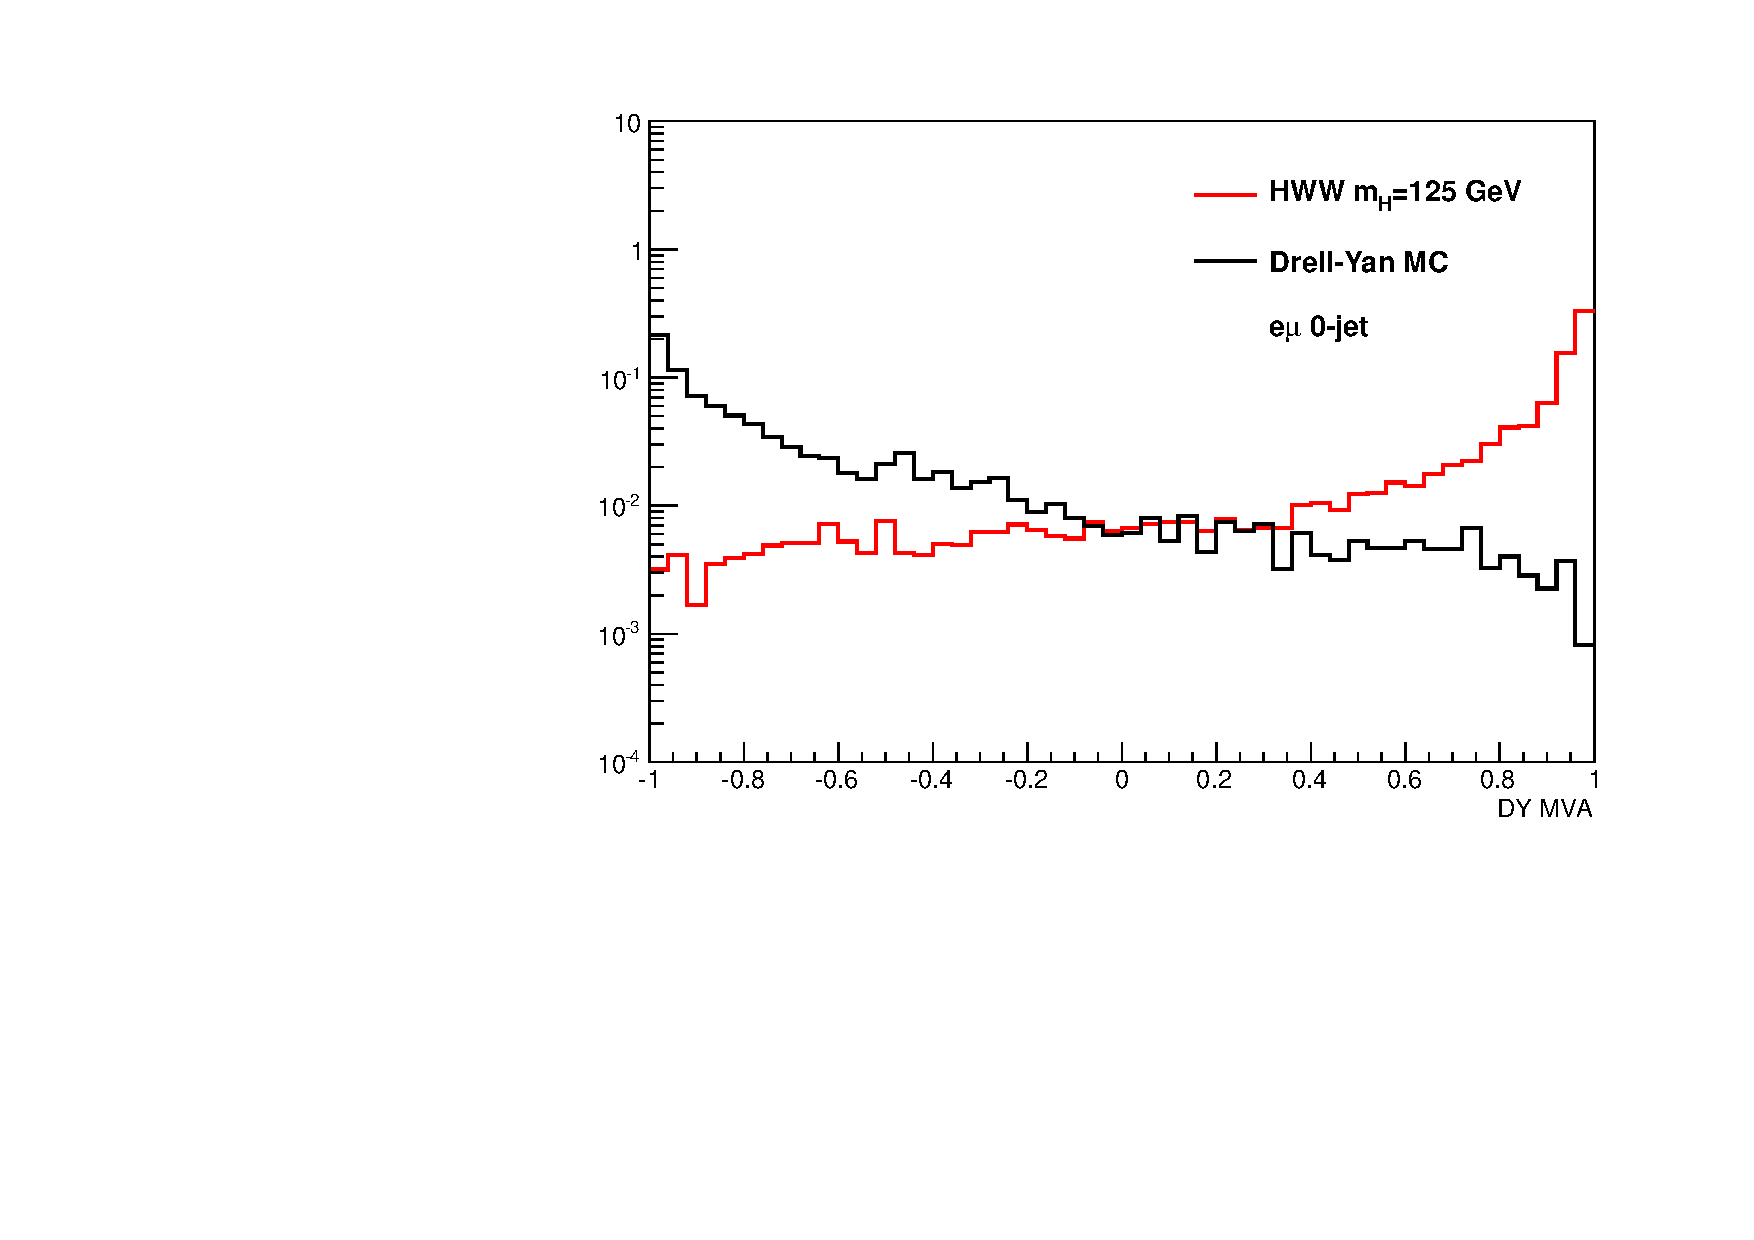
\includegraphics[width=0.5\textwidth]{figures/dymva_0j.pdf} 
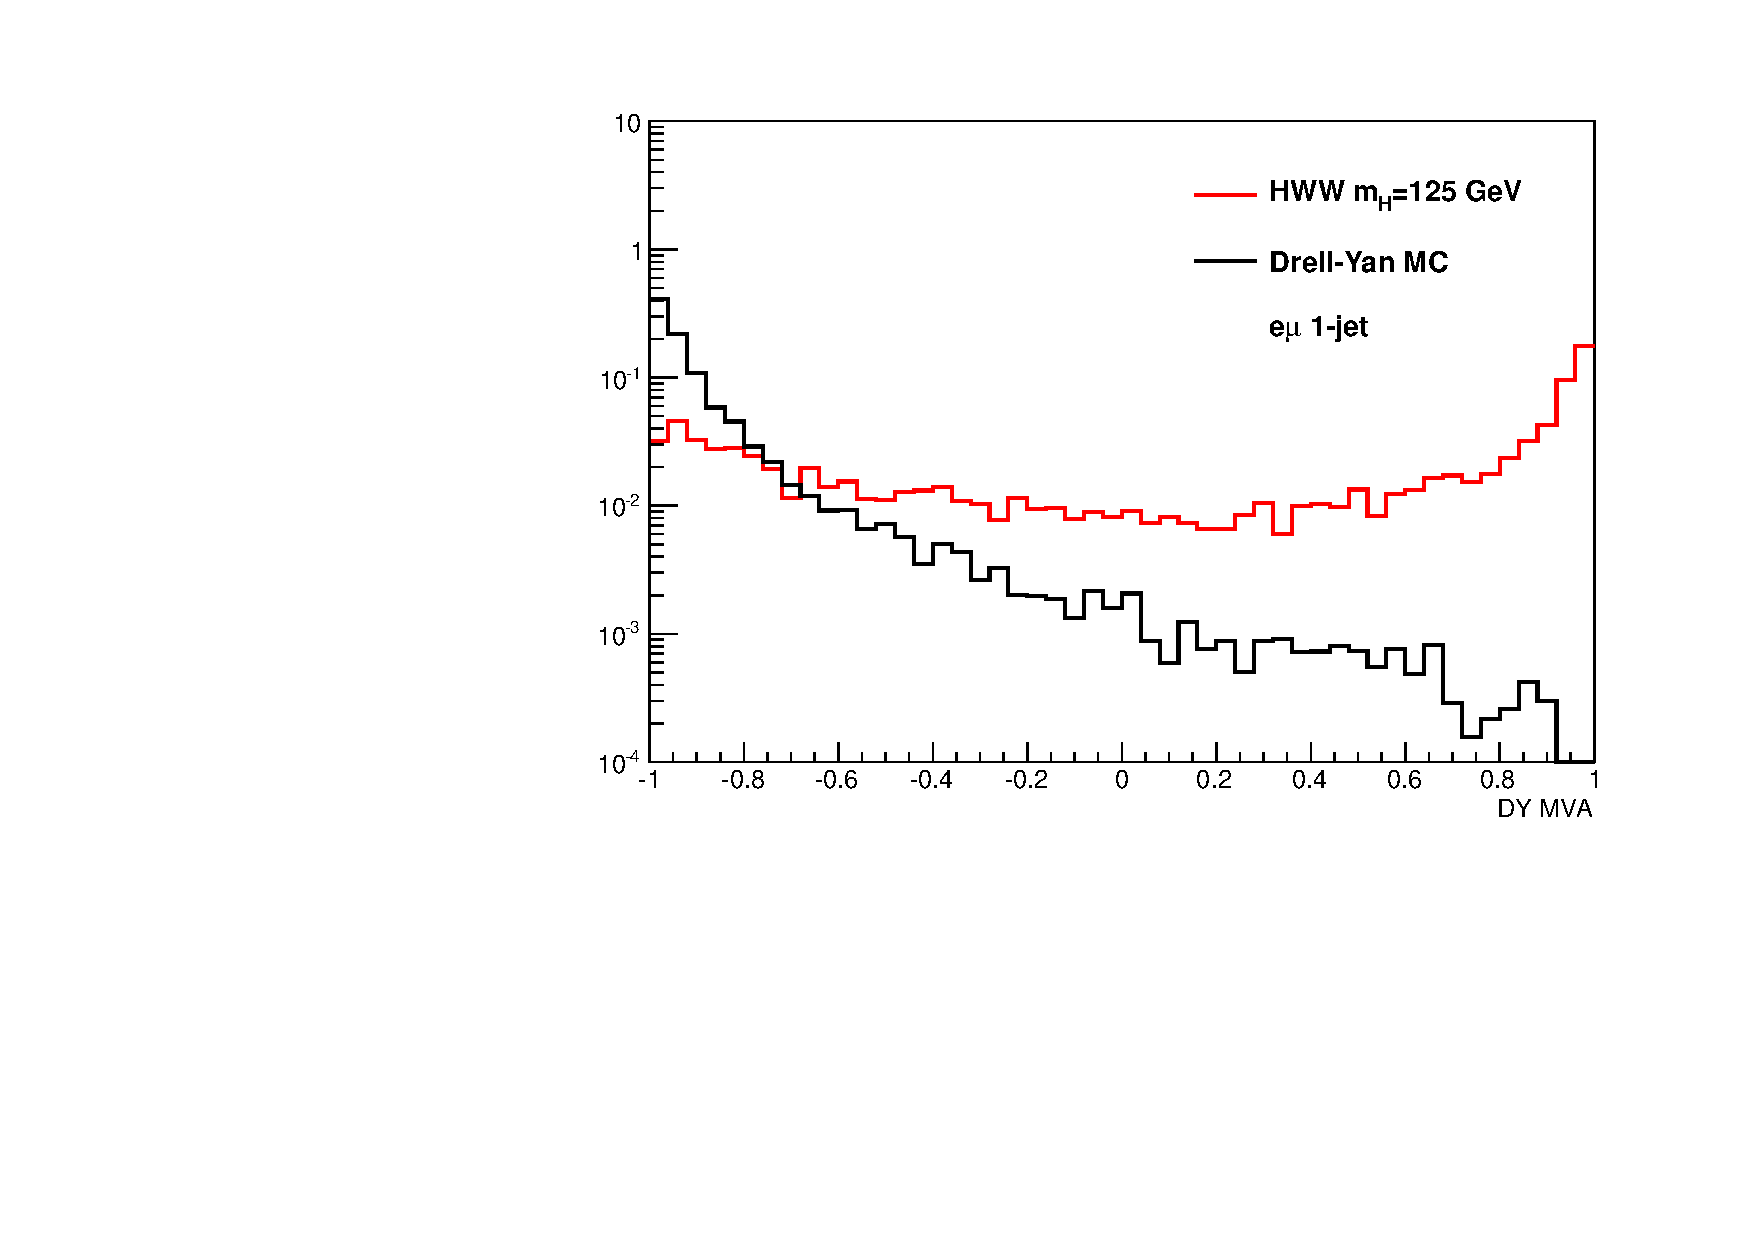
\includegraphics[width=0.5\textwidth]{figures/dymva_1j.pdf} 
\end{tabular} 
\caption{The BDT output(BDT) for \mHi = 125~\GeV(red) and \dyll\ MC(black)
in 0-jet(left) and 1-jet(right) categories.} 
\label{fig:dymva} 
\end{figure} 

Figure~\ref{fig:dymva} shows the output of BDT(DY MVA) for \mHi = 125~\GeV in red 
and \dyll\ MC in black in 0-jet(left) and 1-jet(right) categories. We finally require 
that DY MVA be greater than 0.88(0.84) in 0-jet(1-jet) category. This requirement 
is applied to only \SF\ category, the \DF\ category has only $\minpmet>20~\GeV$.

All requirements imposed so far area basically to select events with 
a pair of W. This baseline selection is called ``WW selection" and 
the state of events where WW selection is applied is called ``WW level".
By applying WW selection, we can reach better signal-to-background ratio(S/B)
and reasonable extraction of signal can be possible. 
Table~\ref{tab:wwselection} shows a summary of requirements for WW selection. 

\begin{table}[htp] 
\begin{center} 
\begin{tabular}{c|cc}
\hline
Selection & \DF & \SF \\
\hline \hline 
\ptlmax & $>20~\GeV$ & $>20~\GeV$ \\
\ptlmin & $>10~\GeV$ & $>10~\GeV$ \\
Lepton selection & applied & applied \\
Number of jet selection & applied & applied \\
Third lepton veto & applied & applied \\
opposite-sign requirement & applied & applied \\
\mll & $>12~\GeV$ & $>12~\GeV$ \\
$\left| \mll - m_Z \right| > 15~\GeV$ & not applied & applied \\
\minpmet & $>20~\GeV$ & $>20~\GeV$ \\
MVA-based Drell-Yan suppression & not applied & applied \\
Top veto & applied & applied \\
\ptll & $>30~\GeV$[*] & $>45~\GeV$ \\
\hline
\end{tabular} 
\caption{Summary of WW selection. [*] For shape-based method 
$\ptll>30~\GeV$ is applied and for cut-based method $\ptll>45~\GeV$ is applied.}
\label{tab:wwselection} 
\end{center} 
\end{table} 

%%%%%%%%%%%%%%%%%%%%%%%%%%%%%%%%%%%%%%%
\section{Cut-based Method}

%\begin{itemize} 
%\item Motivation of \mHi-dependent cuts : event kinematics different by \mHi 
%\item Physics behind cuts : (1) helicity conservation and V-A nature of W decay (2) more massive Higgs gives harder leptons  
%\item list cut variables: \ptlmax, \ptlmin, \mll, \delphill, \mT 
%\item justify \mHi-dependent cut values : make plots of signal at \mHi=125, 160, 200, 400 GeV
%\item Show the table of \mHi-dependent cuts : make sure that numbers are up-to-date  
%\end{itemize} 

The first method used to extract signal component is the "cut-based" method. 
It is a cut-and-count method and a robust baseline method for this analysis. 
In this approach, at each \mHi\ expected signal and background yields are 
calculated in the region of the phase space where S/B is maximized. 
The yields and uncertainties are used to determine the signal component 
by maximum likelihood fit. Given that there is no phase space that can 
constrain the estimated uncertainty, the uncertainty estimation is very important.  
This method is simpler than the other method becasue it uses only yields 
and most of the backgrounds are extimated by data-driven methods. 
The issue is the accuracy of the estimation and the uncertainty.  

As described in section~\ref{subsec:kinimetic_variables}, the kinematics of 
the signal events vary depending on \mHi. Therefore, 
in addition to the WW selection, dedicated selection 
for a \mHi\ point is applied to maximize the sensitivity at the given mass. 
We use the following five variables to improve S/B, 
\begin{itemize}
\item lepton transeverse momentum : \ptlmax, \ptlmin
\item di-lepton mass : \mll 
\item the azimuthal angle difference between leptons : \delphill
\item Higgs transverse mass : 
\begin{eqnarray} 
\mT = \sqrt{2\ptll\met(1-cos(\Delta\phi_{\ell\ell-\met}))}
\end{eqnarray} 
where \ptll\ is transverse momentum of the dilepton system,
\met\ is missing transverse momentum, and
$\Delta\phi_{\ell\ell-\met}$ is the angle between dilepton
direction and \met\ in the transverse plane.
\end{itemize}

% WW-level mH = 125 GeV
\begin{figure}[htp]
\centering
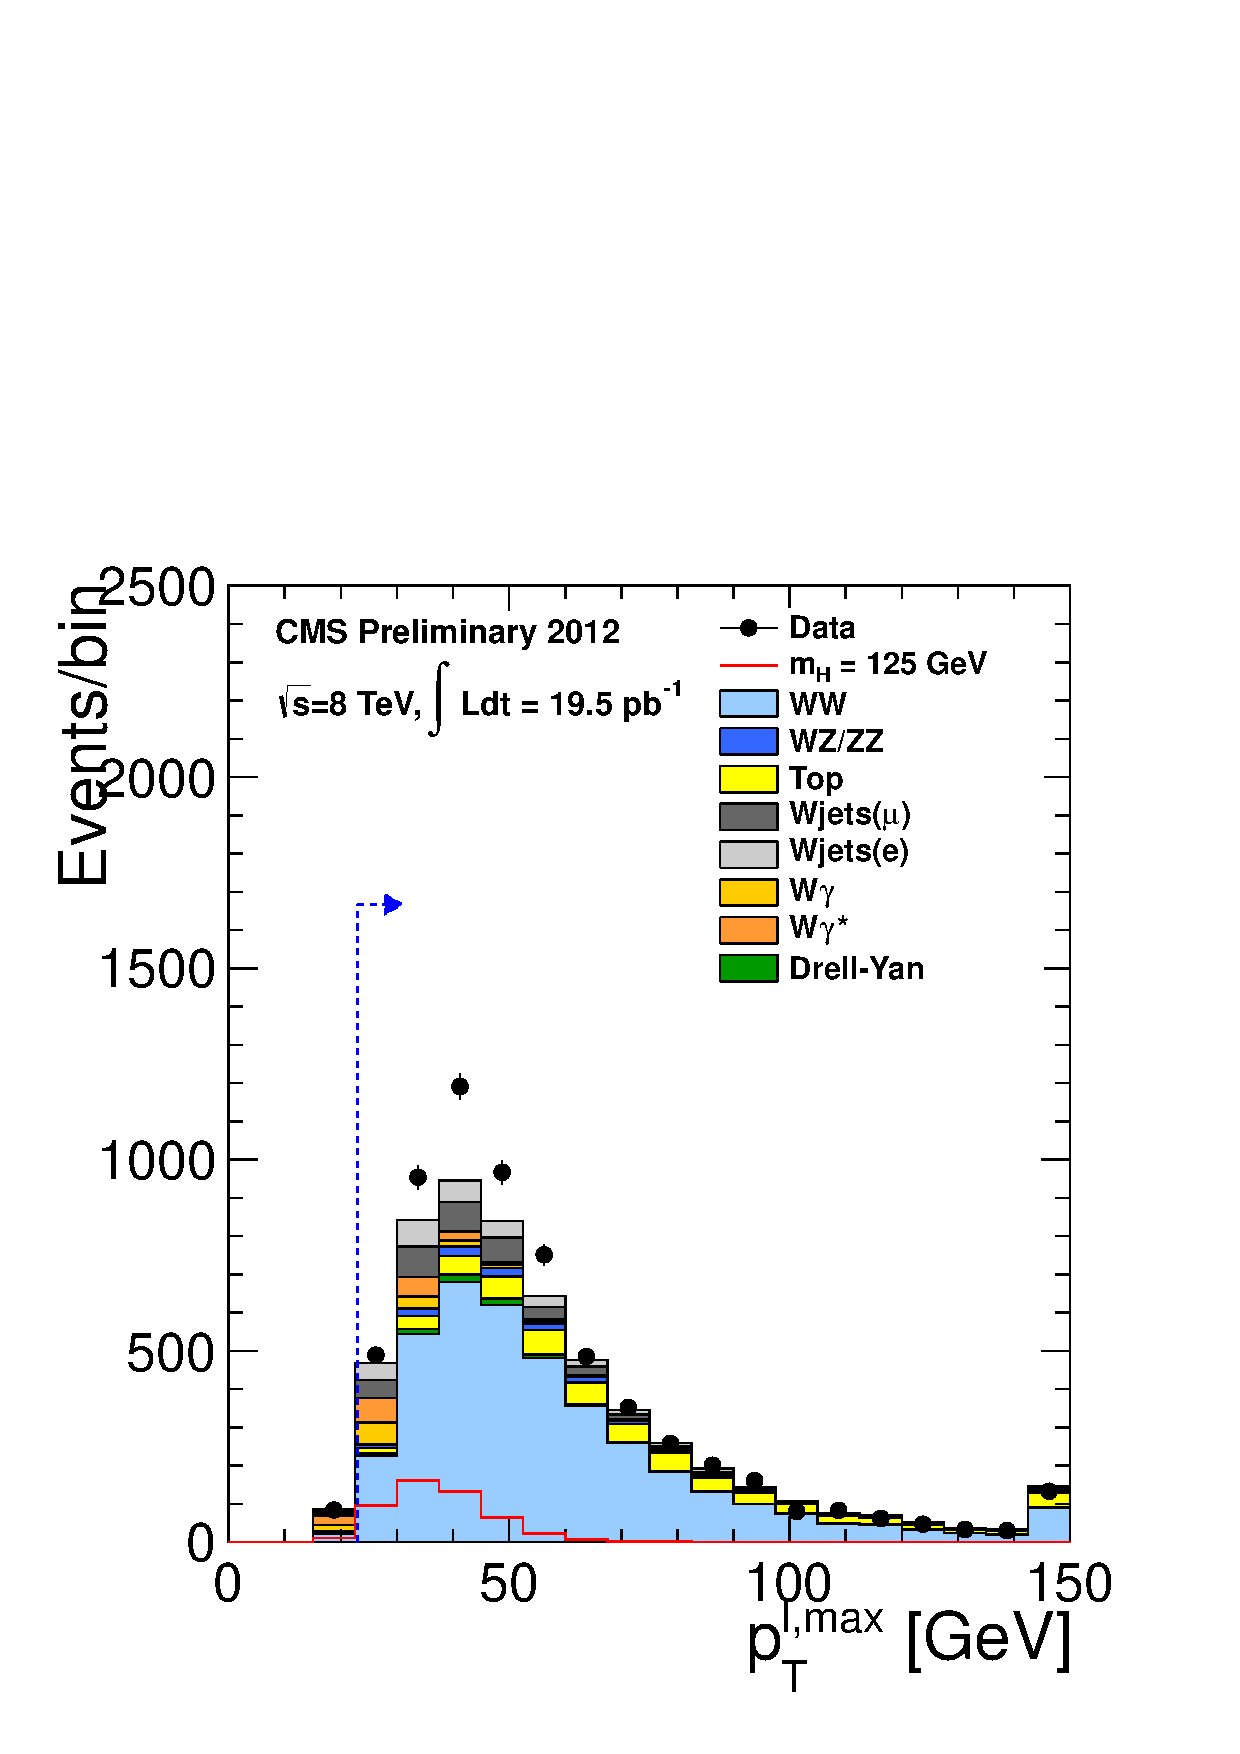
\includegraphics[width=0.45\textwidth]{figures/hww_analysis16_125_ALL_of_0j_pt1.pdf}
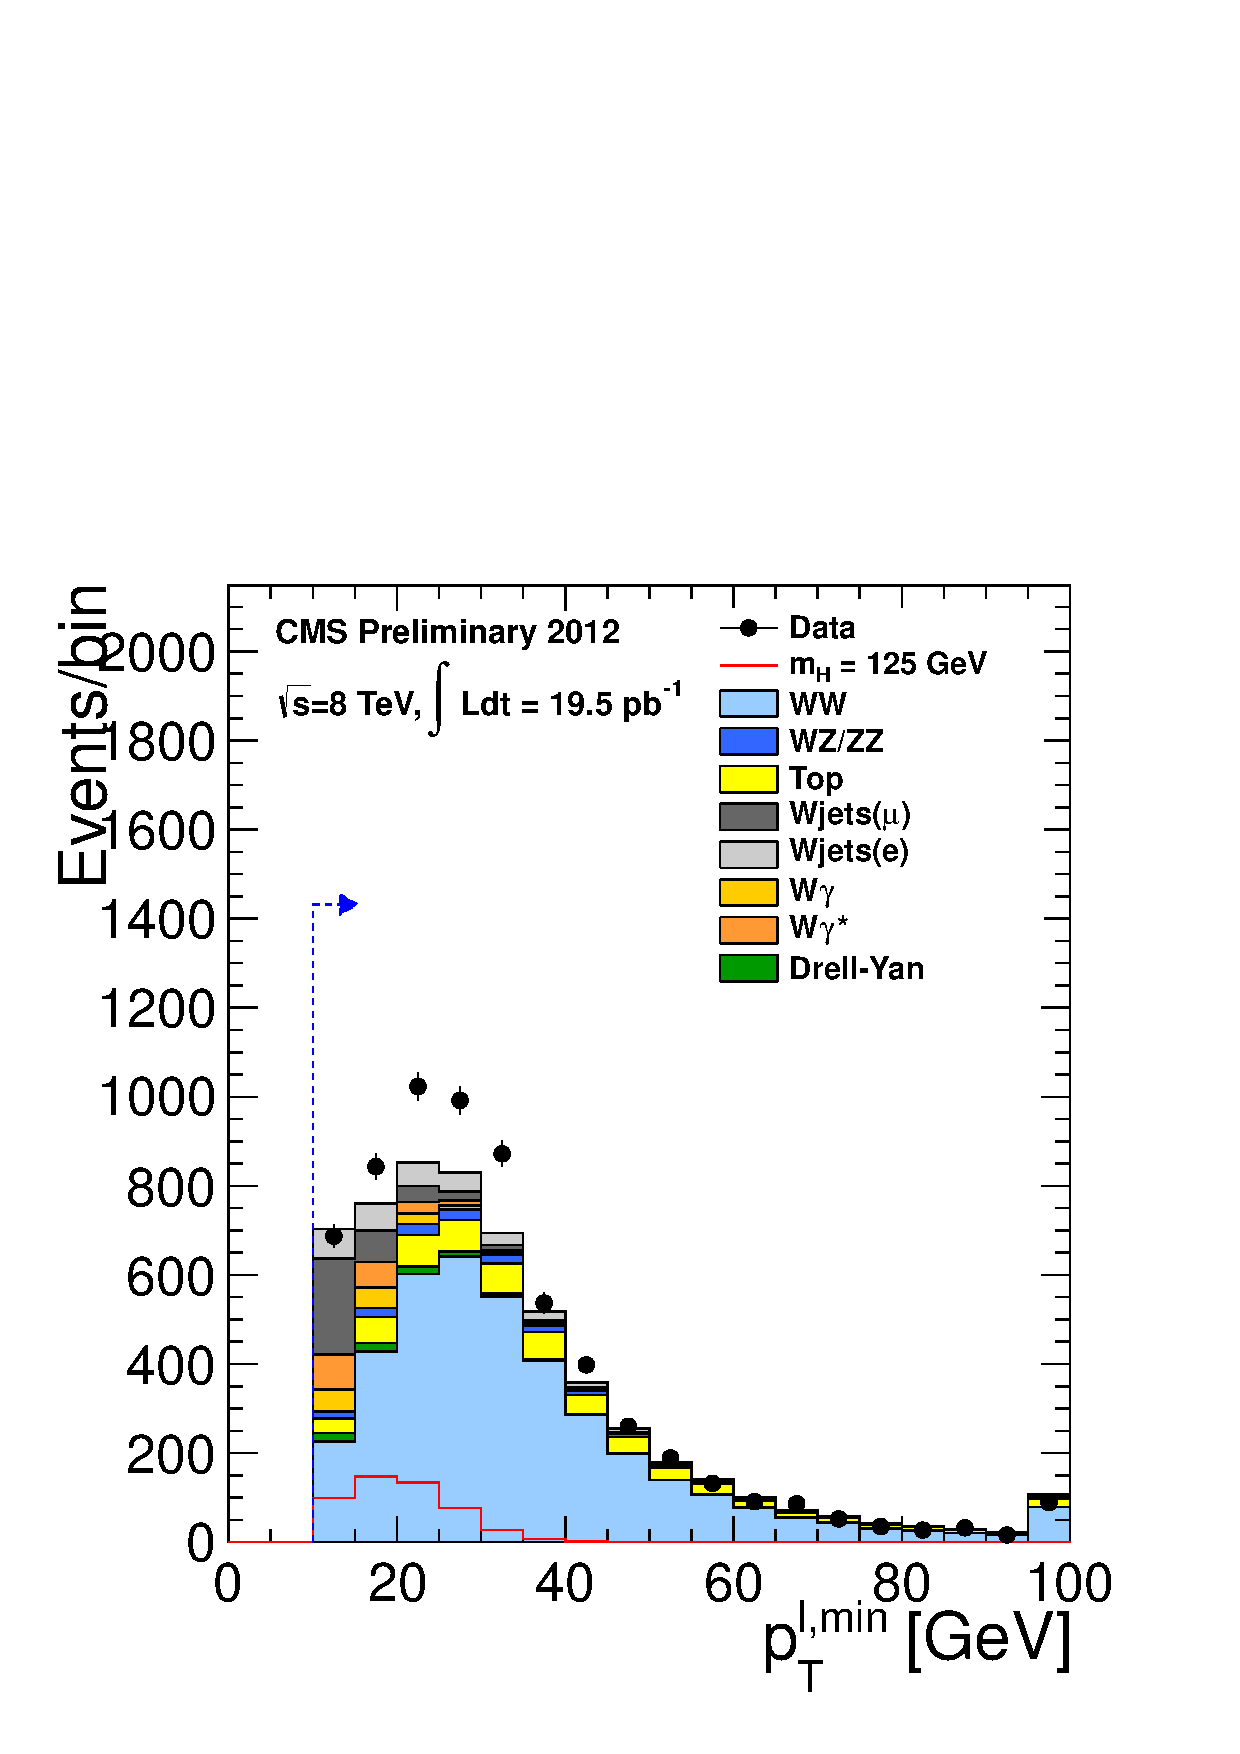
\includegraphics[width=0.45\textwidth]{figures/hww_analysis16_125_ALL_of_0j_pt2.pdf}
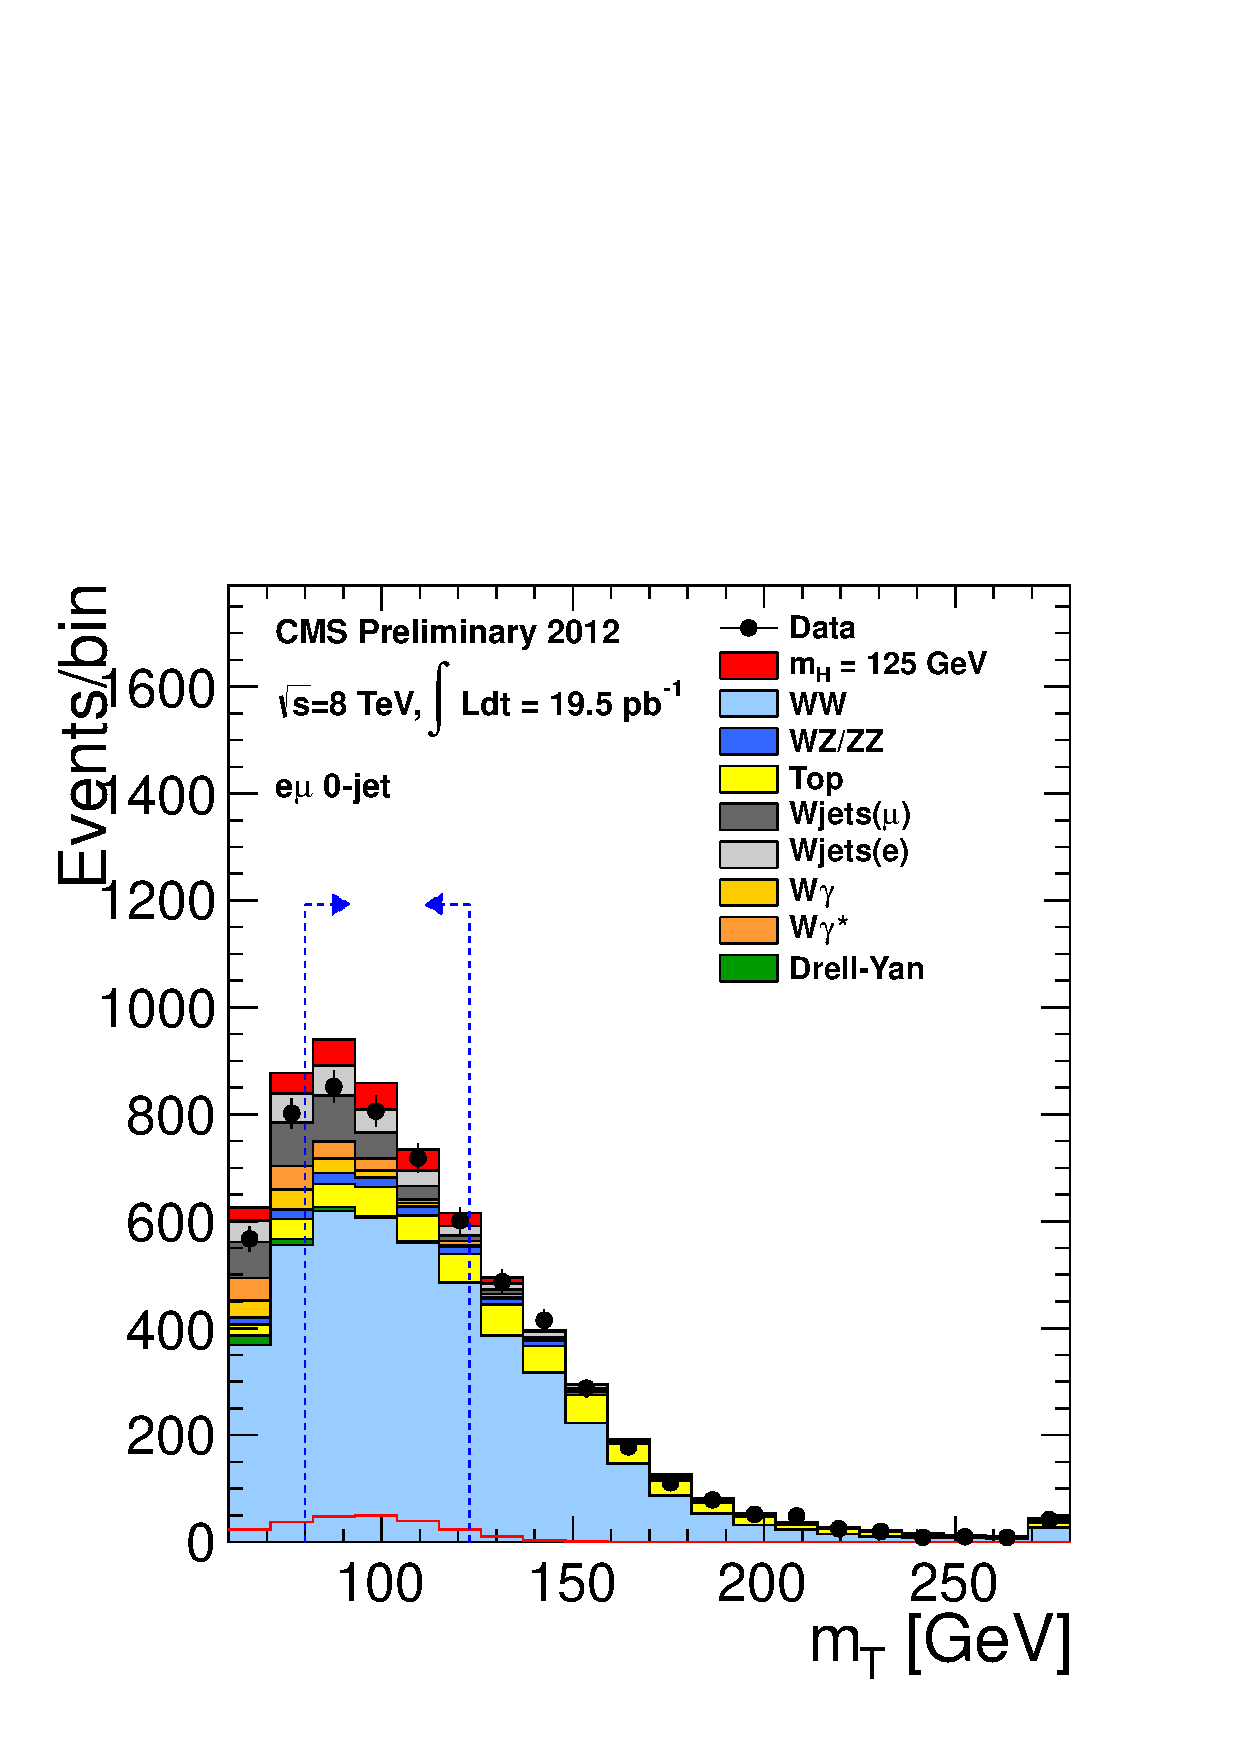
\includegraphics[width=0.45\textwidth]{figures/hww_analysis16_125_ALL_of_0j_mt.pdf}
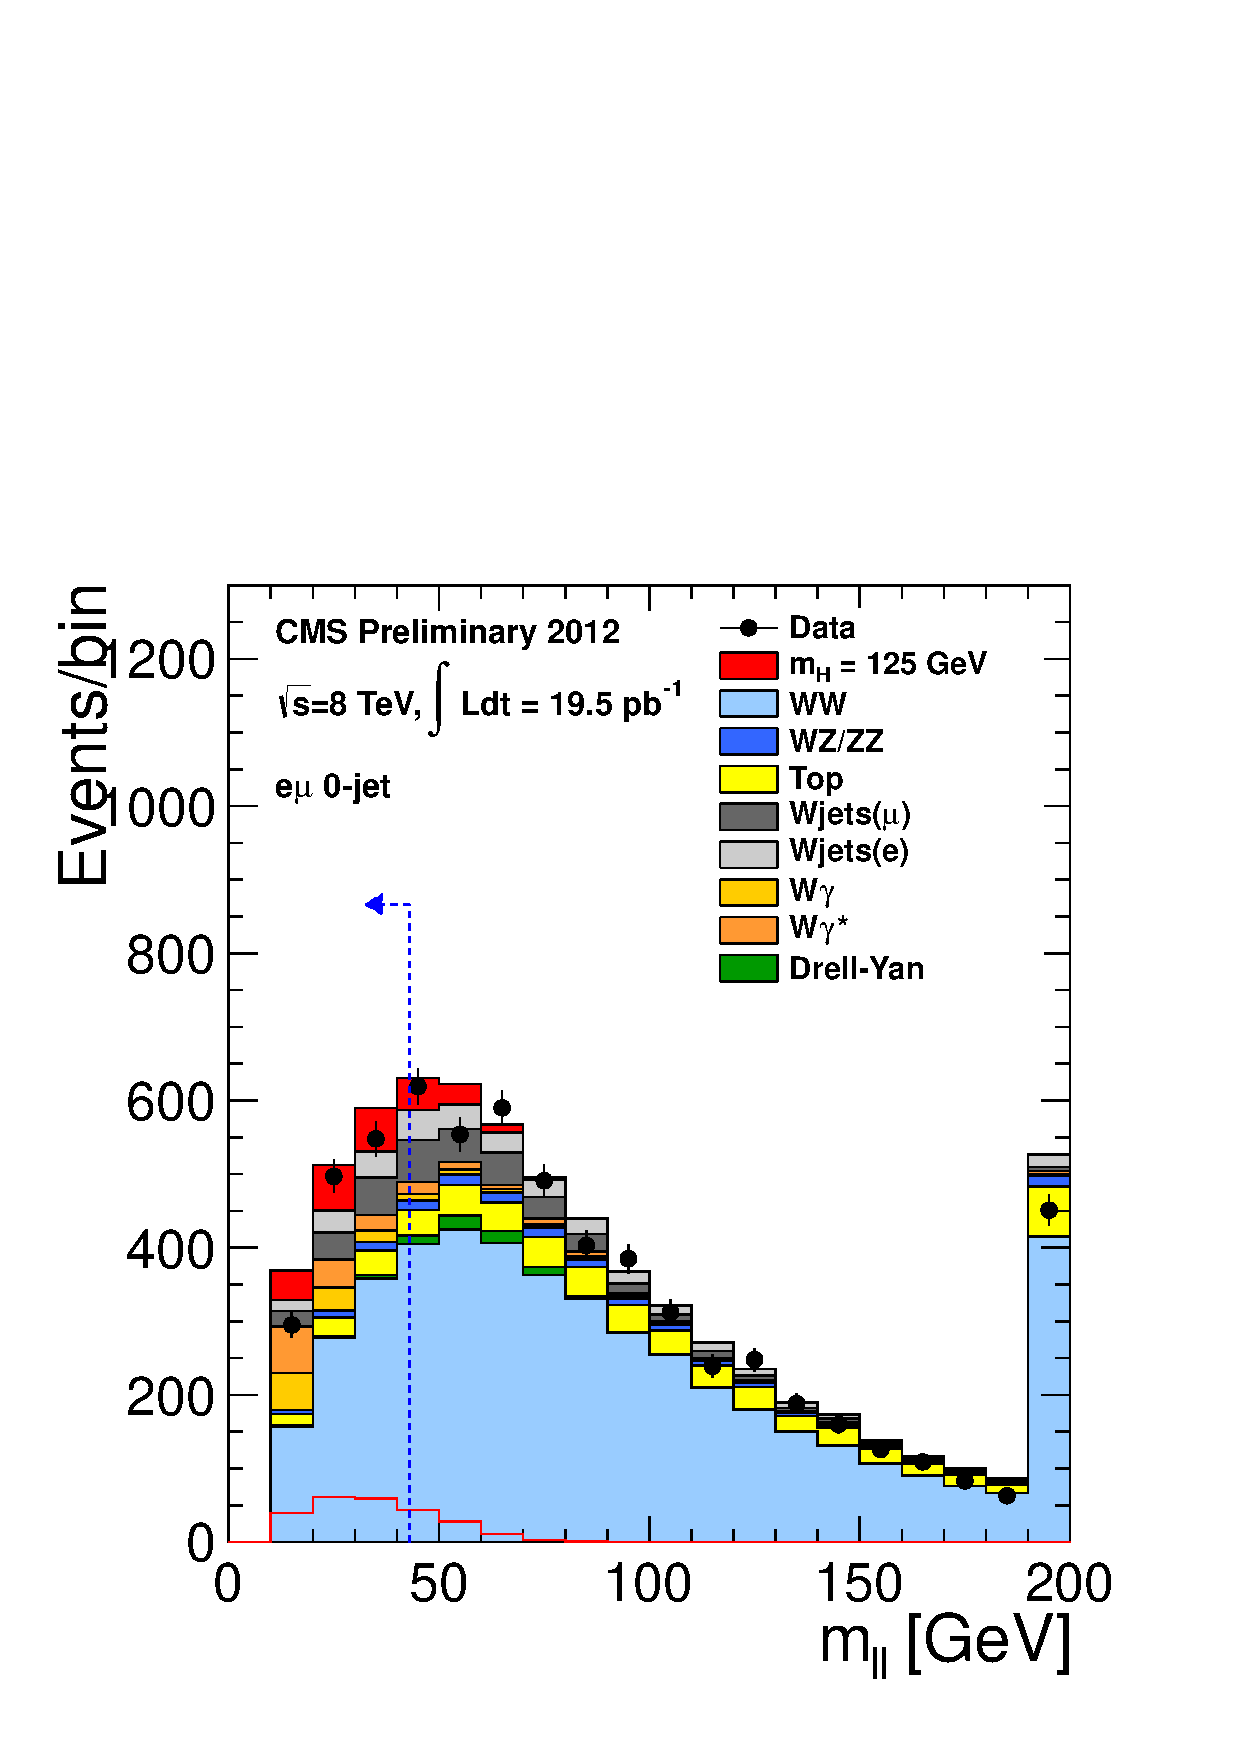
\includegraphics[width=0.45\textwidth]{figures/hww_analysis16_125_ALL_of_0j_mll.pdf}
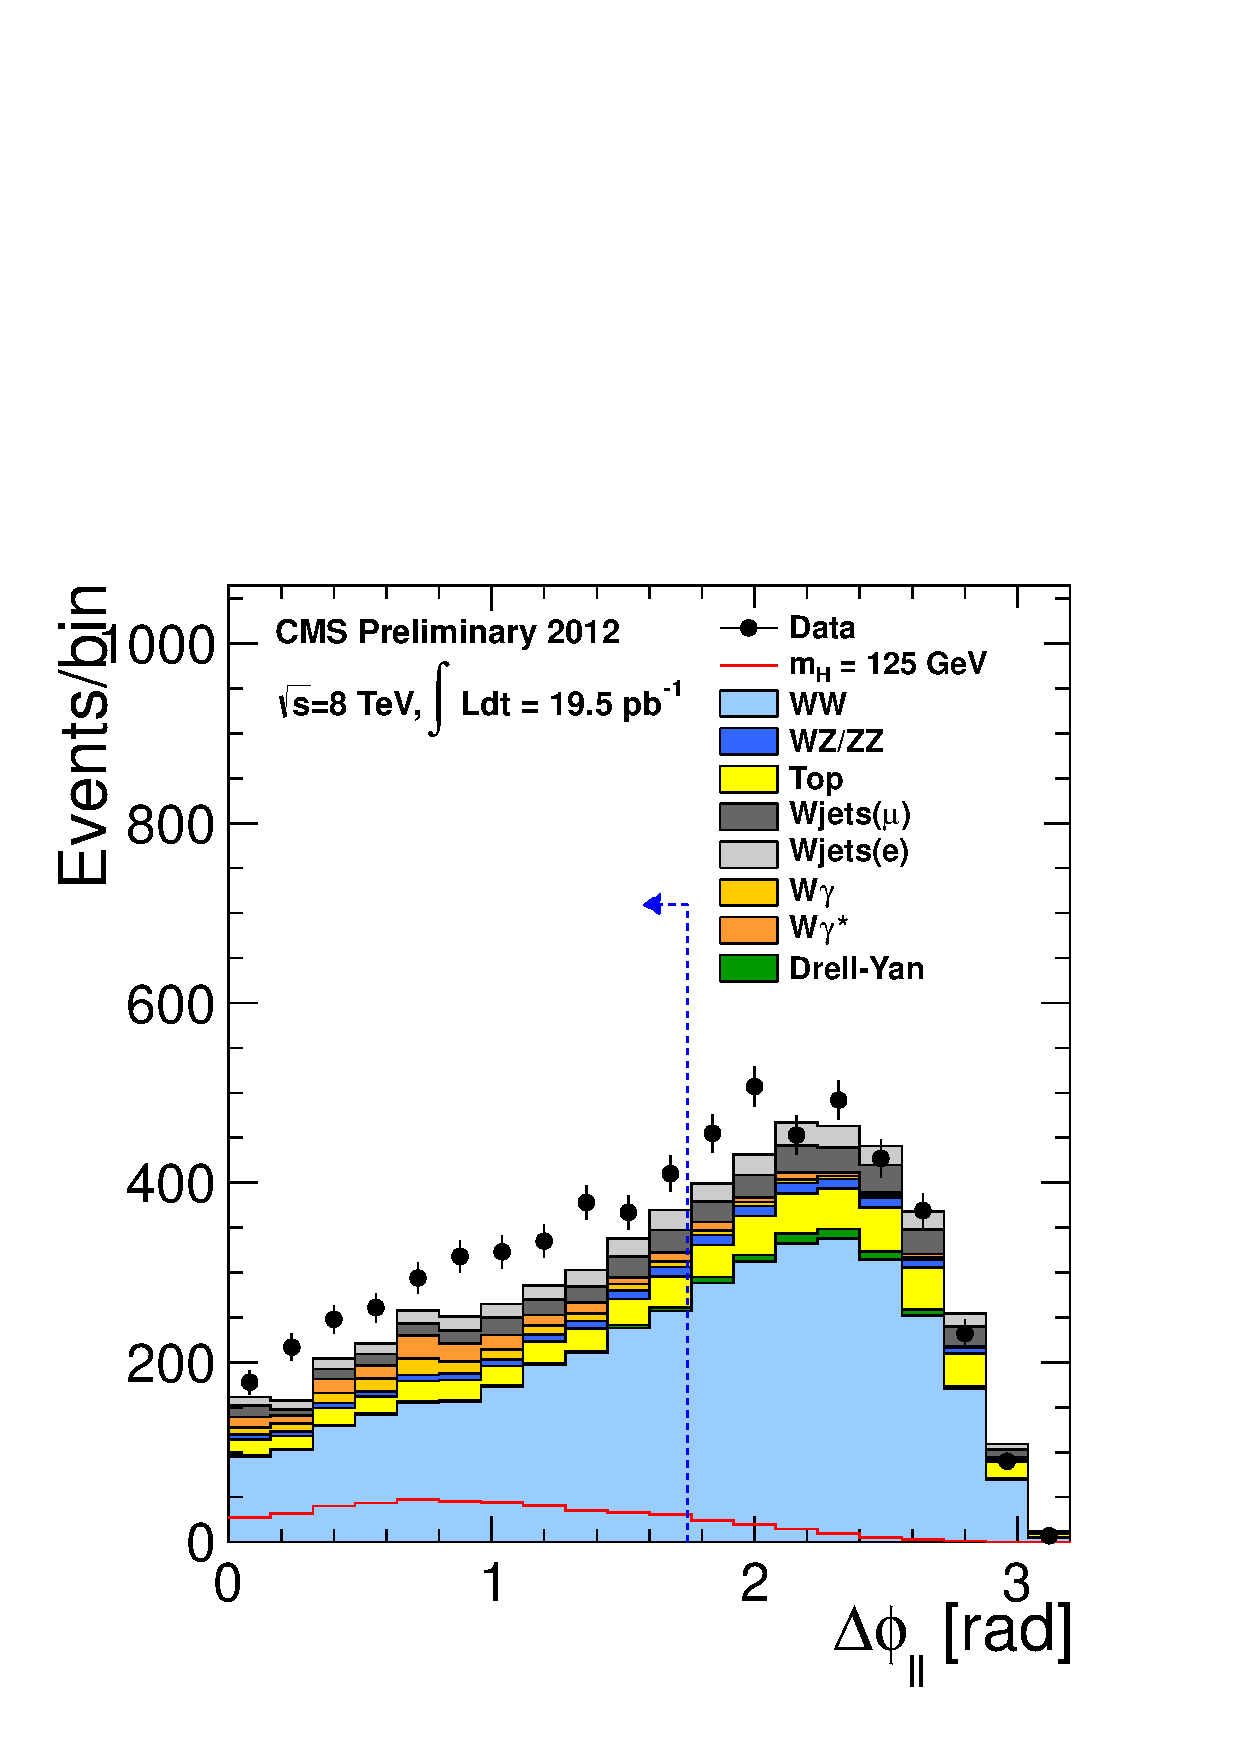
\includegraphics[width=0.45\textwidth]{figures/hww_analysis16_125_ALL_of_0j_dphi.pdf}
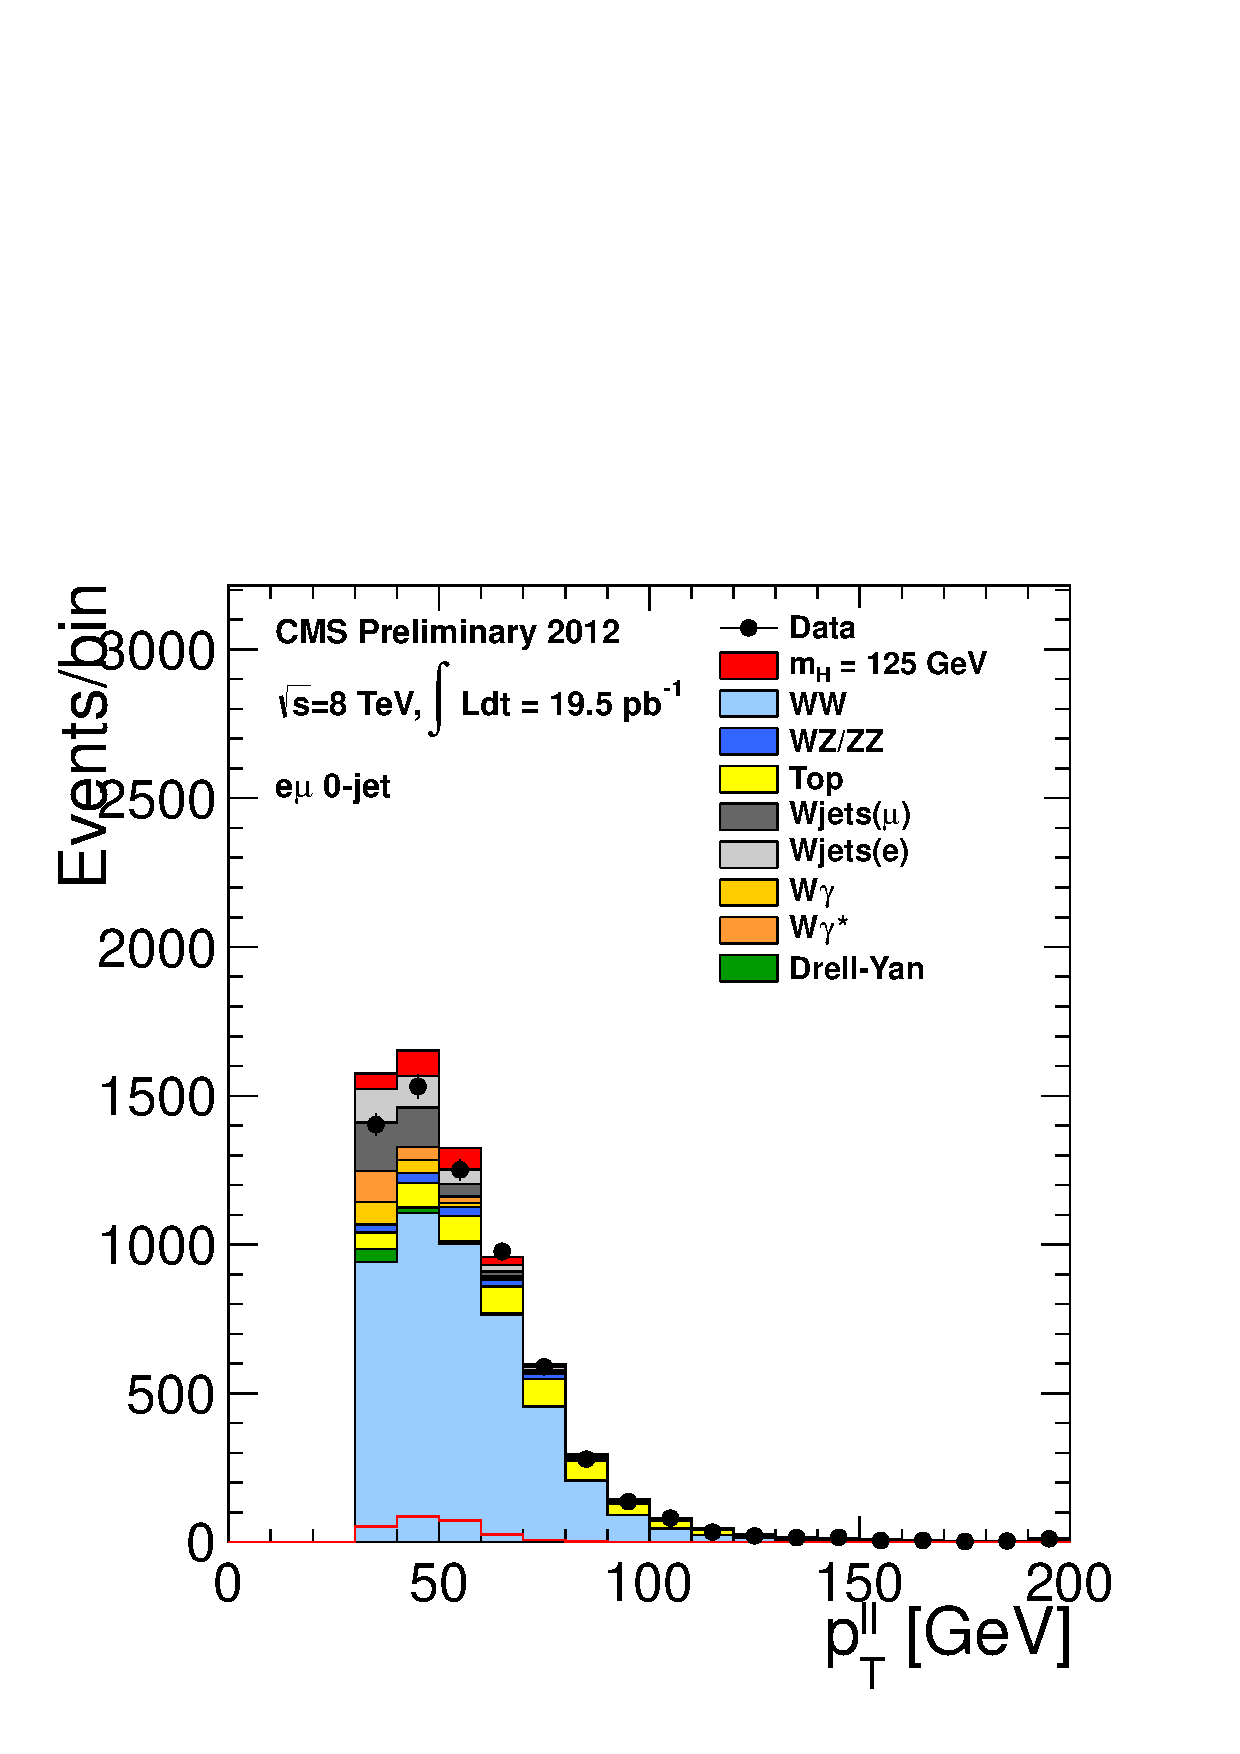
\includegraphics[width=0.45\textwidth]{figures/hww_analysis16_125_ALL_of_0j_ptll.pdf}
\caption{ WW-level plots in 0-jet \DF\ channel with \mHi=125~\GeV\ signal overlaid. 
Cuts for \mHi=125\GeV\ is shown with blue dotted lines and arrows. 
}
\label{fig:wwlevelmh125}
\end{figure}

% WW-level mH = 160 GeV
\begin{figure}[htp]
\centering
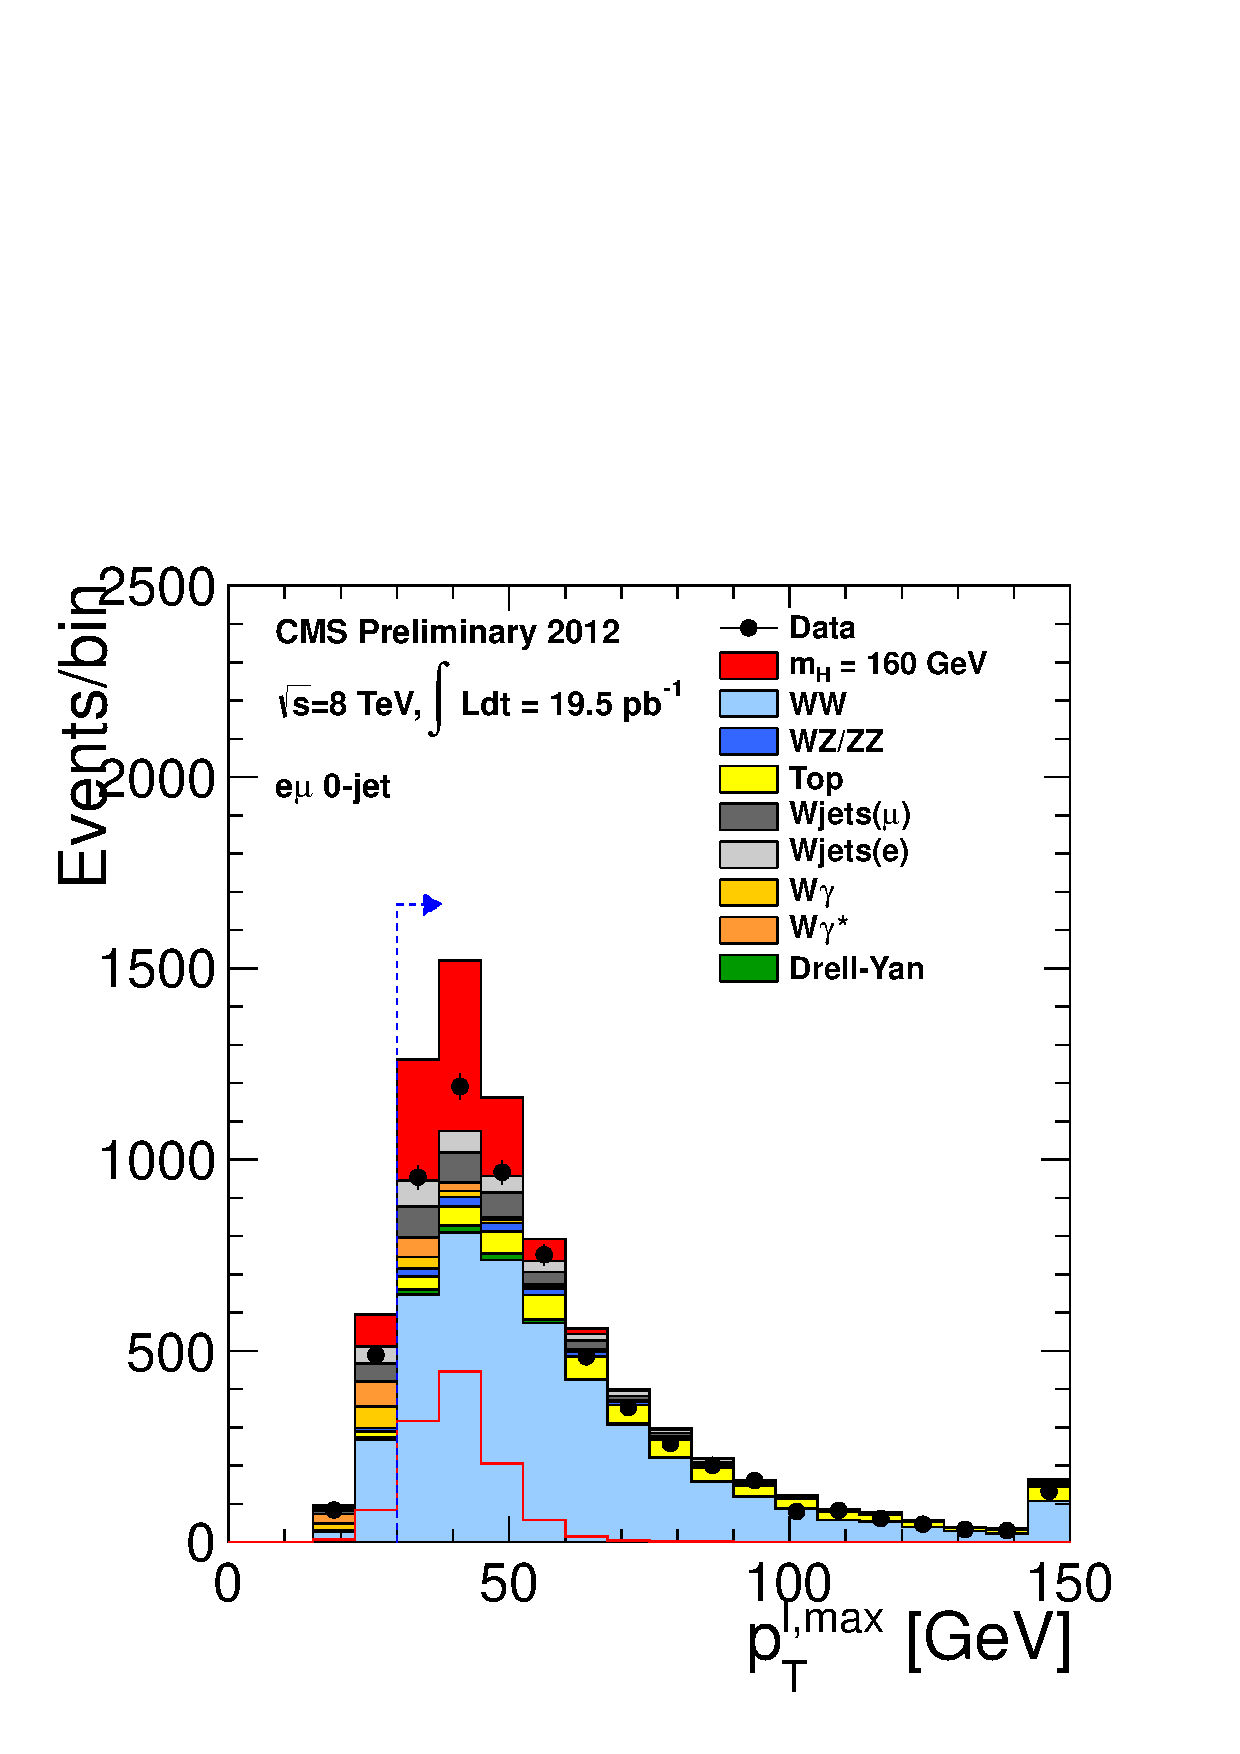
\includegraphics[width=0.45\textwidth]{figures/hww_analysis16_160_ALL_of_0j_pt1.pdf}
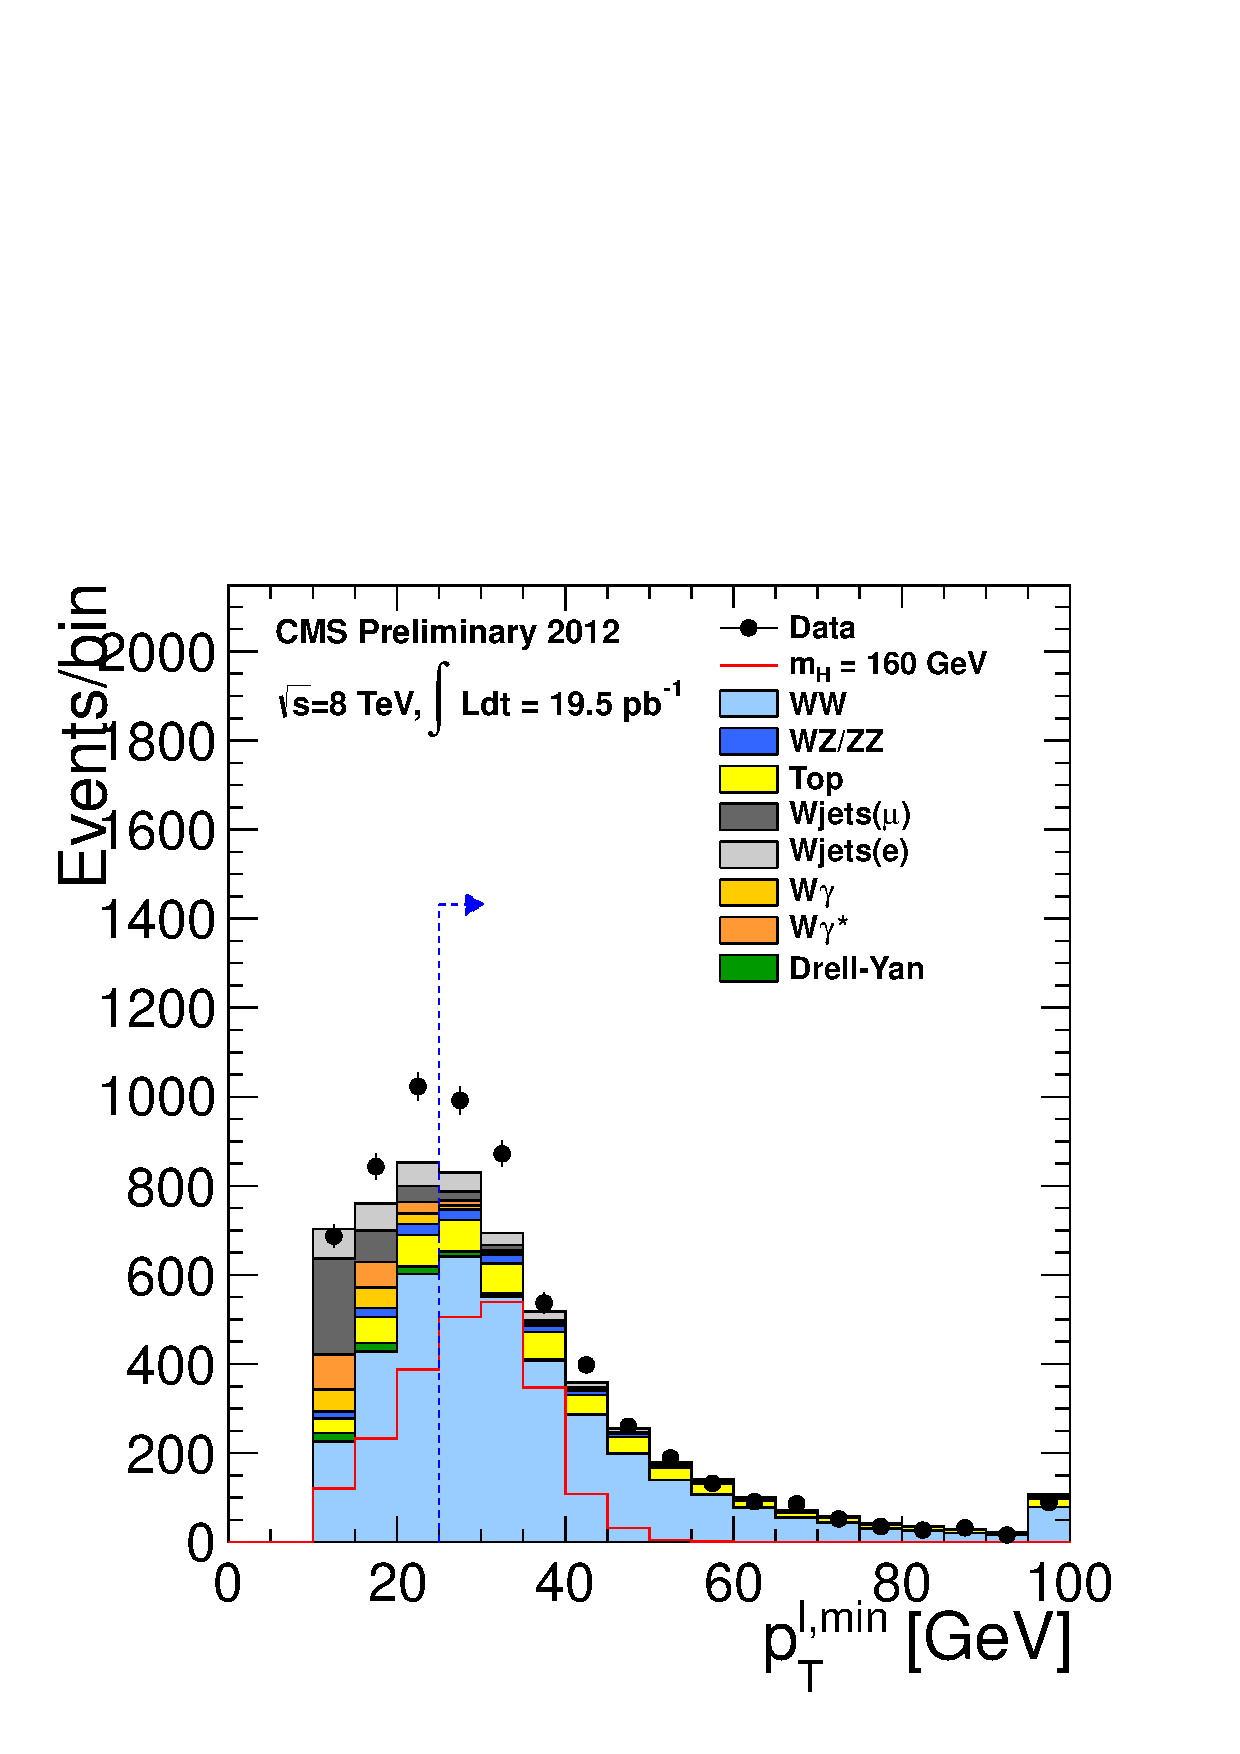
\includegraphics[width=0.45\textwidth]{figures/hww_analysis16_160_ALL_of_0j_pt2.pdf}
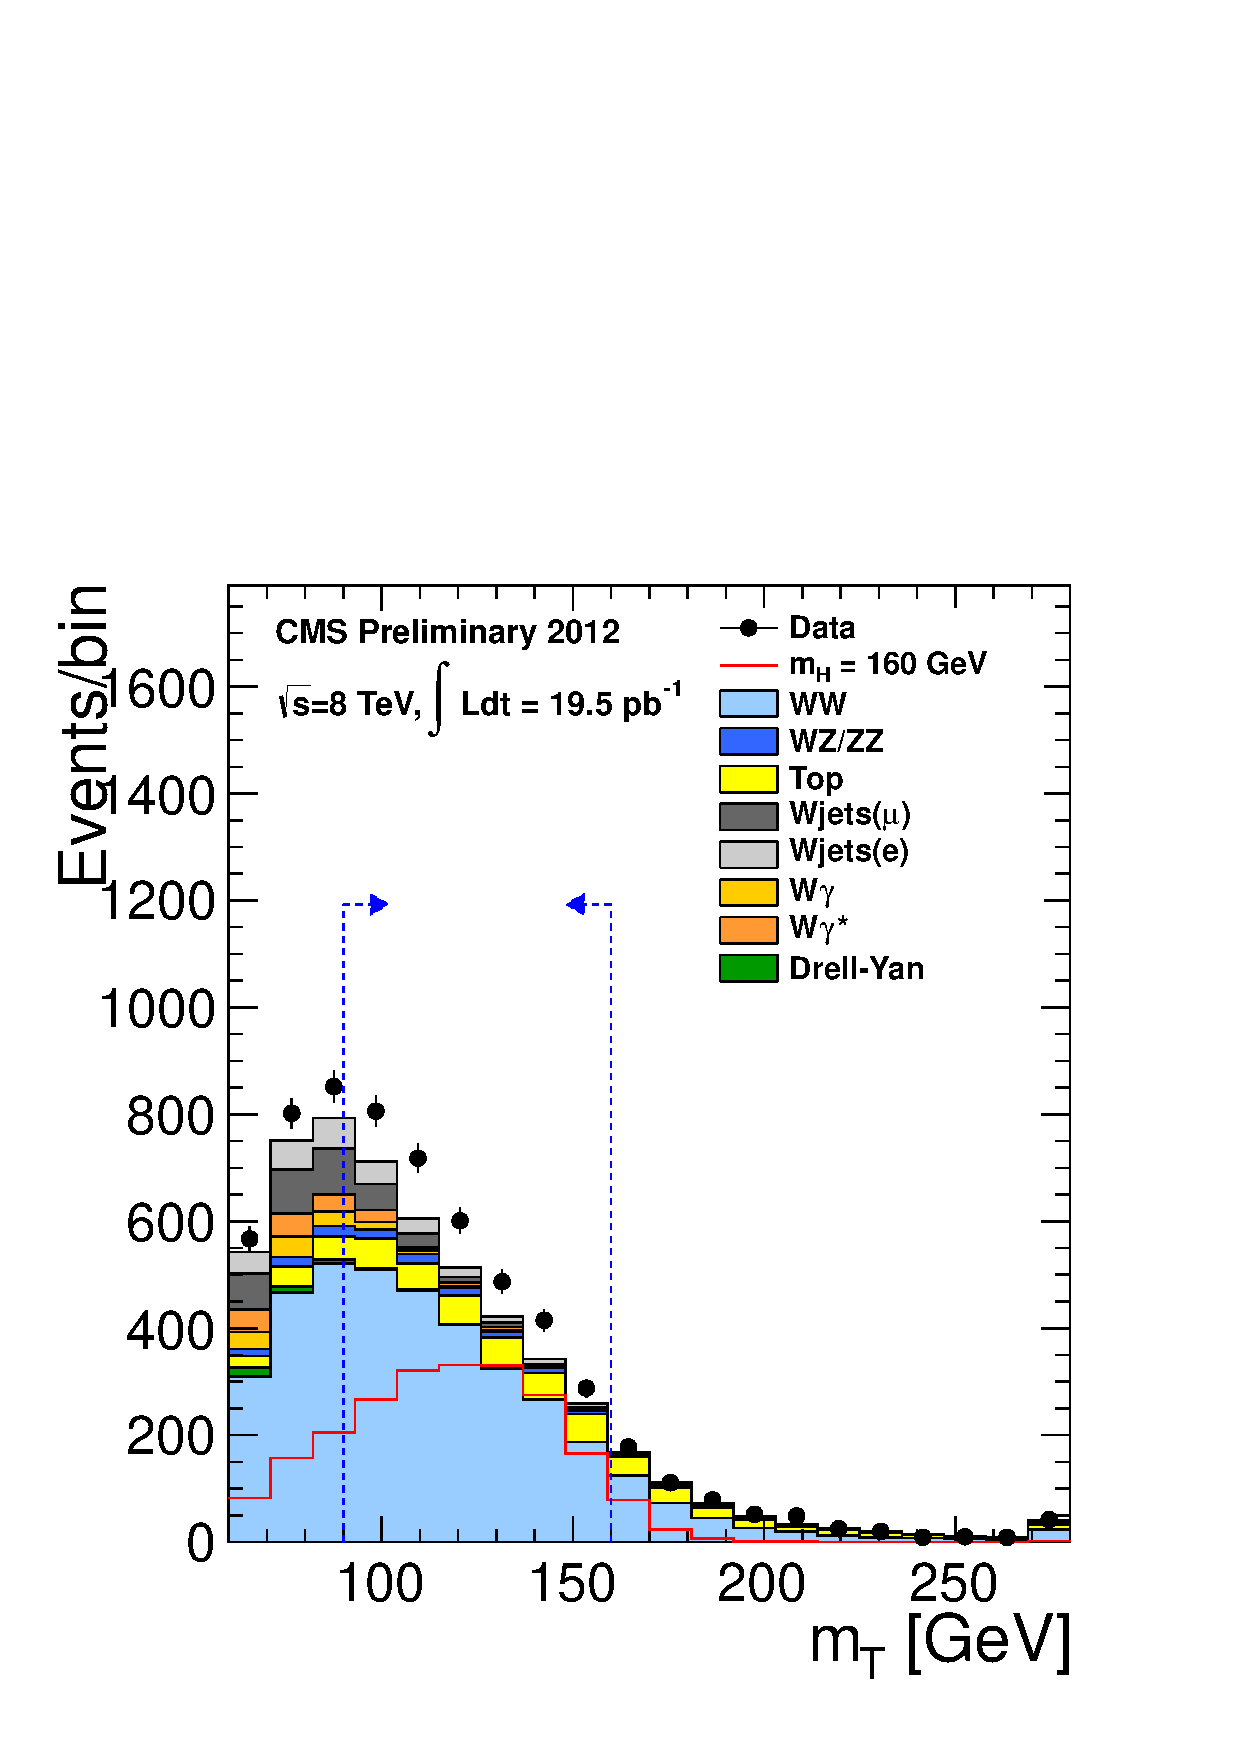
\includegraphics[width=0.45\textwidth]{figures/hww_analysis16_160_ALL_of_0j_mt.pdf}
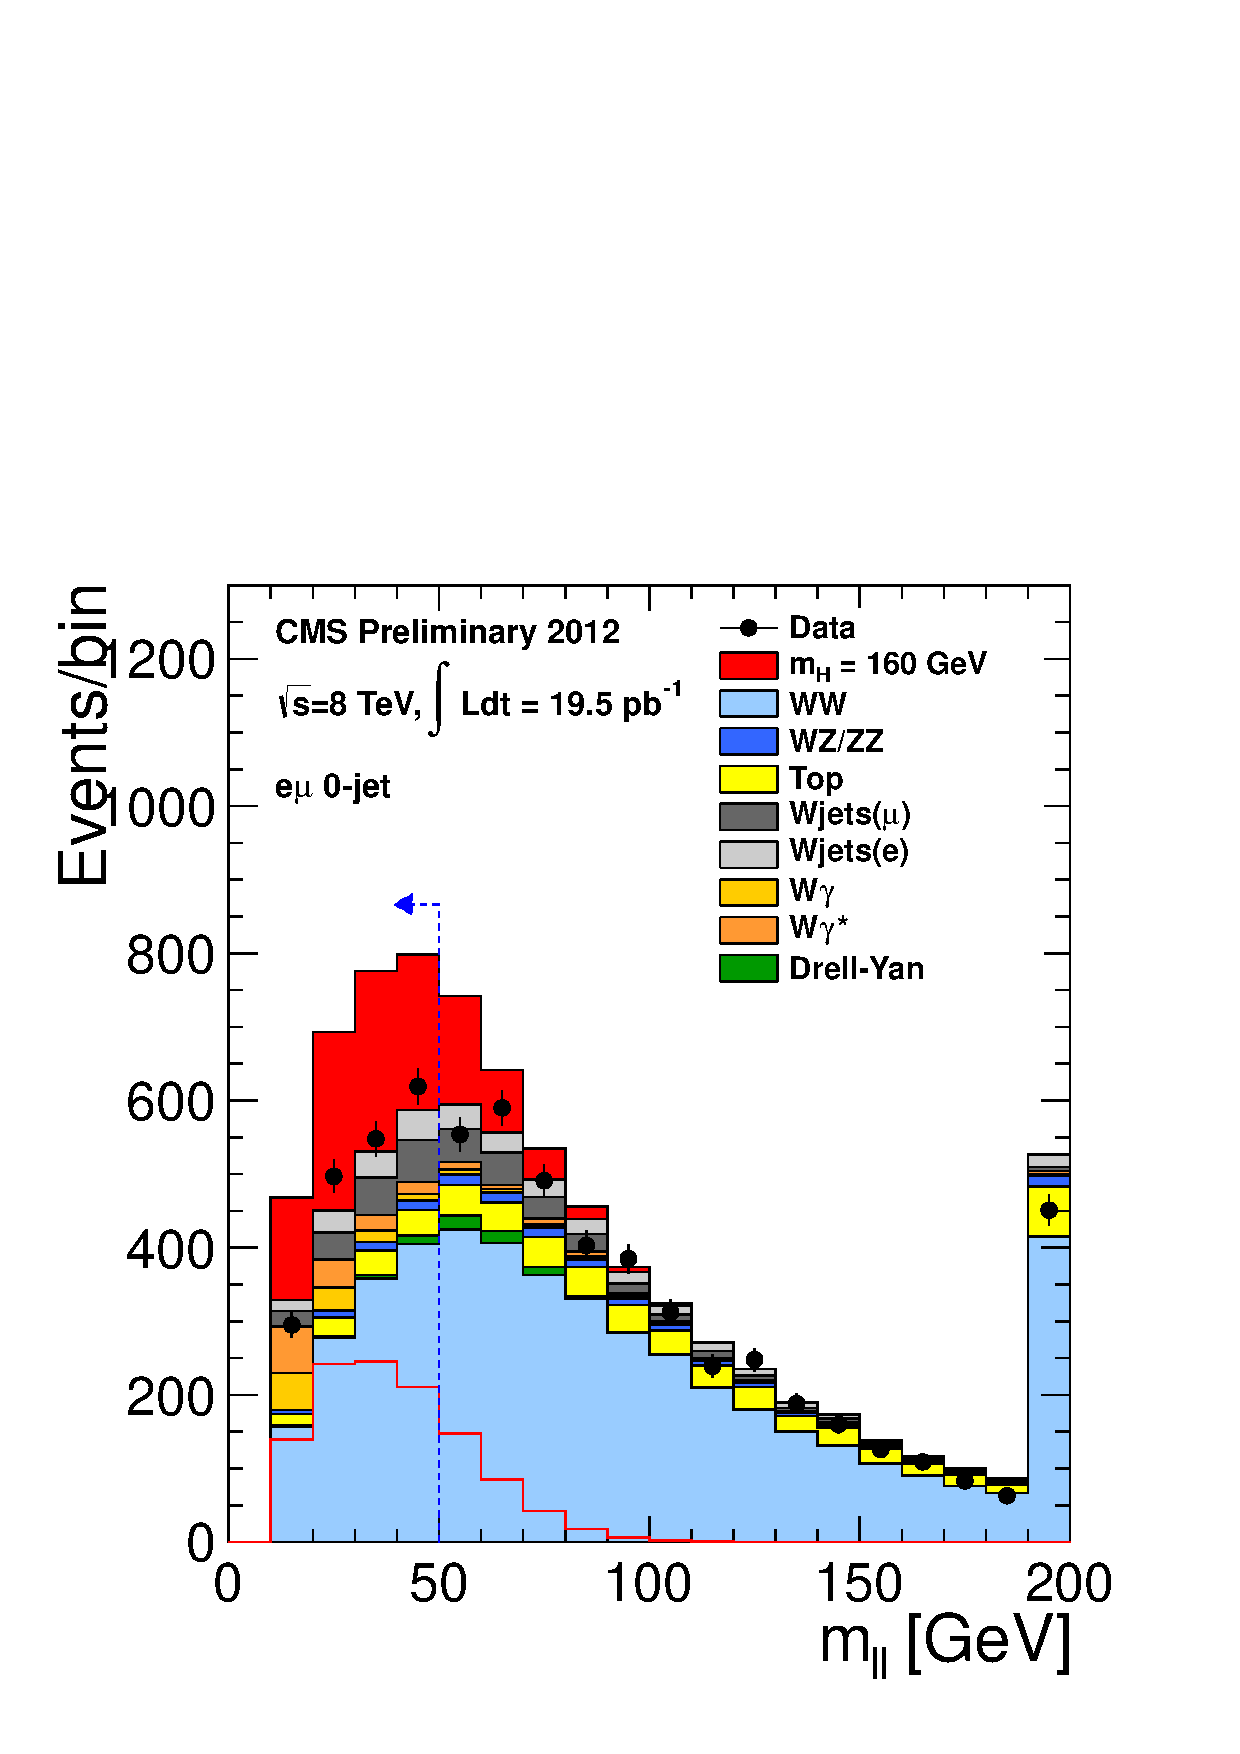
\includegraphics[width=0.45\textwidth]{figures/hww_analysis16_160_ALL_of_0j_mll.pdf}
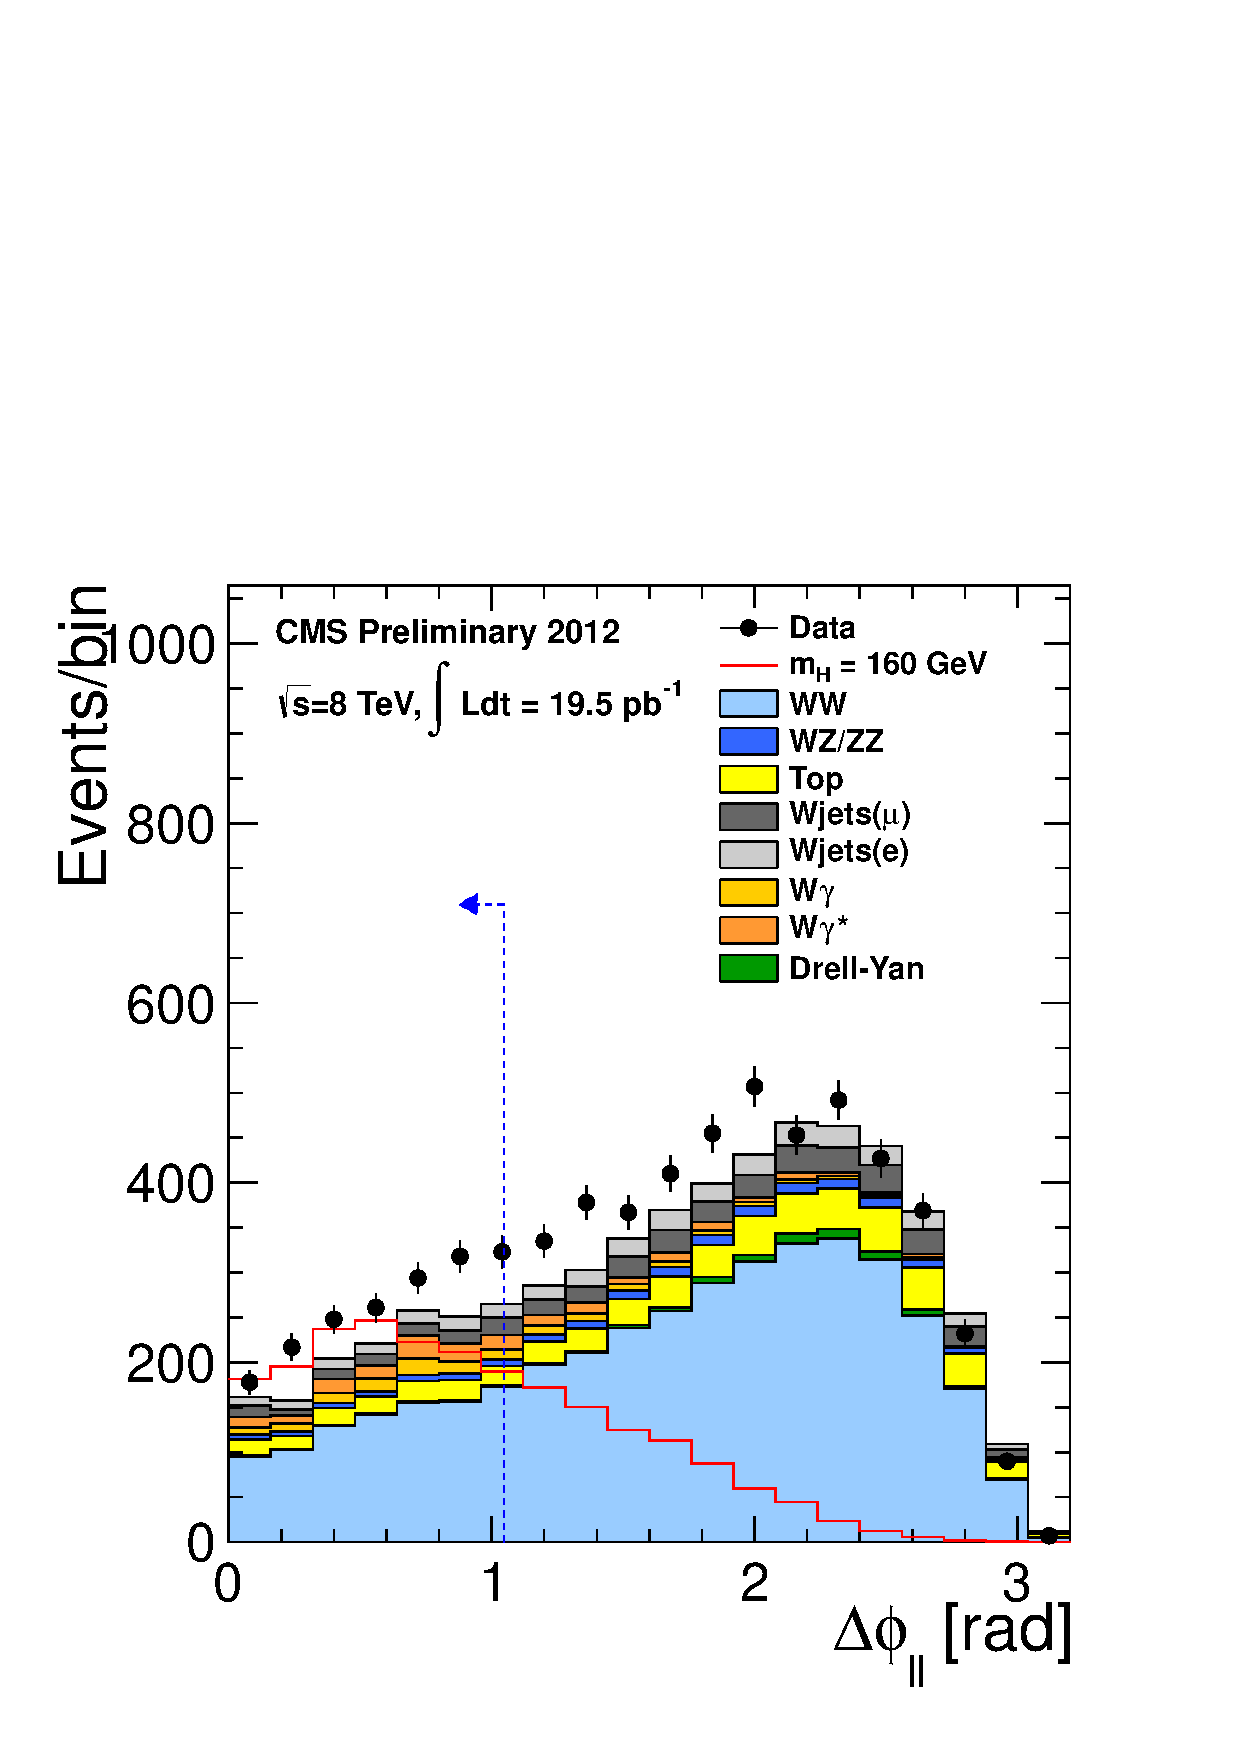
\includegraphics[width=0.45\textwidth]{figures/hww_analysis16_160_ALL_of_0j_dphi.pdf}
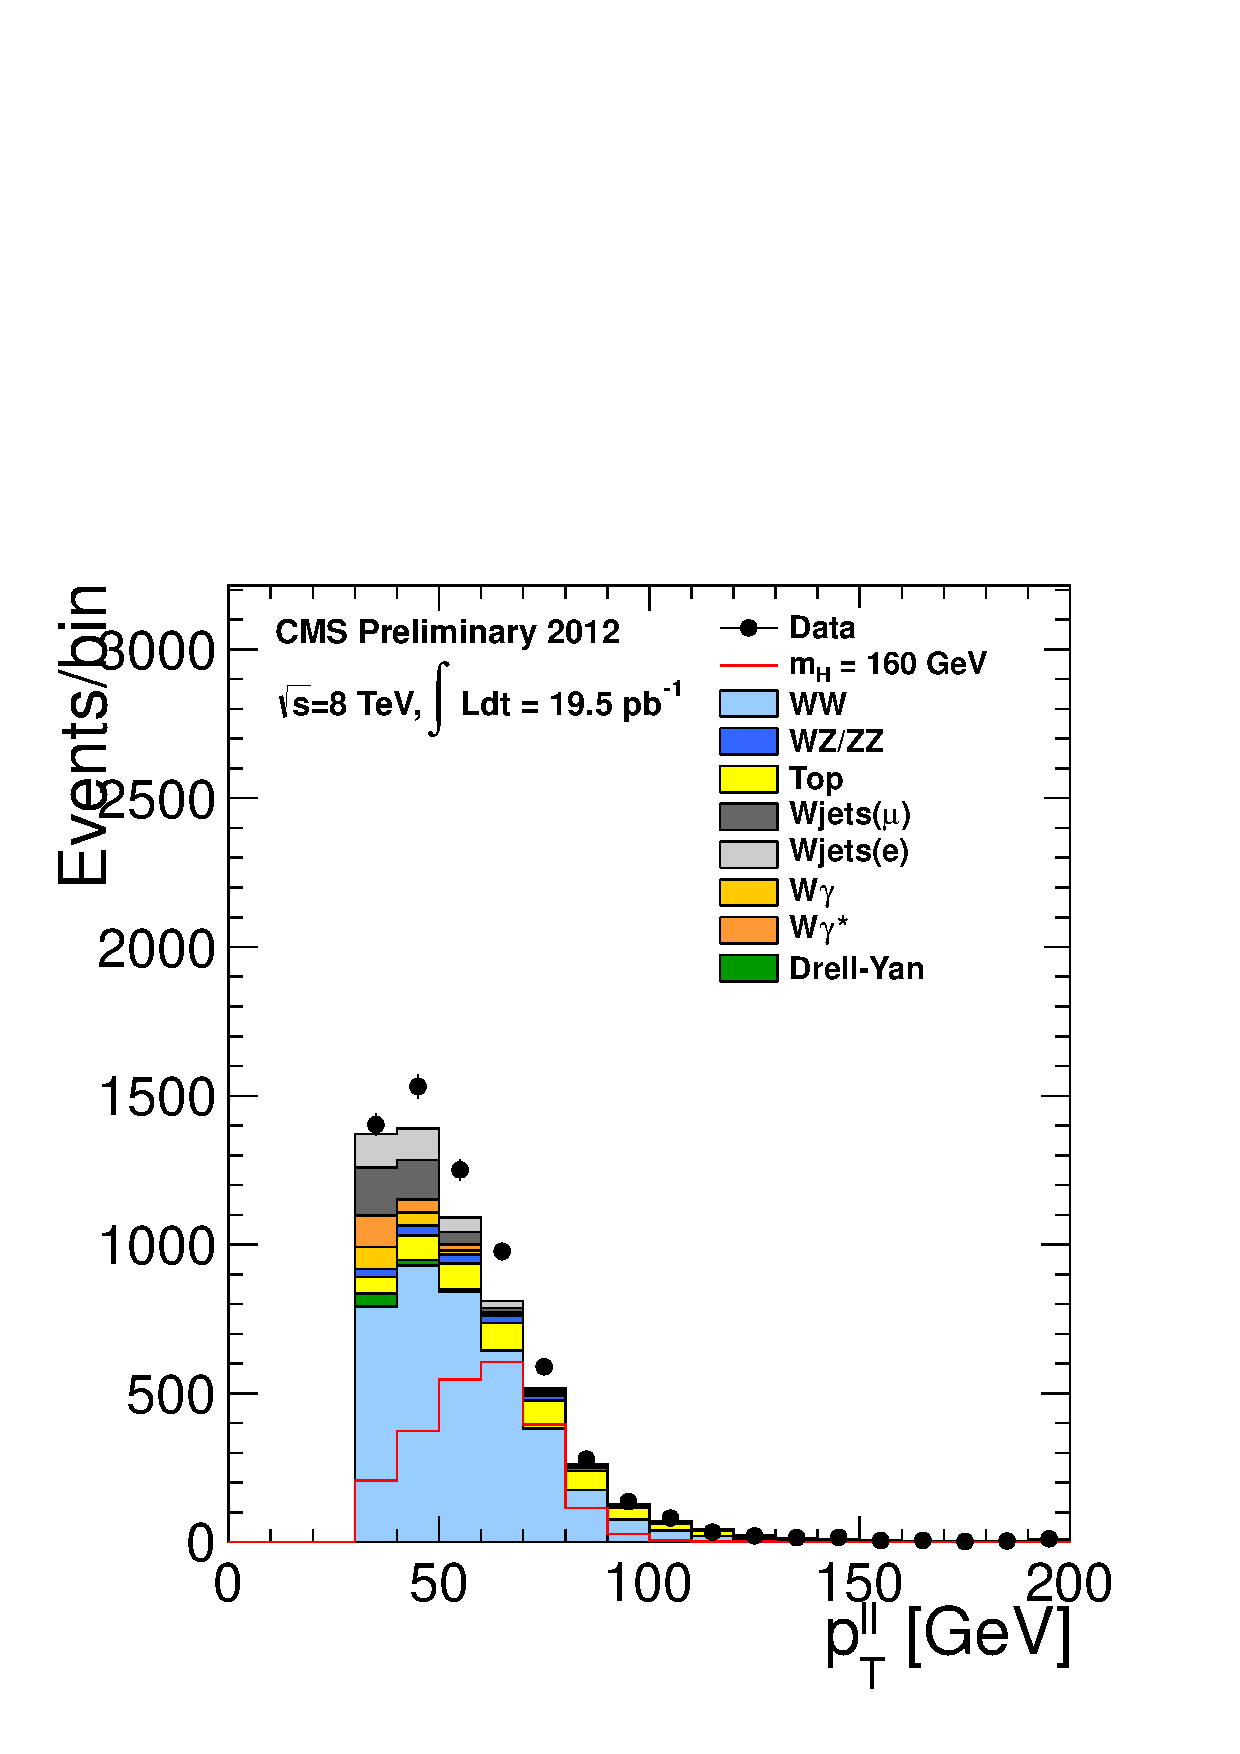
\includegraphics[width=0.45\textwidth]{figures/hww_analysis16_160_ALL_of_0j_ptll.pdf}
\caption{ WW-level plots in 0-jet \DF\ channel with \mHi=160~\GeV\ signal overlaid. 
Cuts for \mHi=160\GeV\ is shown with blue dotted lines and arrows. 
}
\label{fig:wwlevelmh160}
\end{figure}

% WW-level mH = 200 GeV
\begin{figure}[htp]
\centering
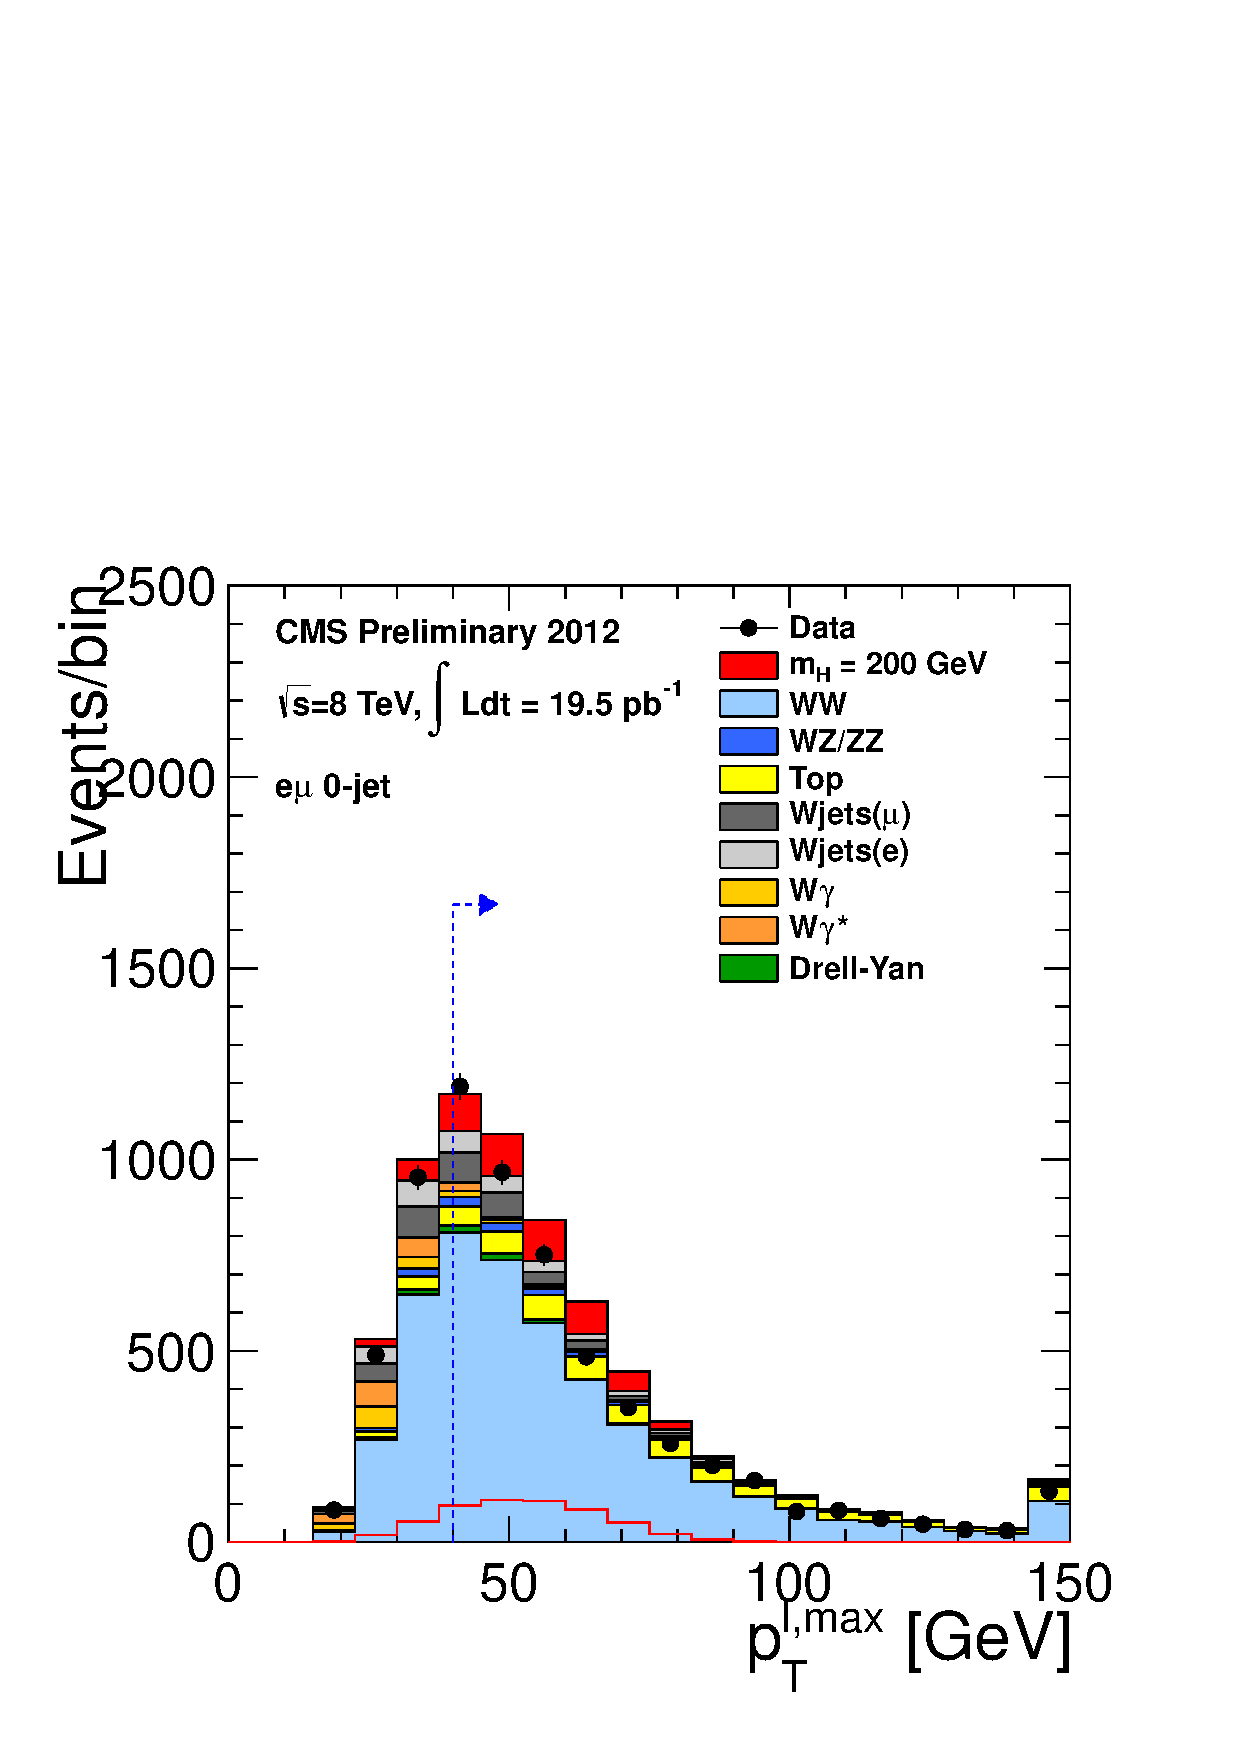
\includegraphics[width=0.45\textwidth]{figures/hww_analysis16_200_ALL_of_0j_pt1.pdf}
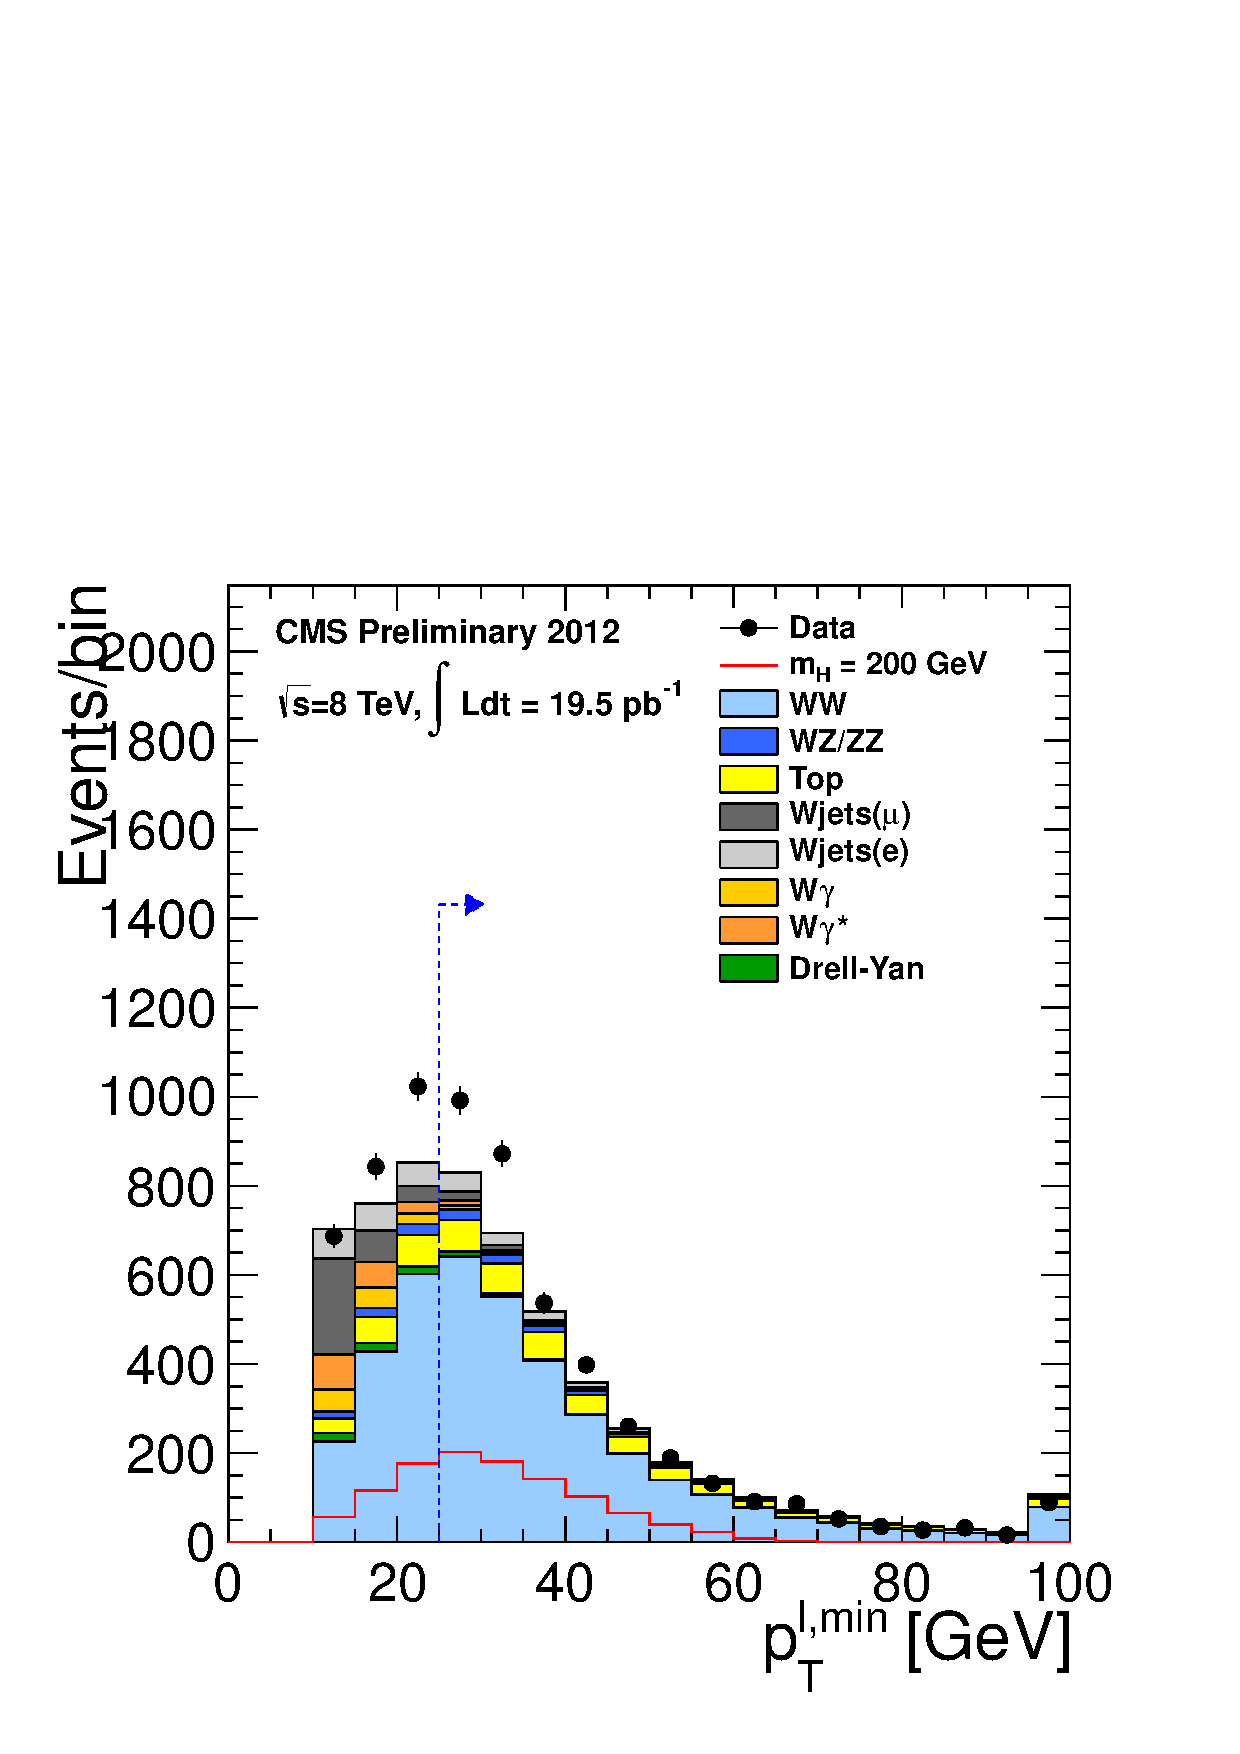
\includegraphics[width=0.45\textwidth]{figures/hww_analysis16_200_ALL_of_0j_pt2.pdf}
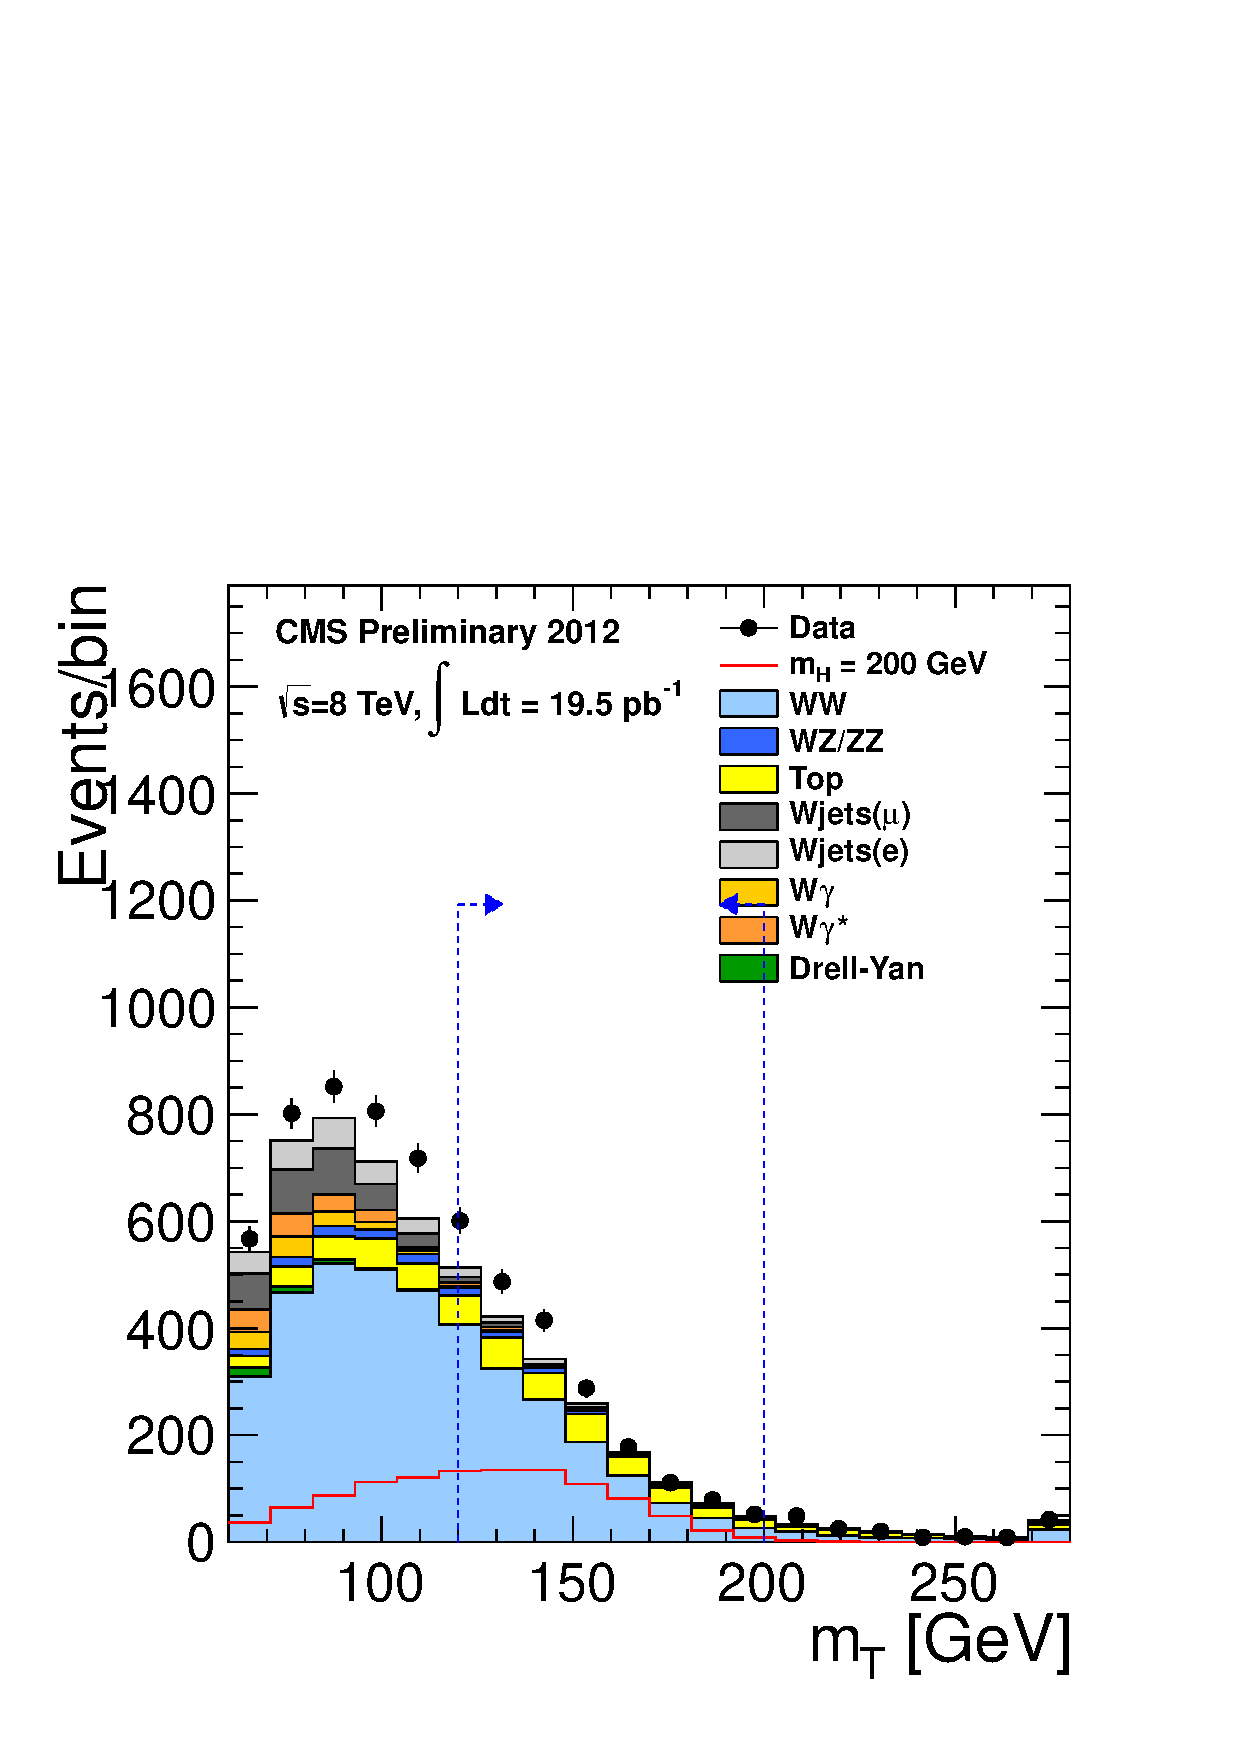
\includegraphics[width=0.45\textwidth]{figures/hww_analysis16_200_ALL_of_0j_mt.pdf}
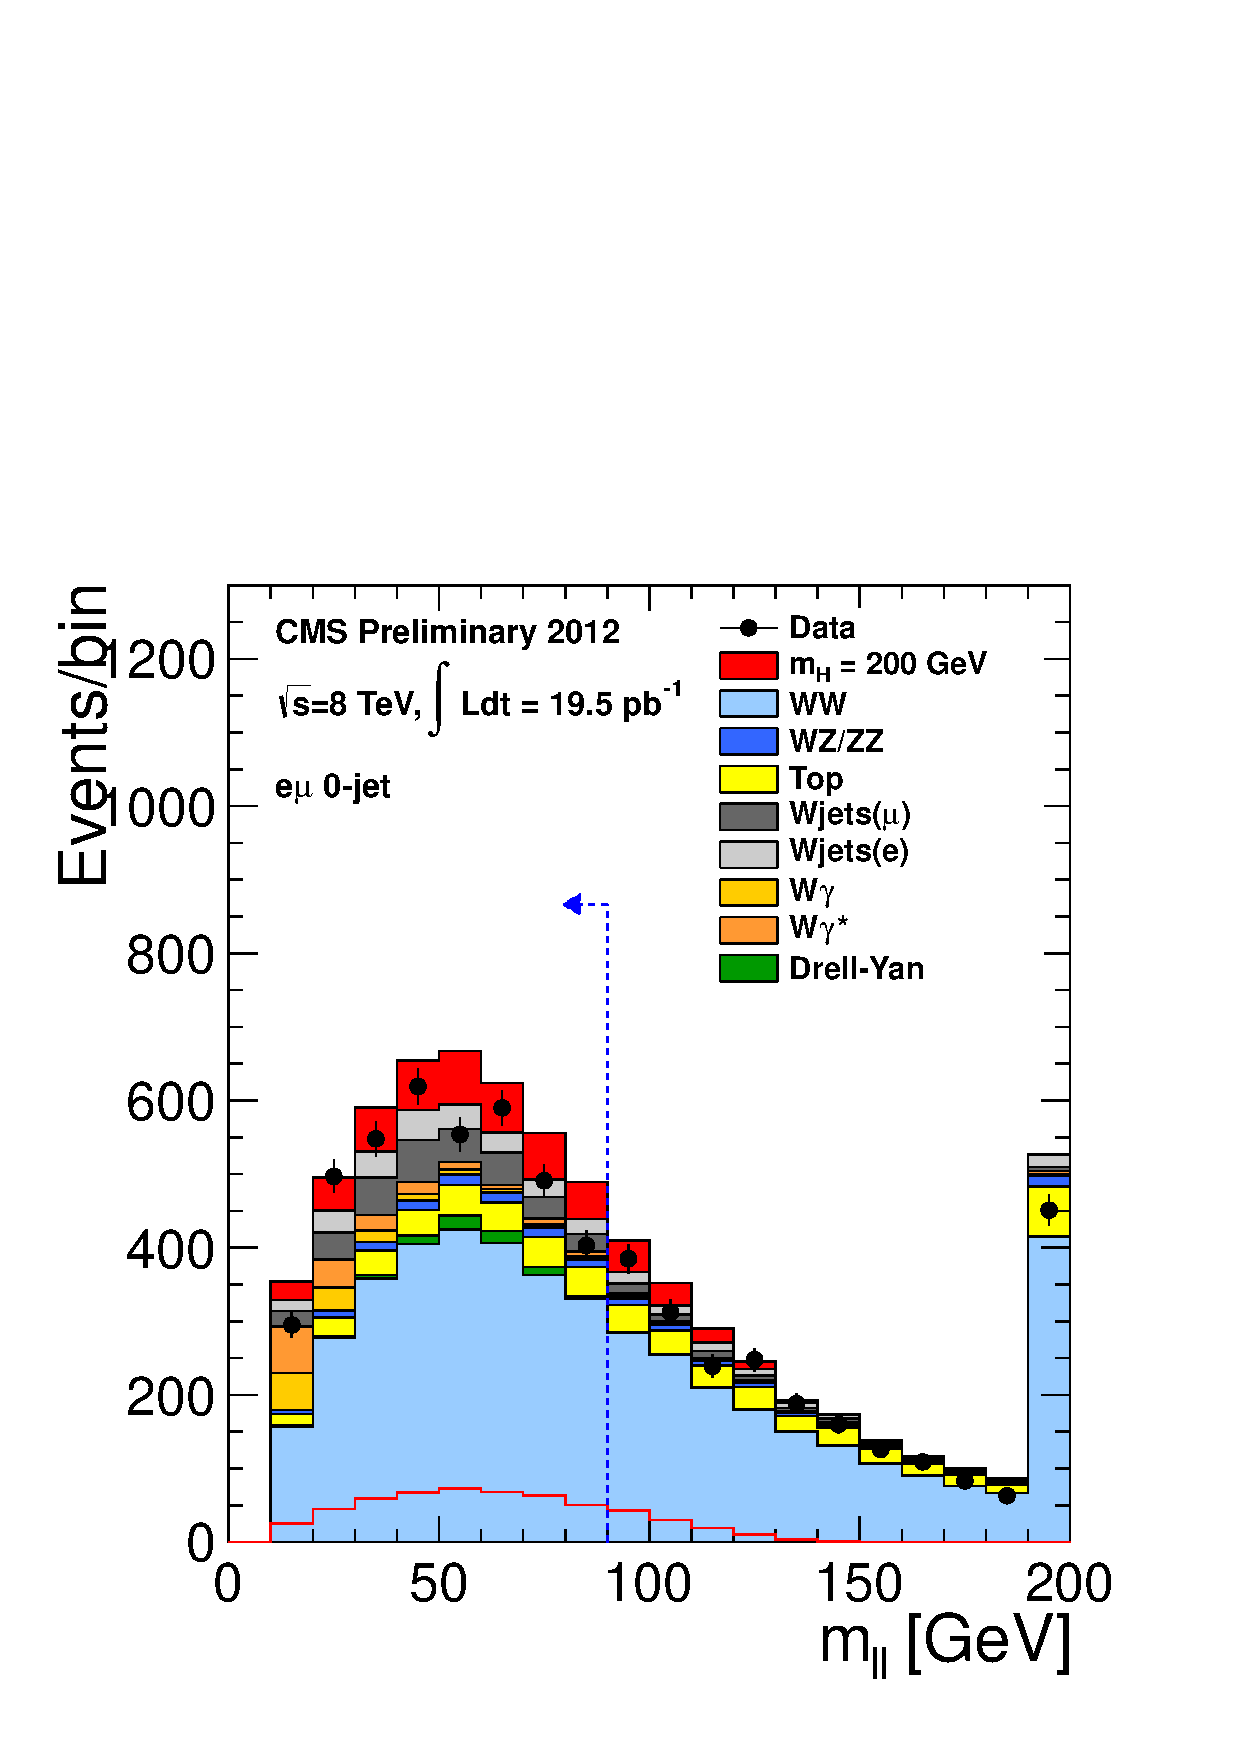
\includegraphics[width=0.45\textwidth]{figures/hww_analysis16_200_ALL_of_0j_mll.pdf}
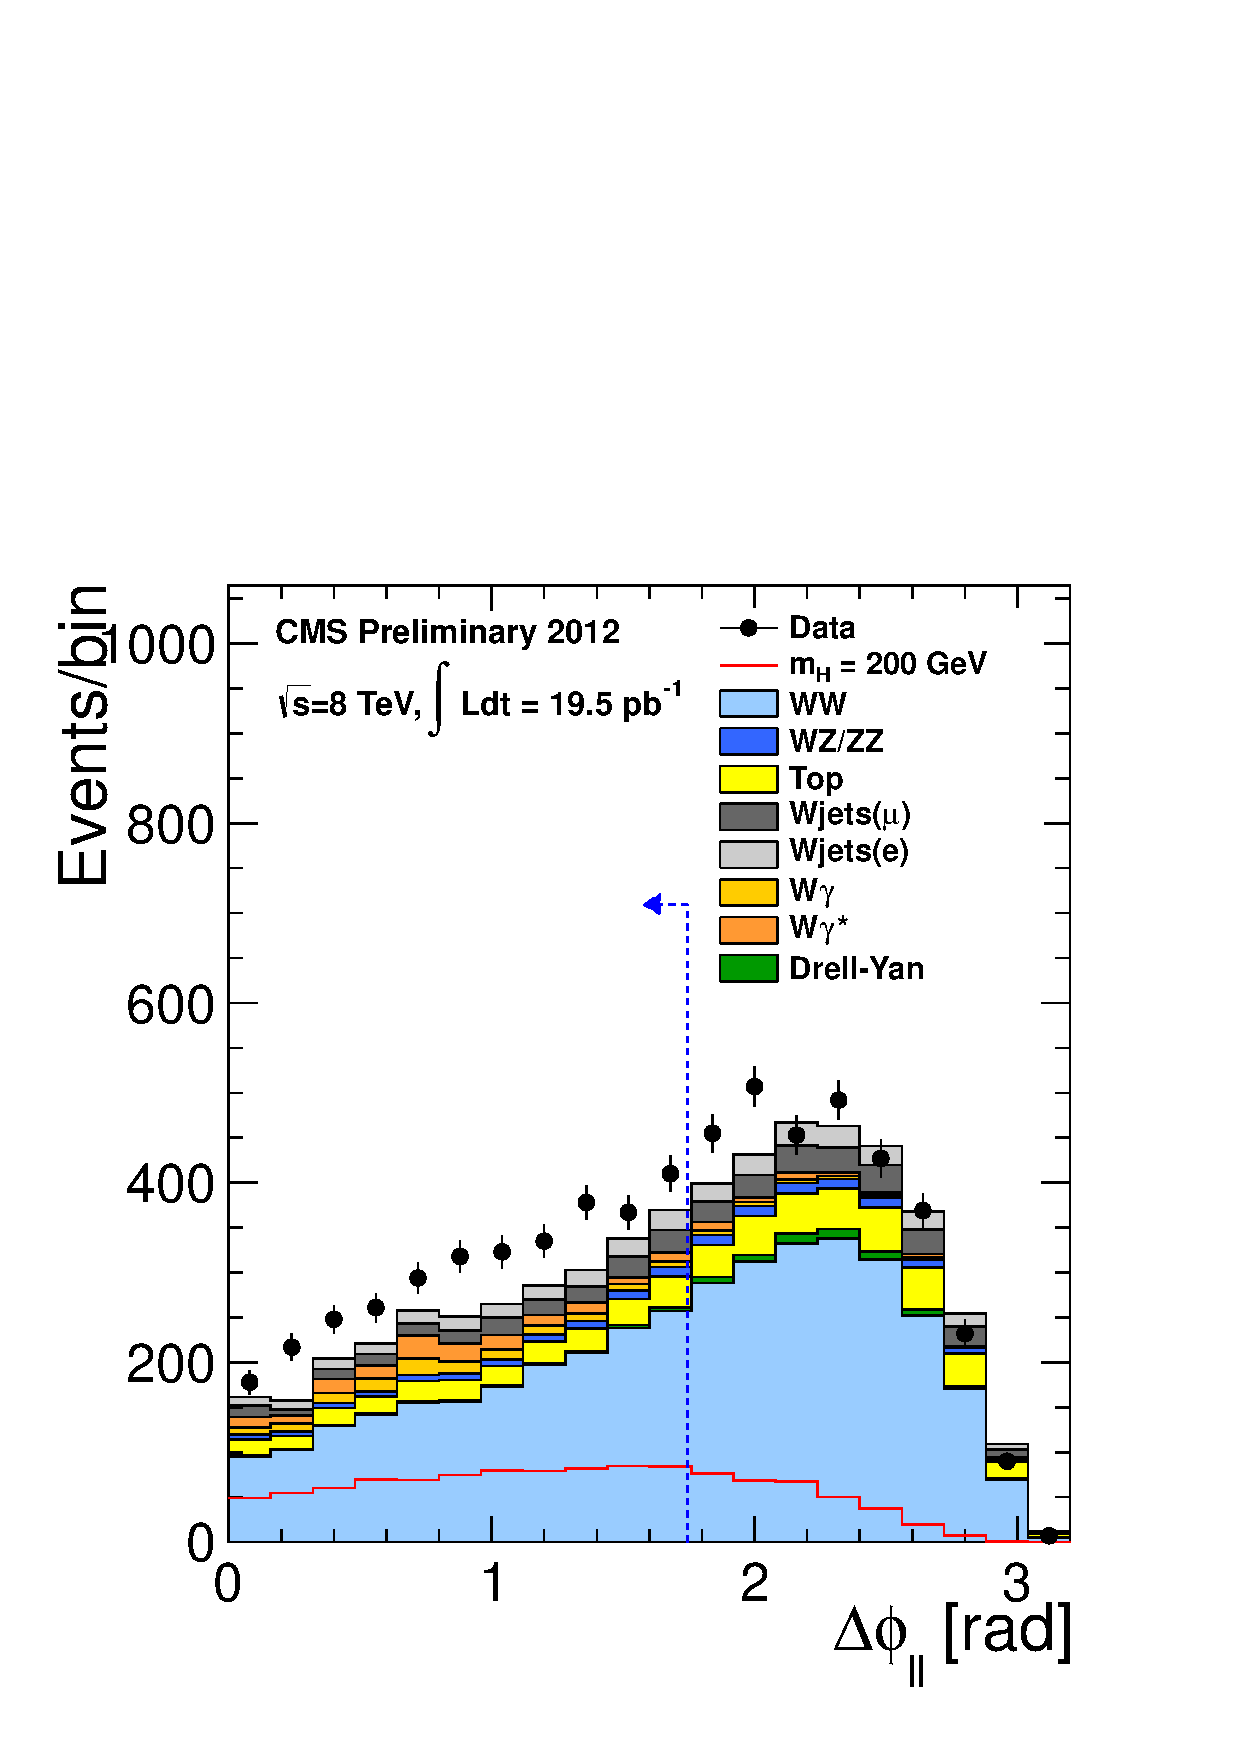
\includegraphics[width=0.45\textwidth]{figures/hww_analysis16_200_ALL_of_0j_dphi.pdf}
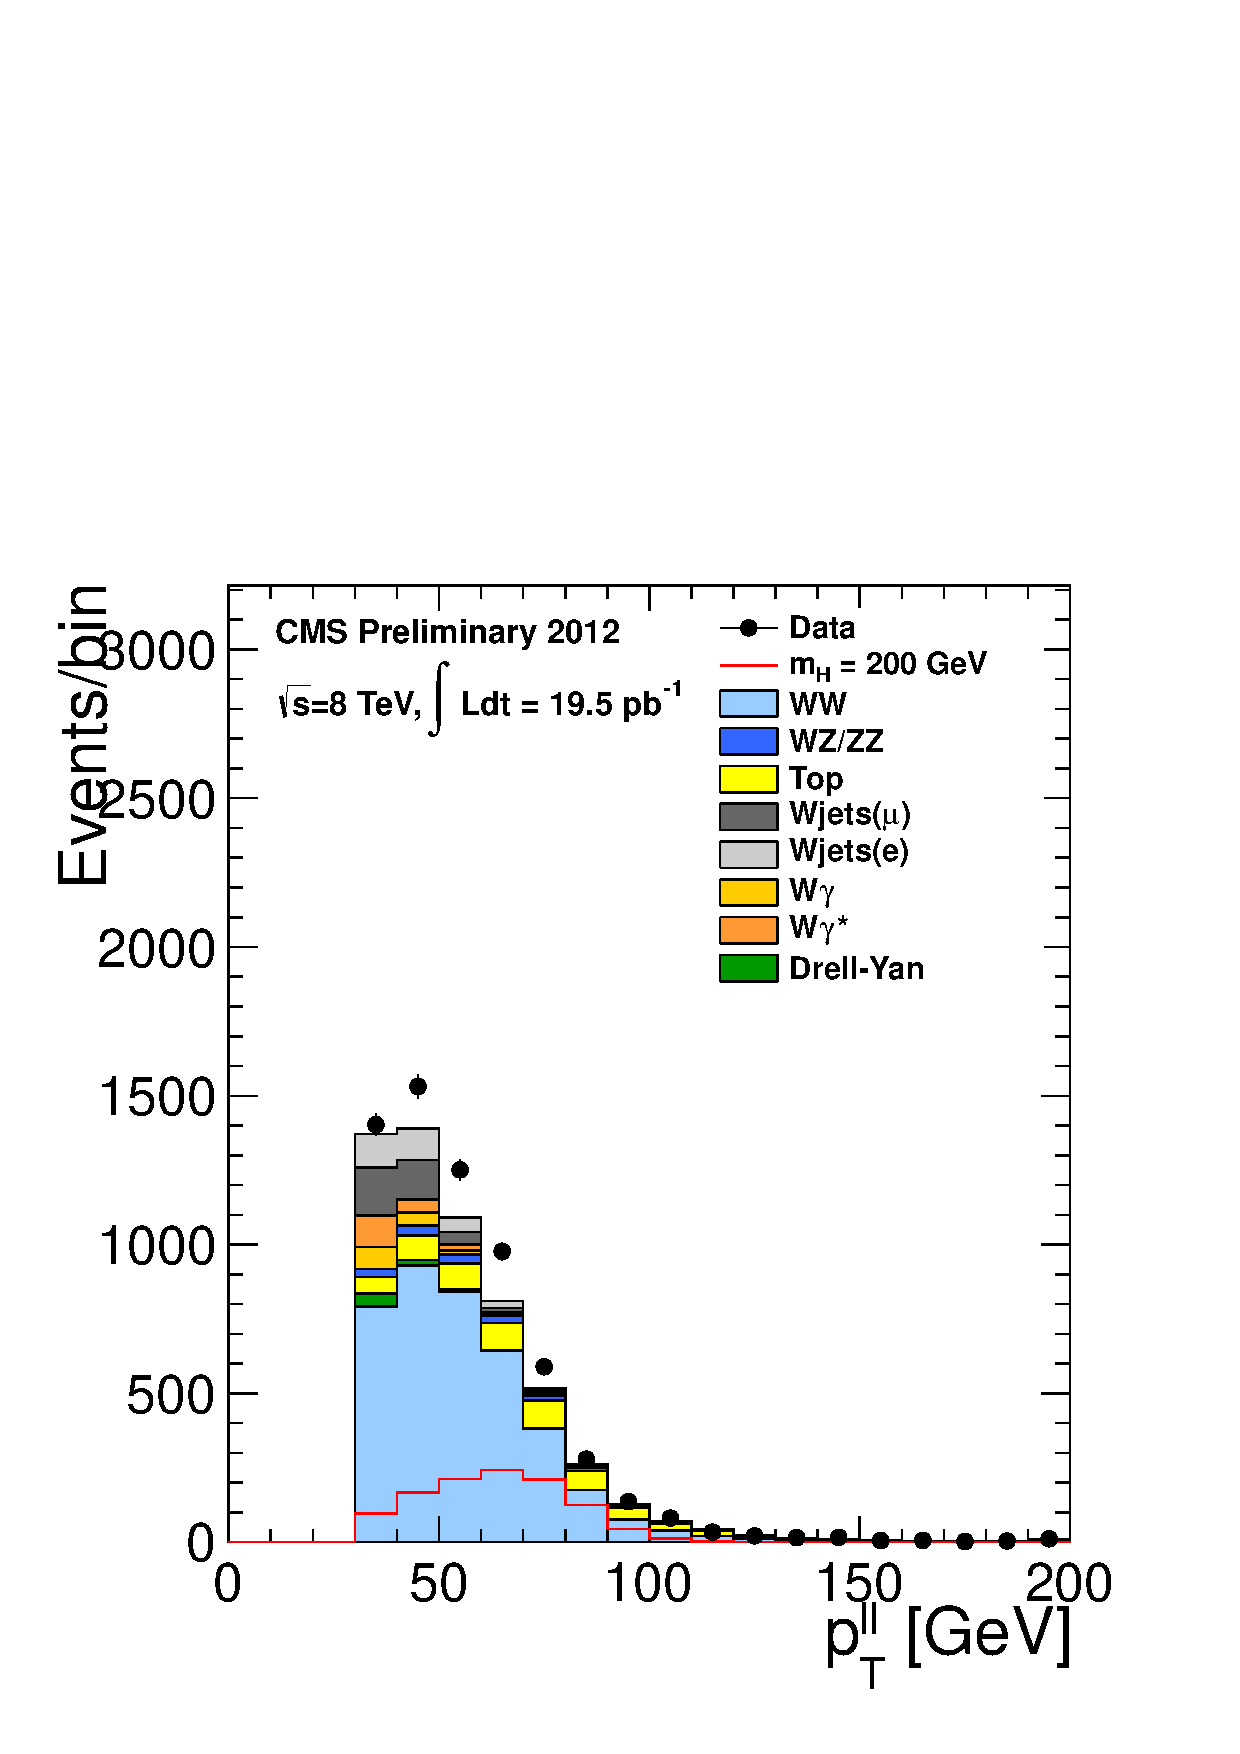
\includegraphics[width=0.45\textwidth]{figures/hww_analysis16_200_ALL_of_0j_ptll.pdf}
\caption{ WW-level plots in 0-jet \DF\ channel with \mHi=200~\GeV\ signal overlaid. 
Cuts for \mHi=200\GeV\ is shown with blue dotted lines and arrows. 
}
\label{fig:wwlevelmh200}
\end{figure}

Figure~\ref{fig:wwlevelmh125}-\ref{fig:wwlevelmh200} show the signal and background distributions of the five variables 
at WW-level for 4 \mHi\ hypotheses at 125, 160 and 200~\GeV. 
The signal is overlaid on the background.  
%
\begin{table}[!ht]
  \begin{center}
 {\small
  \begin{tabular} {|c|c|c|c|c|c|c|}
  \hline
\mHi~[\GeV] & \ptlmax~[\GeV] & \ptlmin~[\GeV] & \mll~[\GeV]   & \delphill~[$\cdot$] 
            & \mT~[\GeV] \\  
  \hline 
            &   $>$          &   $>$          &   $<$         &  $<$             
            &            \\  
  \hline \hline
    115 & 20  &  10     & 40  & 115 & 80 - 110  \\
    120 & 20  &  10     & 40  & 115 & 80 - 120  \\
    125 & 23  &  10     & 43  & 100 & 80 - 123  \\
    130 & 25  &  10     & 45  & 90  & 80 - 125  \\
    135 & 25  &  12     & 45  & 90  & 80 - 128  \\
    140 & 25  &  15   	& 45  & 90  & 80 - 130  \\
    145 & 25  &  15   	& 45  & 90  & 80 - 130  \\
    150 & 27  &  25   	& 50  & 90  & 80 - 150  \\
    160 & 30  &  25   	& 50  & 60  & 90 - 160  \\
    170 & 34  &  25   	& 50  & 60  & 110 - 170 \\
    180 & 36  &  25   	& 60  & 70  & 120 - 180 \\
    190 & 38  &  25   	& 80  & 90  & 120 - 190 \\
    200 & 40  &  25   	& 90  & 100 & 120 - 200 \\
    250 & 55  &  25   	& 150 & 140 & 120 - 250 \\
    300 & 70  &  25   	& 200 & 175 & 120 - 300 \\
    350 & 80  &  25   	& 250 & 175 & 120 - 350 \\
    400 & 90  &  25   	& 300 & 175 & 120 - 400 \\
    450 & 110 &  25   	& 350 & 175 & 120 - 450 \\
    500 & 120 &  25   	& 400 & 175 & 120 - 500 \\
    550 & 130 &  25   	& 450 & 175 & 120 - 550 \\
    600 & 140 &  25   	& 500 & 175 & 120 - 600 \\
  \hline
  \end{tabular}
  }
  \caption{\mHi-dependent event selection for the cut-based analysis 
           in the 0-jet and 1-jet categories. }
   \label{tab:cutbasedtable}
  \end{center}
\end{table}

Table~\ref{tab:cutbasedtable} shows the cut values depending on the \mHi. 
Applying these cuts improve S/B from XX to YY. 






%%%%%%%%%%%%%%%%%%%%%%%%%%%%%%%%%%%%%%%
\section{Shape-based Method}
\label{sec:shape}
\begin{itemize} 
\item Motivation : easier interpretation, simpler implementation  
\item applied to only $e\mu$ channel due to poor modeling of DY shape in $ee/\mu\mu$   
\item Choice of variables : mass-like ones
\item Binning: avoid poor stat, empty bins in bkgd templates. 
      show relative statistics uncertainty of each bkgd. 
      show S/B with different binning. 
\item Range : show expected significance expanding range from signal region to the full 
      [\mT, \mll] range $\rightarrow$ these are basically what's already in the 2D note 
\item mention that there are two templates for low/high \mHi. 
      additional selection($\ptlmax>50\GeV$) for high \mHi~templates
\item now show 2D templates for selective \mHi~points(125,160,200,400) and each background process
      (Show 8TeV 0jet only. The rest will be in the appendix)
\item Technicality : unrolling  procedure. show some unrolled templates and mention that 
      these are what's actually used by Stat machineries. mention correlation is still there. 
\end{itemize}  

The other method, which is called ``2D method" hereafter, 
is shape-based analysis which uses binned 2-dimentional shapes 
of \mT\ and \mll. This method is more complicated than the cut-based method
because it uses the shape and the additional uncertainties to the shape 
on top of normalization should be taken into account. 
To extract the signal component, the 2-dimensional binned shape is fitted to data. 
The shapes for the most of the background are taken from simulation except for 
the \Wjets\ which is taken from data subtacted by simulation. 
Therefore, it is critial to make sure that the fit model correclty describes 
what is observed in data. There was a hugh effort to validate this using 
pseudo-data and data-control region. Chapter~\ref{ch:fit_validation} describes 
the details. 

There are two main motivations for developing this analysis method. 
Before this method was employed as the main anaylysis method for the 
public result of this analysis at CMS, BDT-based multivariate method 
had been the main method \cite{CMS-PAS-HIG-12-038}. Because of 
the non-trivial dependence of the discriminator value(BDT output)
on the input variables, it was very difficult to have 
physical interpretation of the observed result with this method. 
For example, if there is a fluctuation in data, we do not know where this comes from, 
\textit{i.e.} which input variable is reponsible for this non-expected 
behavior. In addtion, because a single template definition is used, 
it avoids unnecessary statistical fluctuations between the data selected 
for nearby hypotheses.
on the practical side, the implementation of the 
analysis became much simpler compared to the BDT method because of using 
the same background template across different \mHi\ hypotheses
while the BDT method used \mHi-dependent selection as the cut-based 
method. This not only simlified workflow but also allowed to draw some 
interesting plots such as 2-dimensional log likelihood scan in the plane of 
signal strength and \mHi, which were not possible with \mHi-dependent 
selections for technical reasons. 

The modeling of \dyll\ simulation background is quite poor in tail of high \met\
and the statistics of the available MC sample is limited resulting a huge weight. 
Therefore, we can not trust the shape of \dyll\ from simulation and  
the 2D method is applied to \DF\ channels. 

The choice of the variables is motivated by the fact that the best 
variable that discriminates signal from background is the Higgs mass. 
But, due to the neutrinos in the final state, Higgs mass can not be 
reconstructed. Therefore, we use the two \mHi-like variables, 
the higgs transverse mass, \mT,  and the di-lepton mass, \mll\
to construct the 2-dimensional templates. These two variables are 
weakly correlated in the main background processes,
\textcolor{red}{why strong correlation for \wgamma, \wgammastar?} 
allowing maximum advantage of using two variables.  
\textcolor{blue}{show bin-normalized templates for 125/160/250 and qqww 
and mention that signal vs. qqww, signal vs. signal(data should be able to 
distinguish different hypotheses) comparison}
\begin{figure}[htp]
\centering
\subfigure[$\mHi=125~\GeV$]{
\centering
\label{subfig:2dNormBin_mH125}
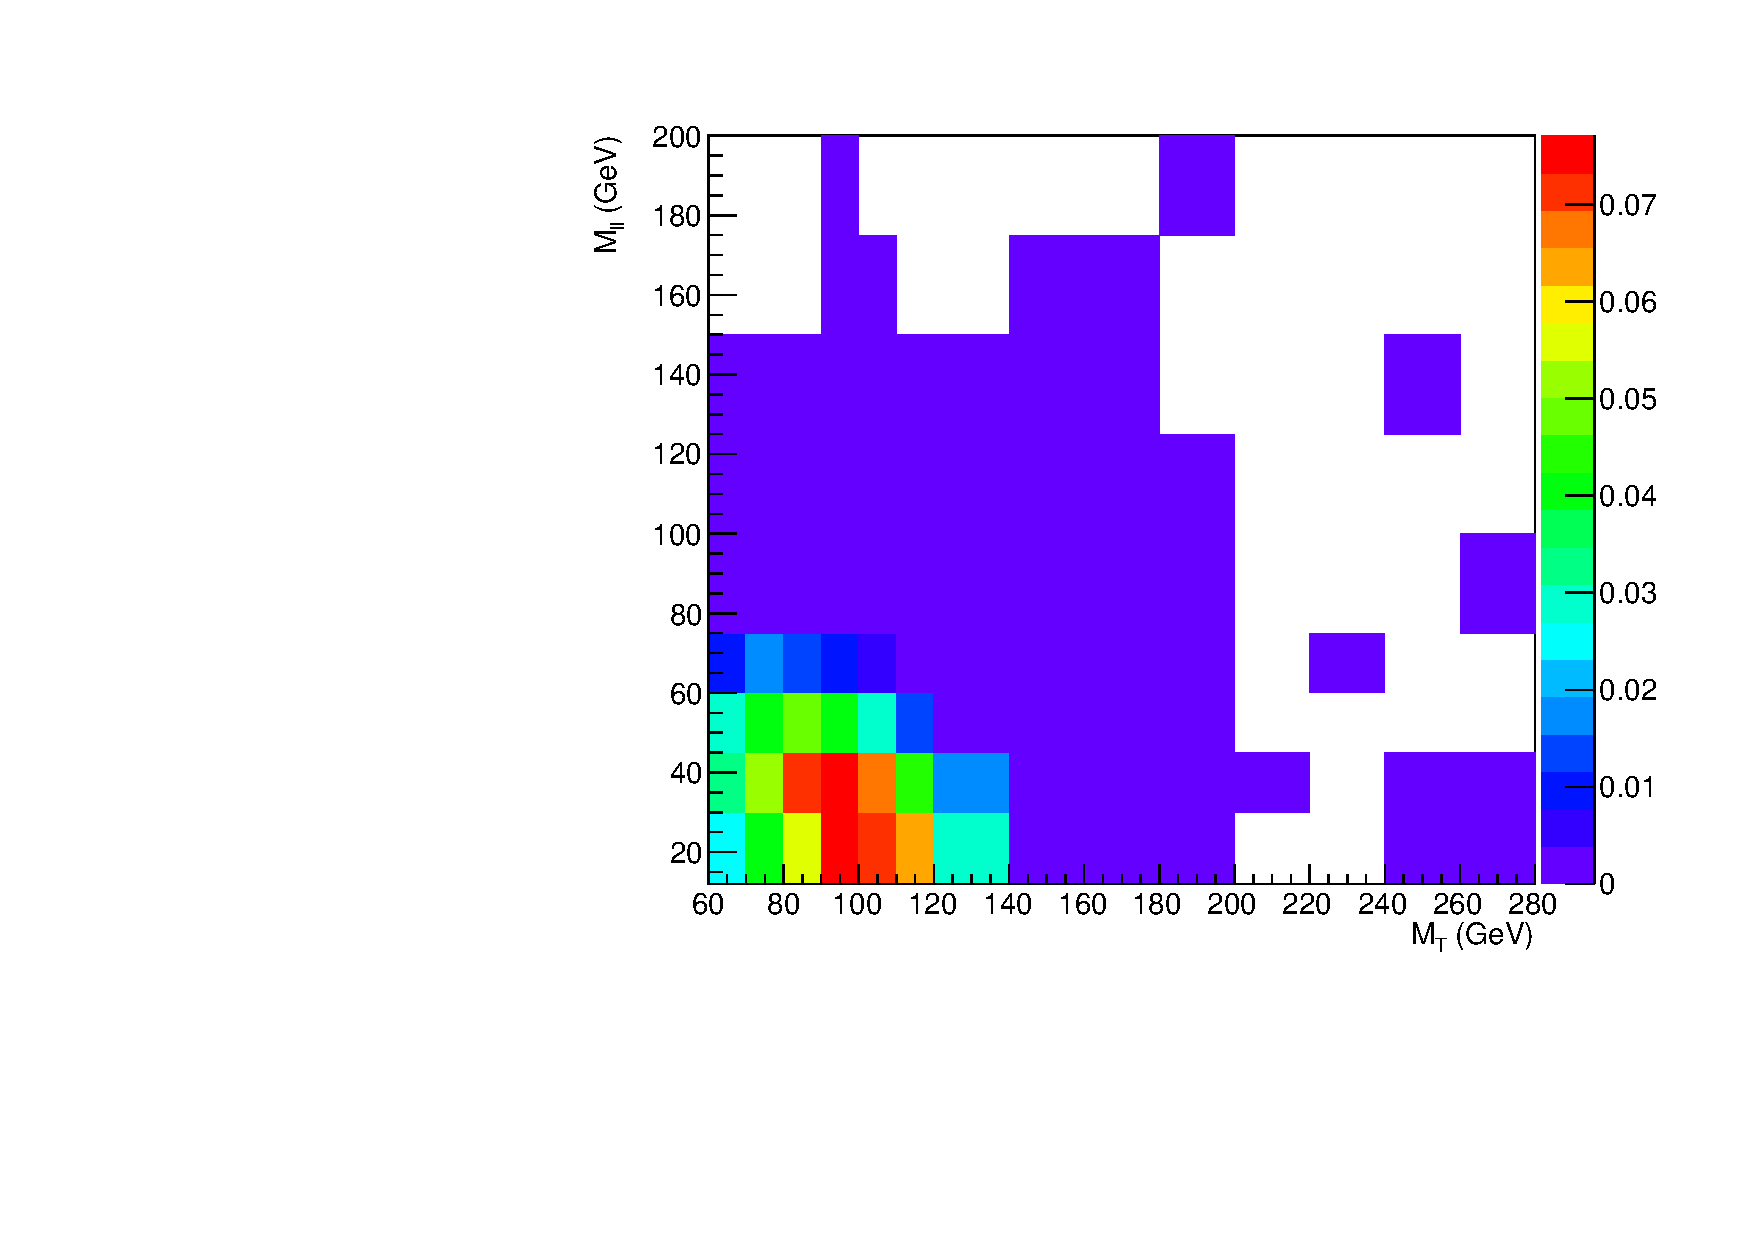
\includegraphics[width=0.45\textwidth]{figures/2dNormBin_mH125.pdf}
}
\subfigure[$\mHi=160~\GeV$]{
\centering
\label{subfig:2dNormBin_mH160}
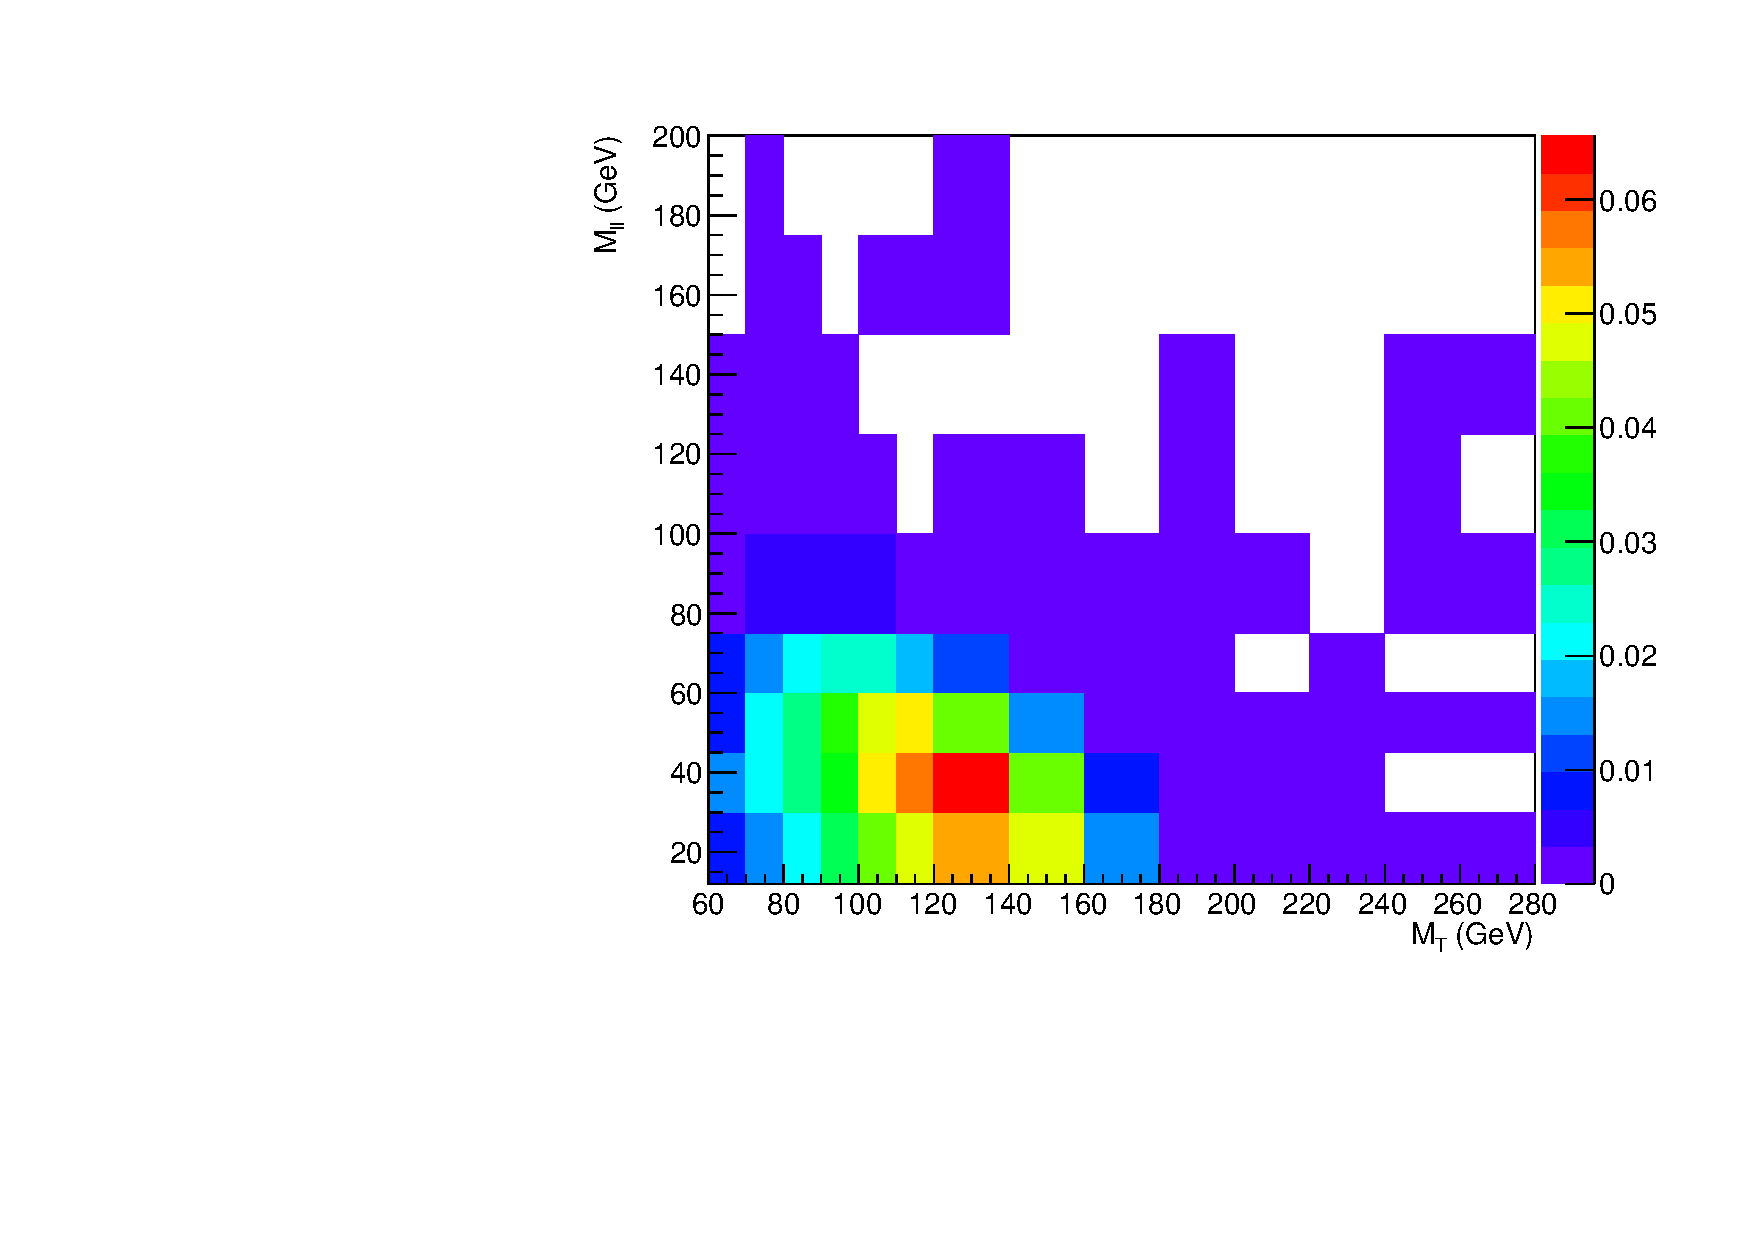
\includegraphics[width=0.45\textwidth]{figures/2dNormBin_mH160.pdf}
}
\subfigure[$\mHi=200~\GeV$]{
\centering
\label{subfig:2dNormBin_mH200}
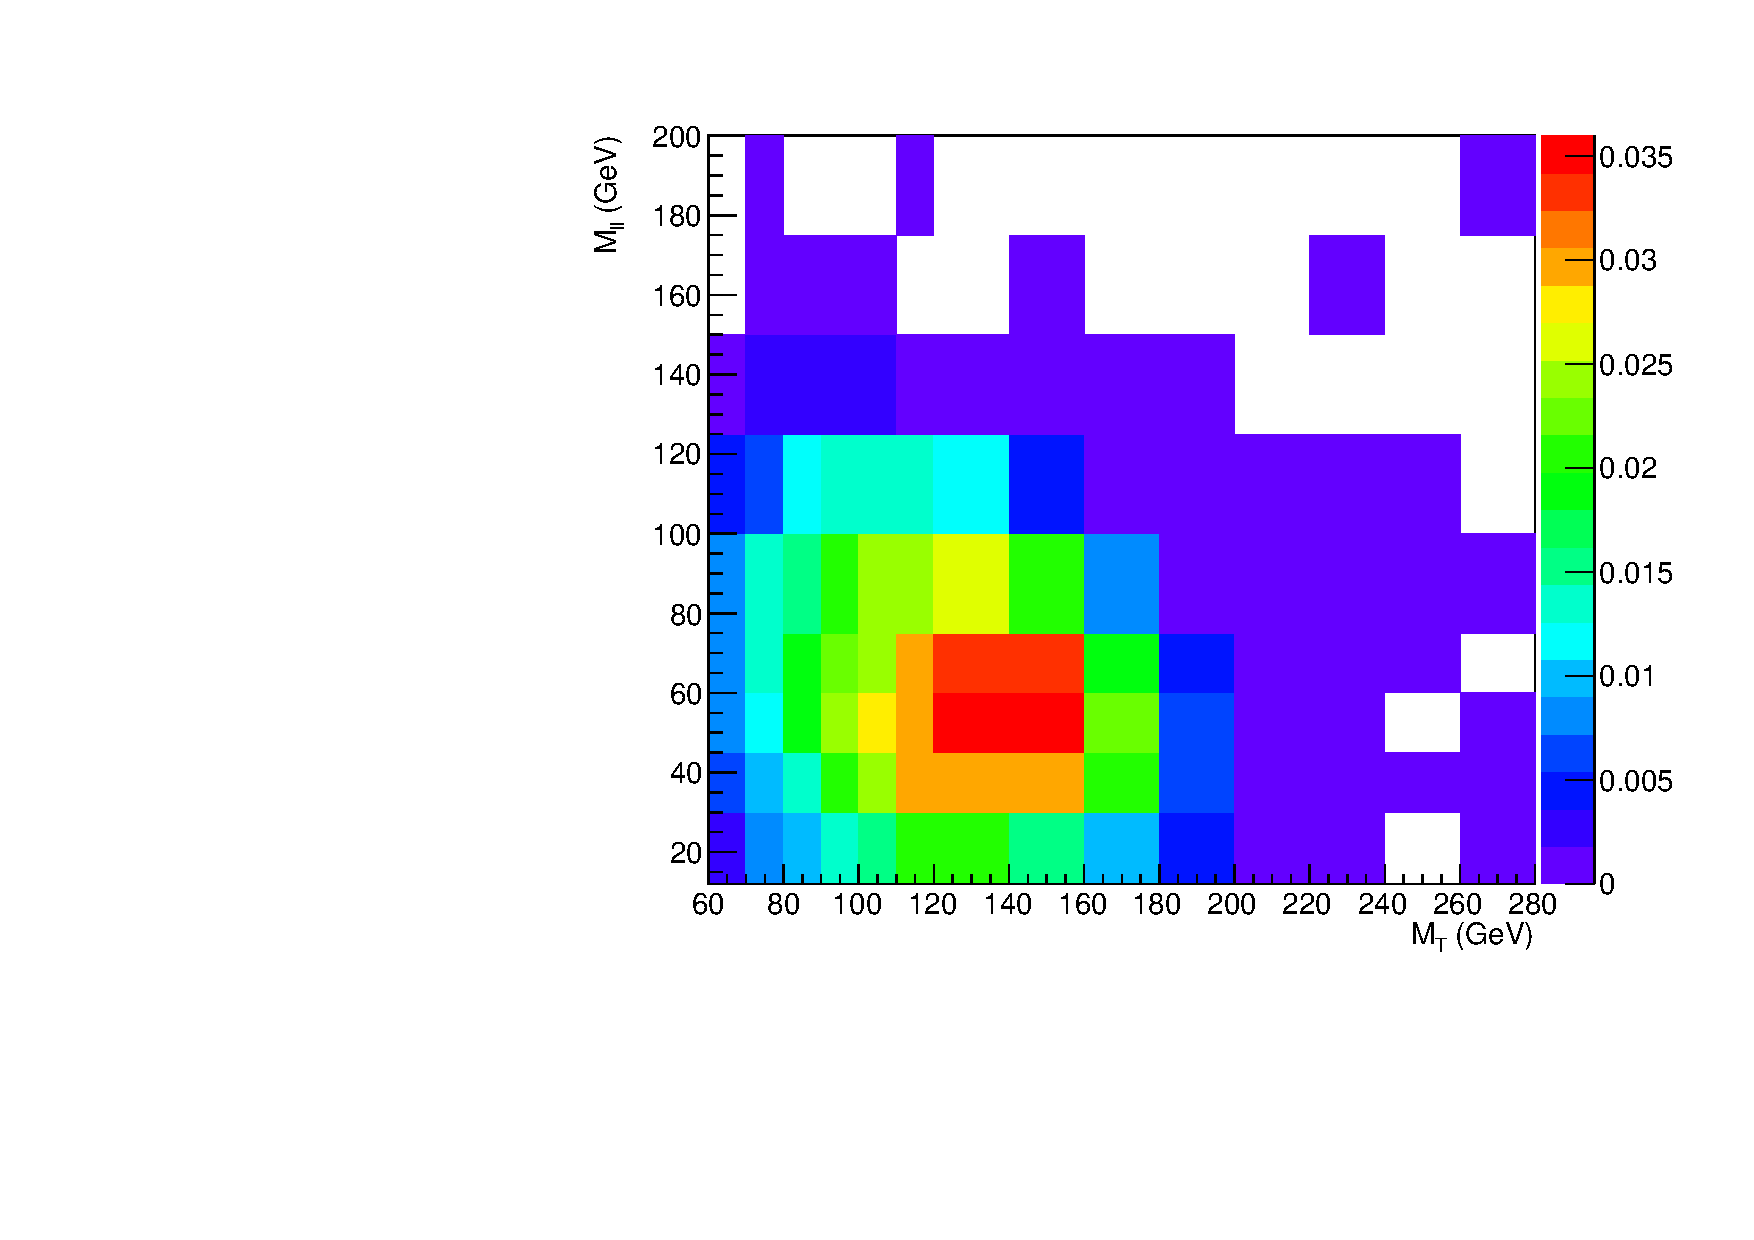
\includegraphics[width=0.45\textwidth]{figures/2dNormBin_mH200.pdf}
}
\subfigure[\qqww]{
\centering
\label{subfig:2dNormBin_qqWW}
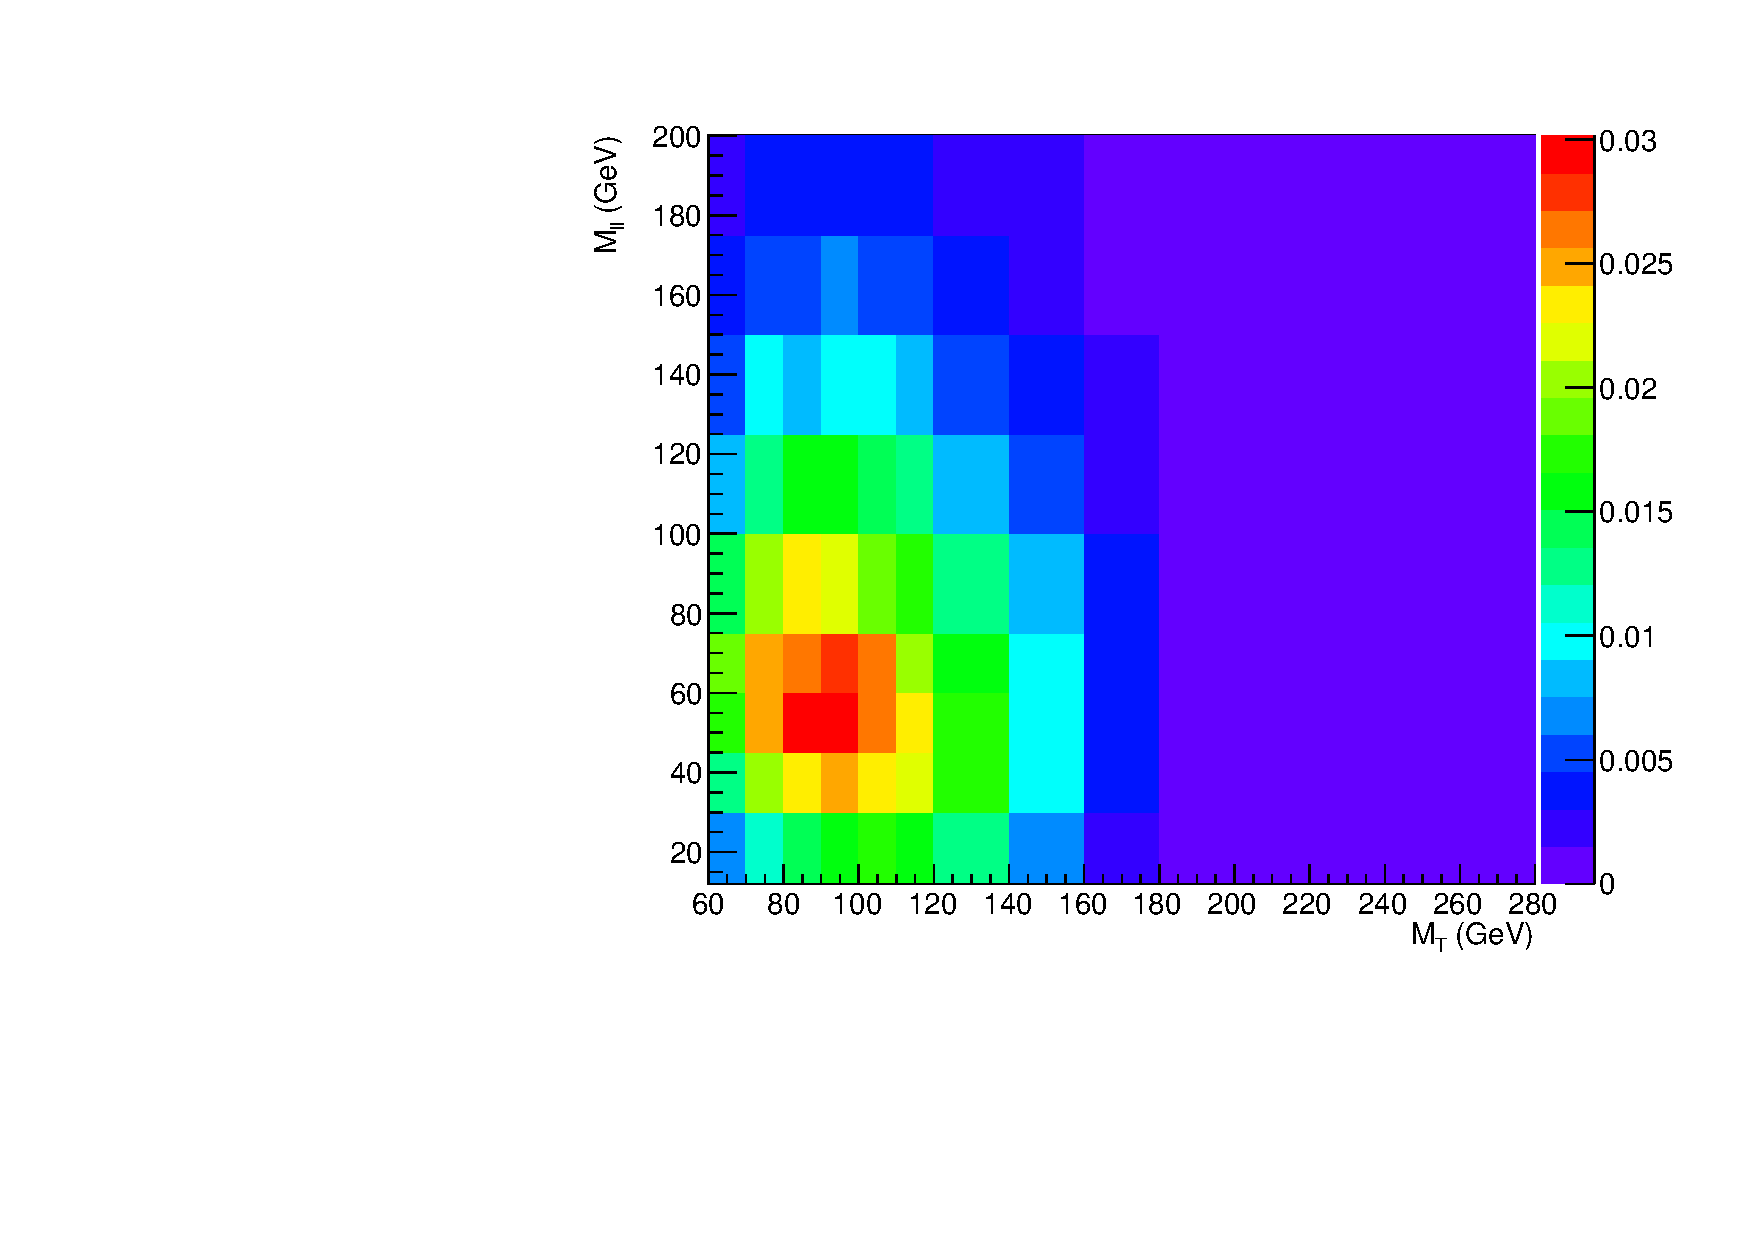
\includegraphics[width=0.45\textwidth]{figures/2dNormBin_qqWW.pdf}
}
\caption{ 2D templates for $\mHi=125, 160, 200~\GeV$ and \qqww. 
For visualization, each bin is divided by 
the area of the bin in order to avoid random peaks due to difference in the bin size.  
}
\label{fig:2dNormBin}
\end{figure}


For the determination of the range and the binning, following points were considered : 
\begin{itemize}
\item Range should cover multiple \mHi\ with one template definition
\item Binning should allow enough granuality to distinguish the signal from the background 
      in the region where signal is populated : sideband region can have coarser binning 
      in case of low statistics in that region
\item statistical uncertainty of the templates should be small with respect to the 
      total background : otherwise the templates will not be reliable  
\item There should not be any empty bin when all backgrounds are summed : otherwise any excess 
      in data will claim infinite significance, \textit{i.e.} something is observed when nothing 
      expected
\item The data events in the bins should be reasonably populated so that the nuisances 
      can be constrained by data
\end{itemize}

Due to large difference in the kinematics of signal events at different \mHi, 
we decided to use two definitions of templates, one for low Higgs mass, 
\mHi = 110 - 250~\GeV, and one for high Higgs mass, \mHi = 300 - 600~\GeV. 
In order to furthur enhance S/B, $\ptlmax>50~\GeV$ is applied for the 
high \mHi\ templates. 
So, for the low(high) \mHi\ hypotheses, we use 
$60 < \mT < 280~\GeV$($60 < \mT < 380~\GeV$)
and 
$0 < \mll < 280~\GeV$($0 < \mll < 450~\GeV$).
The events with high \mHi\ hypothesis tend to have high \mT\ and high \mll\, 
but this is the phase space where background processes are not populated. 
Thus, for the high \mHi\ templates, the top and the right bins are overflow bins 
allowing events up to $\mll<600~\GeV$ and $\mT<600~\GeV$, 
which covers \mHi\ hypothesis up to 600~\GeV.

The resolution of \mT\ and \mll\ is 20 - 25 \GeV\ for low \mHi\ events\footnote{At WW level, \mT\ resolution in the 0-jet(1-jet) category is 20(25)~\GeV\ 
for \mHi = 125~\GeV. The \mll\ resolution is 20~\GeV\ in both 0-jet(1-jet) category.}, 
we take 20-25~\GeV as the maximum size of the a bin for low \mHi\ templates.   
\begin{figure}[htp]
\centering
\subfigure[]{
\centering
\label{subfig:SoverB_2d_20_25}
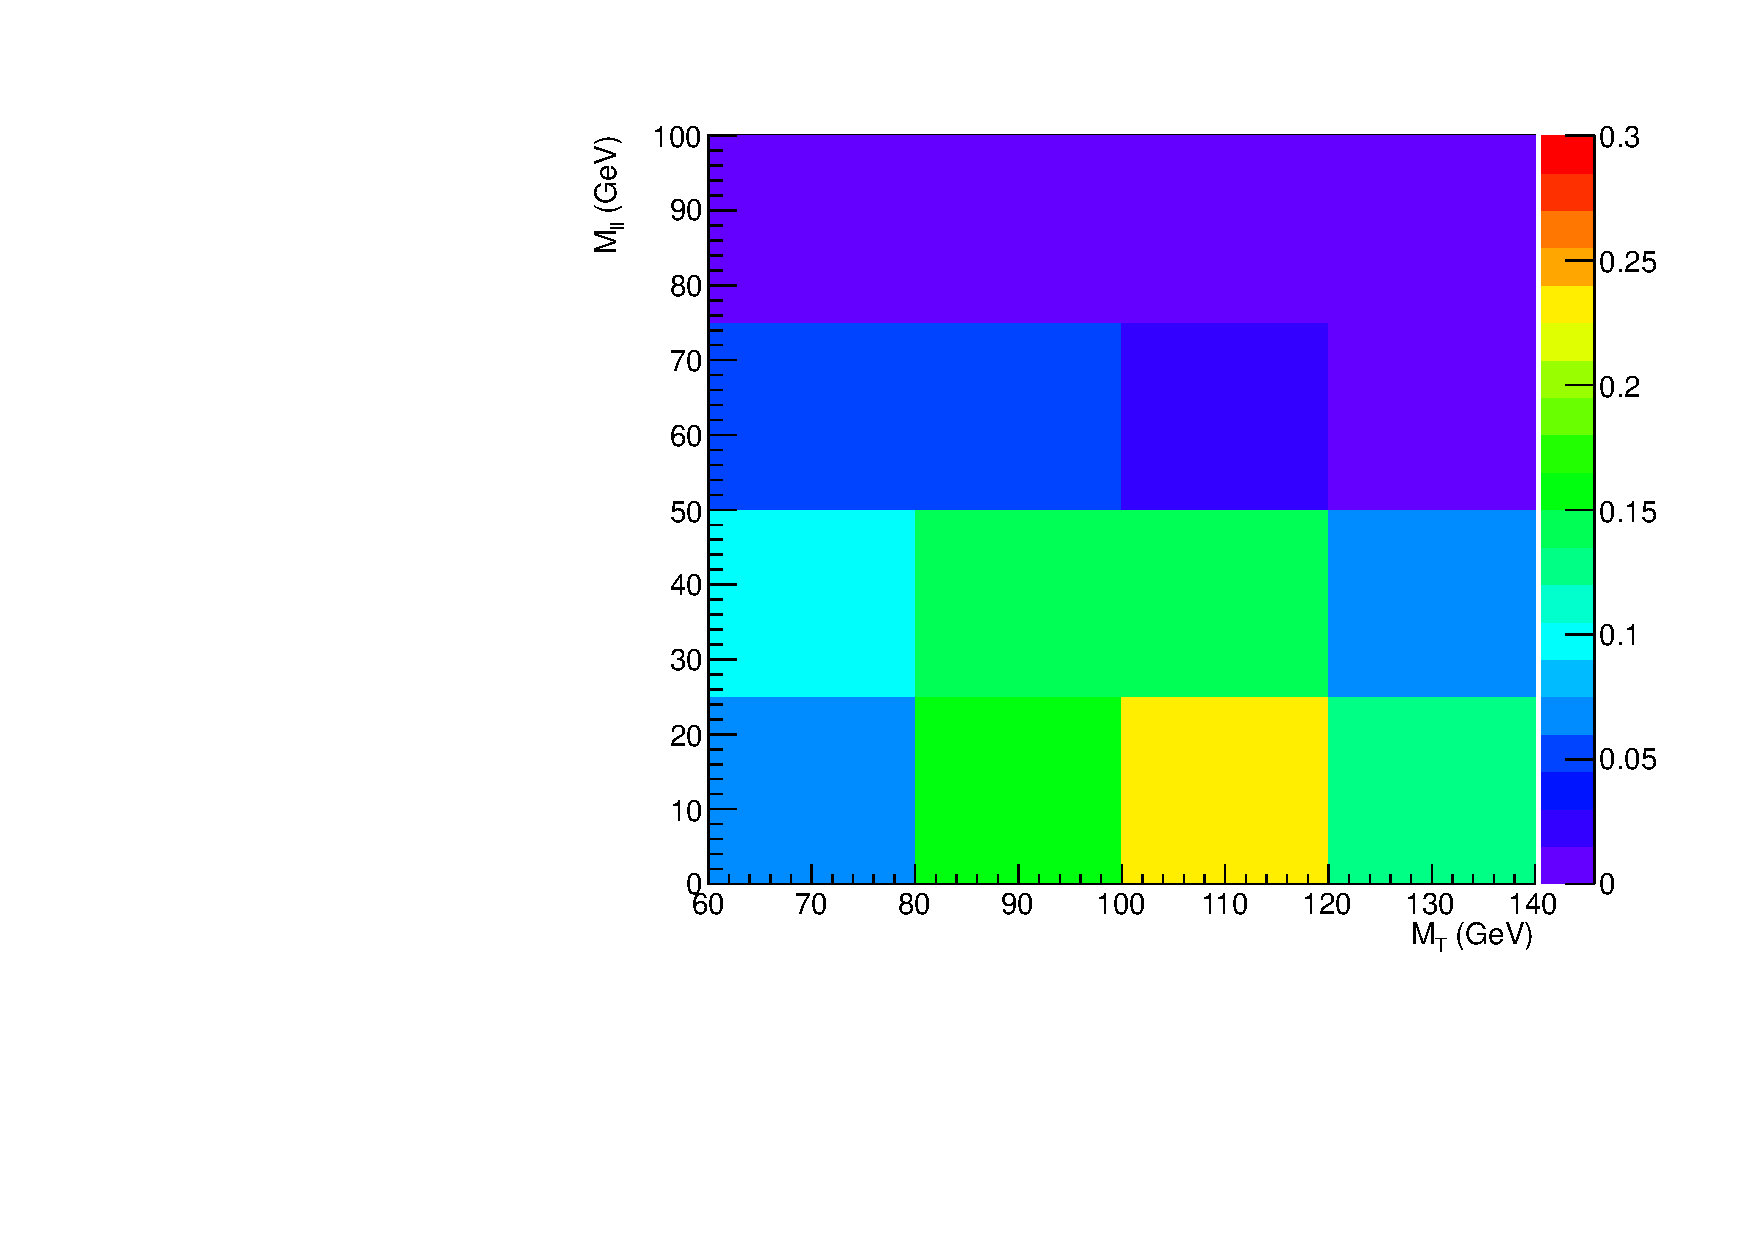
\includegraphics[width=0.45\textwidth]{figures/SoverB_2d_20_25.pdf}
}
\subfigure[]{
\centering
\label{subfig:SoverB_2d_20_10}
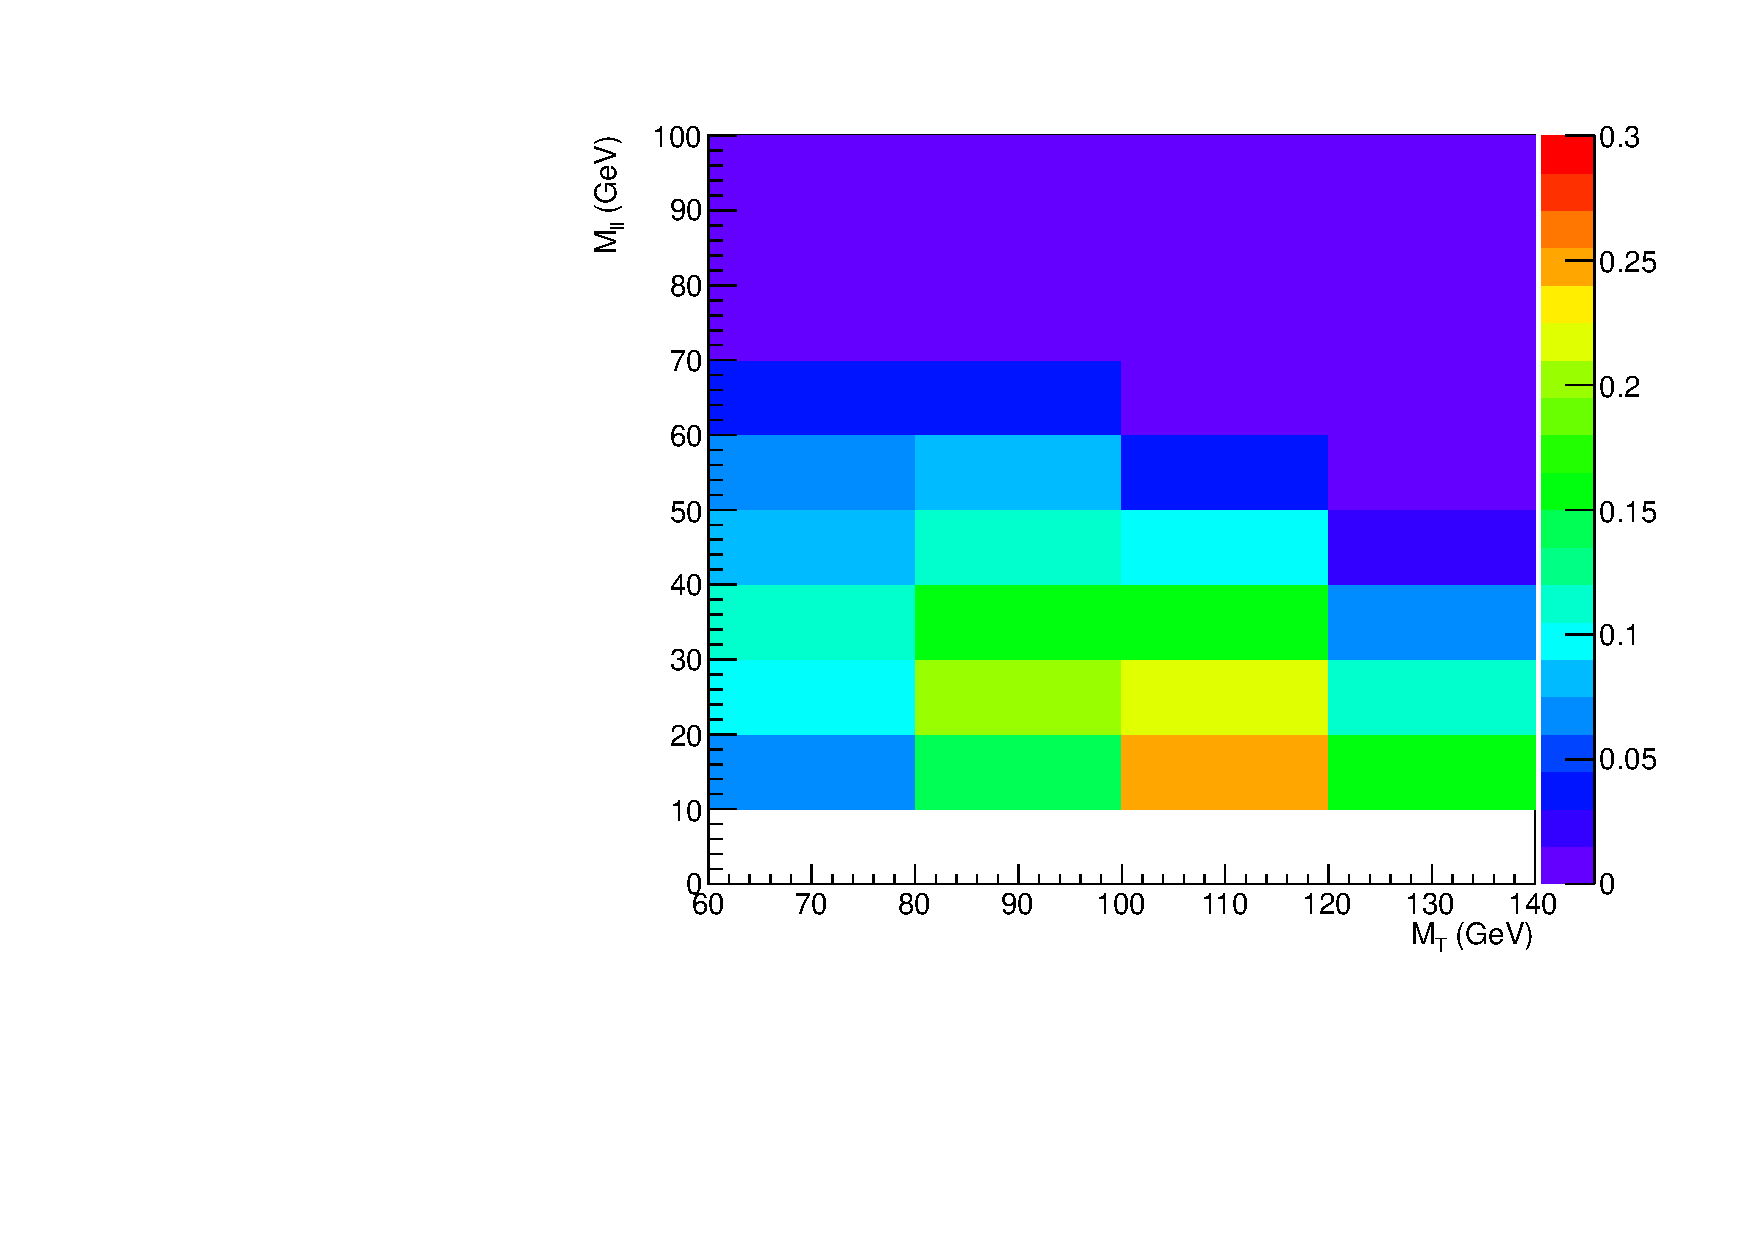
\includegraphics[width=0.45\textwidth]{figures/SoverB_2d_20_10.pdf}
}
\subfigure[]{
\centering
\label{subfig:SoverB_2d_10_25}
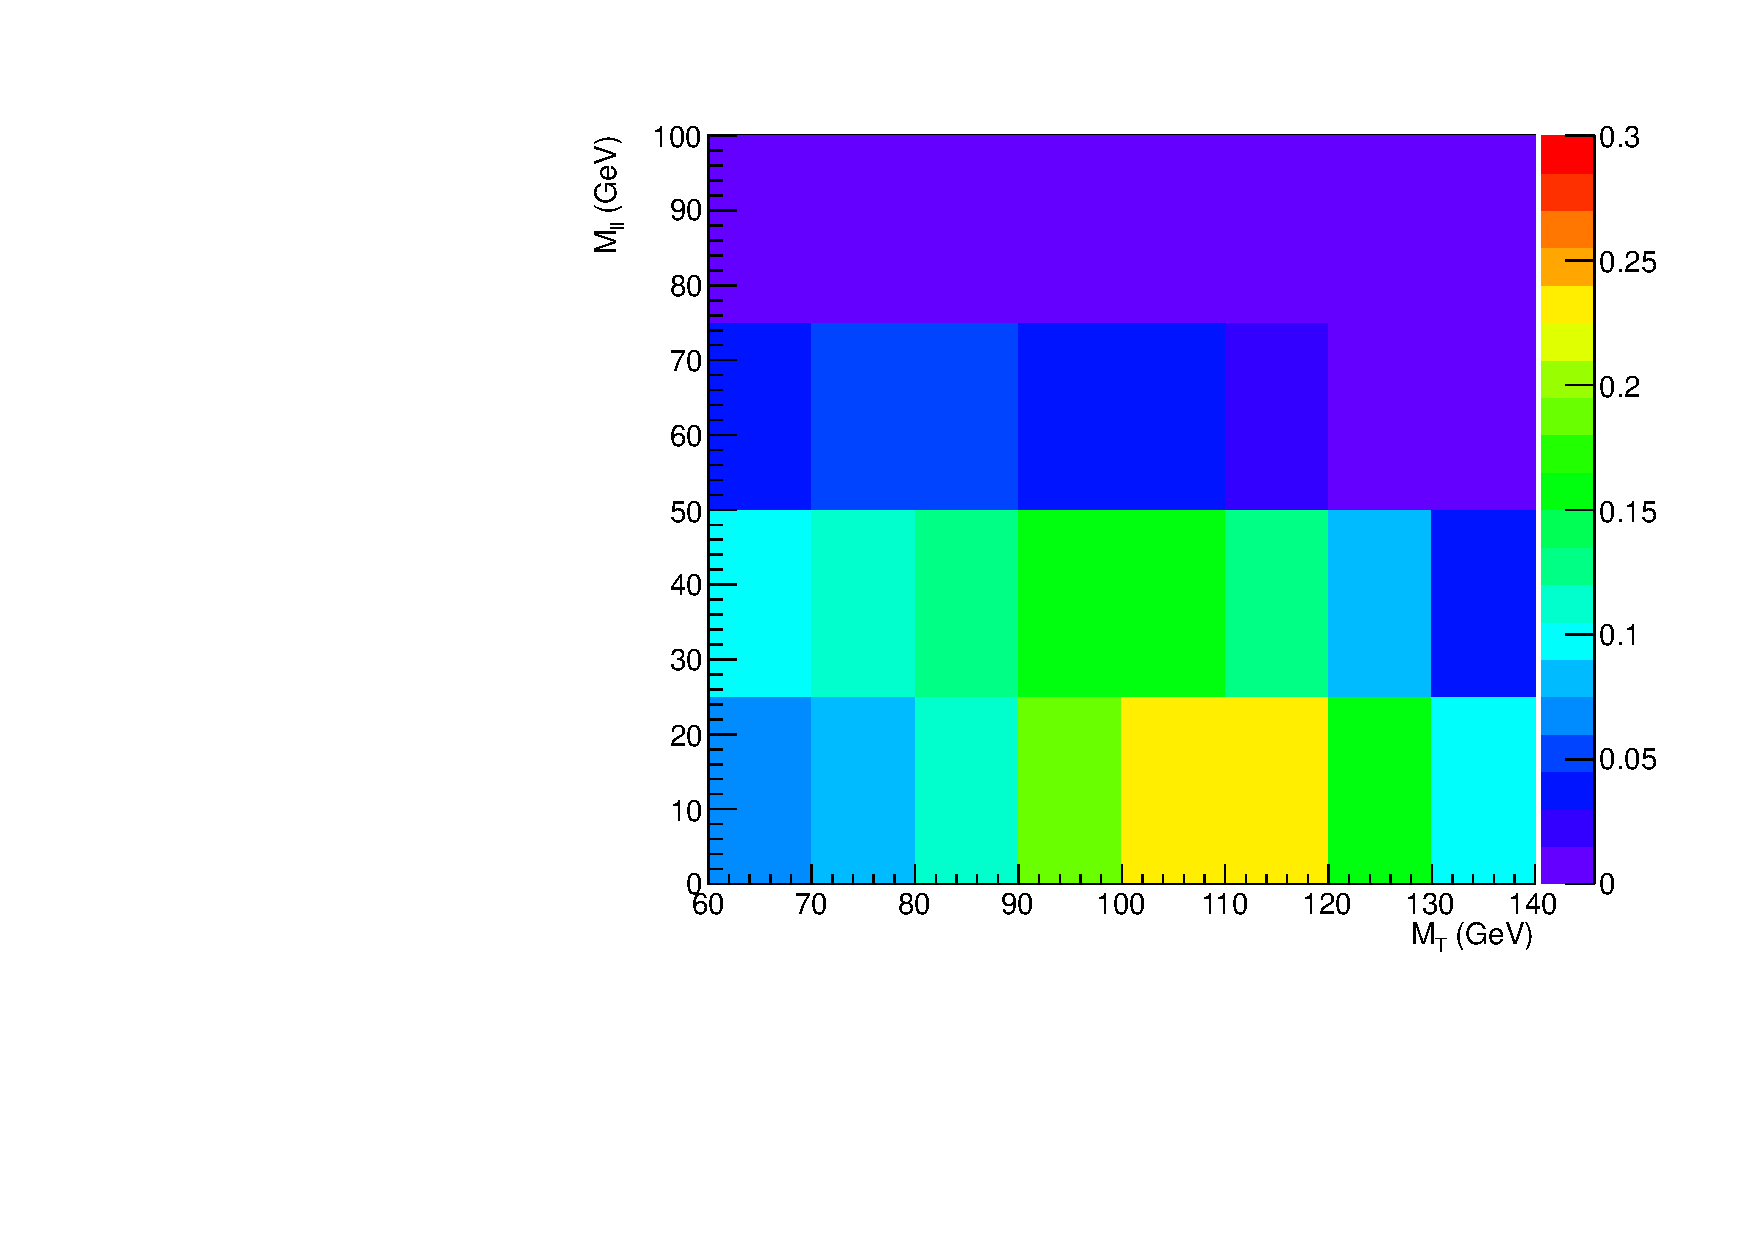
\includegraphics[width=0.45\textwidth]{figures/SoverB_2d_10_25.pdf}
}
\subfigure[]{
\centering
\label{subfig:SoverB_2d_10_10}
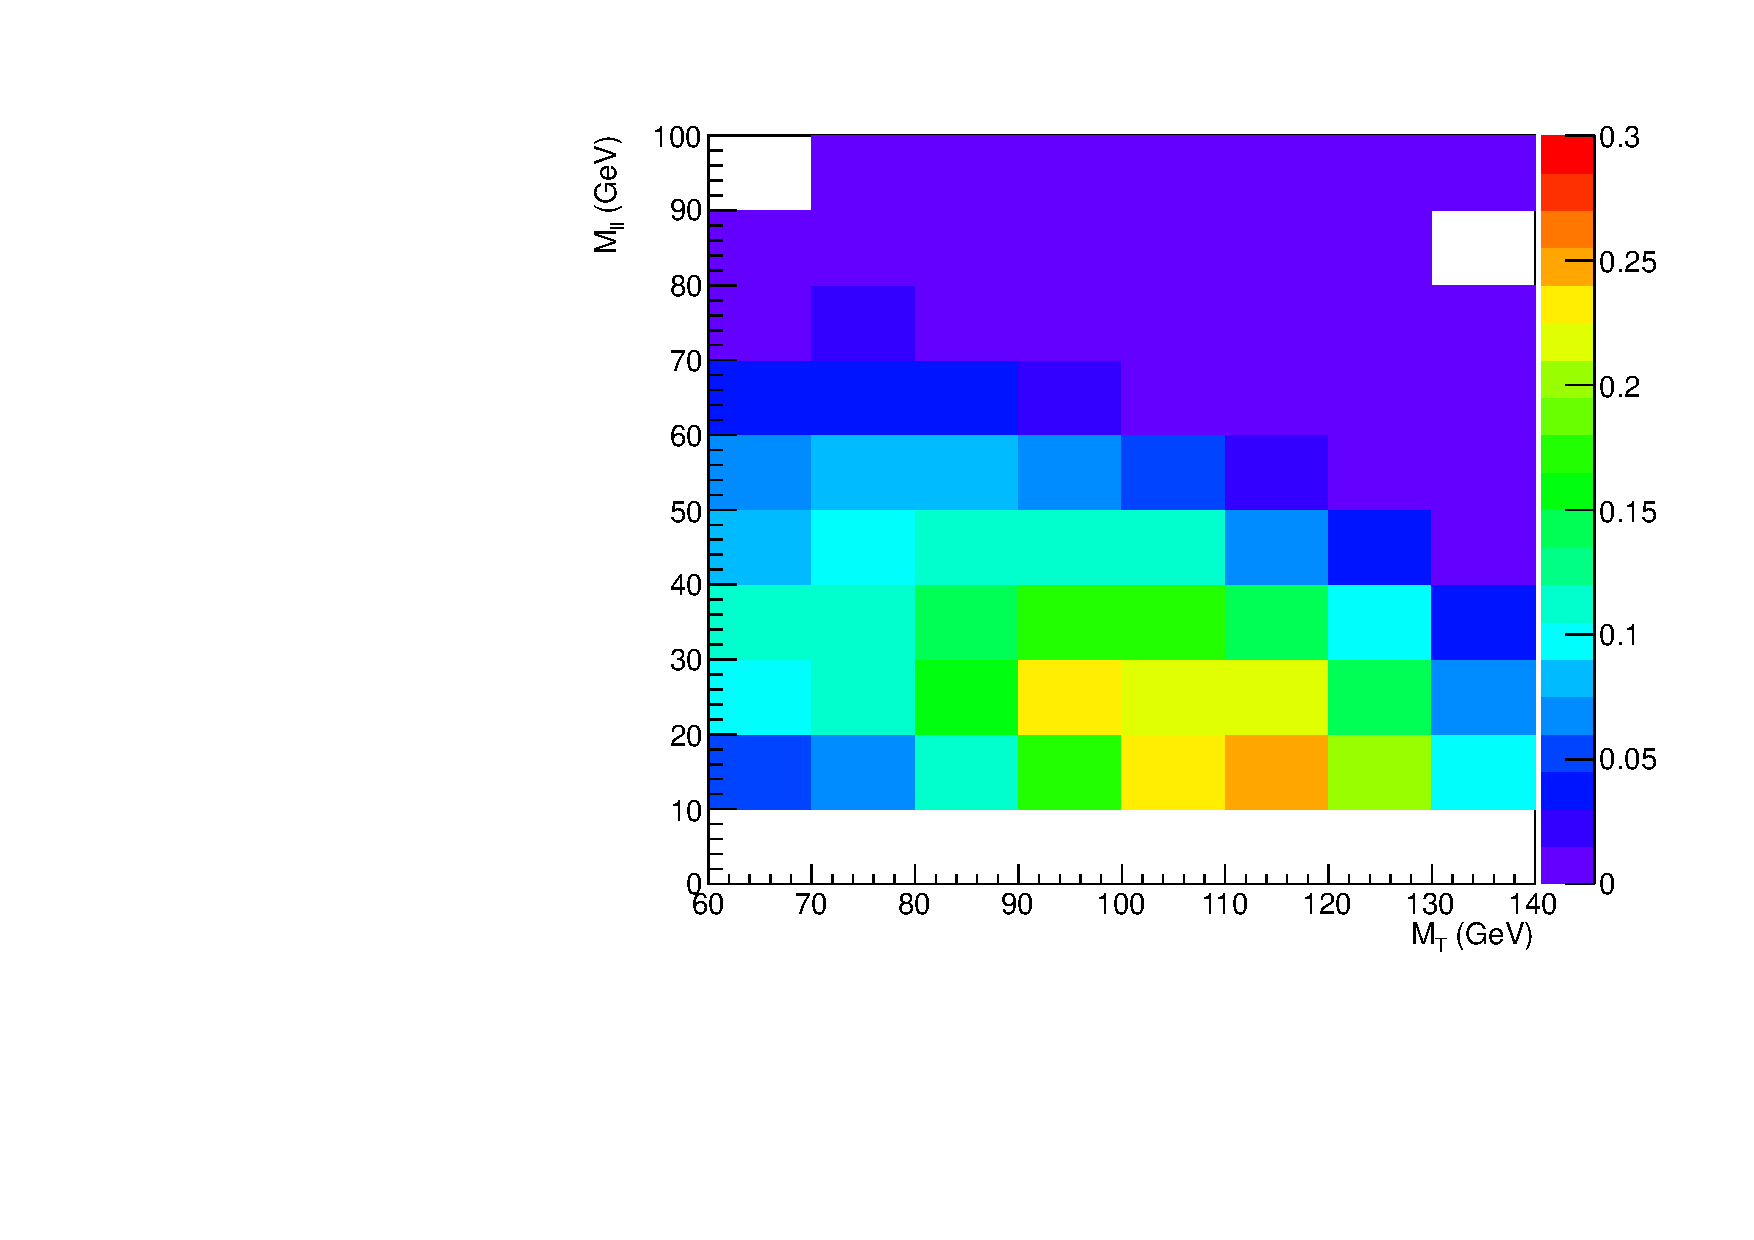
\includegraphics[width=0.45\textwidth]{figures/SoverB_2d_10_10.pdf}
}
\caption{ S/B using different binnings. (a) (b) (c) (d). 
Signal region($60<\mT<120~\GeV$, $0<\mll<100~\GeV$) is zoomed.
}
\label{fig:SoverBdiffbinning}
\end{figure}
Fig.~\ref{fig:SoverBdiffbinning} shows the S/B with 4 different binnings
in the region where \mHi=125~\GeV\ signal is populated($60<\mT<120~\GeV$, $0<\mll<100~\GeV$)
in the 0-jet \DF category ;
bin size of [\mT, \mll]  = [10~\GeV,10~\GeV], [20~\GeV,10~\GeV], 
[20~\GeV,10~\GeV], and [20~\GeV,20~\GeV]. 
The S/B with bin size of 10 - 20~\GeV\ does not change S/B, 
so we can use any bin size in that range. 

\begin{table}[htp] 
\begin{center} 
\vspace{0.5cm}
\begin{tabular}{c|c|c||c|c|c} 
\hline
binning & range & expected & binning & range & expected  \\
$\mT \times \mll$ & [\GeV]  & significance & $\mT \times \mll$ & [\GeV] & significance  \\
\hline \hline
\multirow{2}{*}{$2\times2$} & \mT\ : 80 - 125 & \multirow{2}{*}{1.76} &  
\multirow{2}{*}{$2\times4$} & \mT\ : 80 - 120 & \multirow{2}{*}{1.89}  \\
                            & \mll\ : 12 - 80 &  &  
                            & \mll\ : 0 - 100 &   \\
\hline
\multirow{2}{*}{$3\times3$} & \mT\ : 80 - 125 & \multirow{2}{*}{1.85} &  
\multirow{2}{*}{$5\times4$} & \mT\ : 80 - 180 & \multirow{2}{*}{2.06}  \\
                            & \mll\ : 12 - 80 &  &  
                            & \mll\ : 0 - 100 &   \\
\hline
\multirow{2}{*}{$4\times4$} & \mT\ : 80 - 125 & \multirow{2}{*}{1.88} &  
\multirow{2}{*}{$8\times6$} & \mT\ : 80 - 240 & \multirow{2}{*}{2.19}  \\
                            & \mll\ : 12 - 80 &  &  
                            & \mll\ : 0 - 150 &   \\
\hline
\end{tabular} 
\vspace{0.5cm}
\caption{Expected significance with different binnings and range combinations. 
The result is from 0-jet \DF\ with 12.1 \ifb of data. As a reference, the expected 
significance from the BDT method is 1.80.} 
\label{tab:2dbinningrangetest} 
\end{center} 
\end{table} 

Table~\ref{tab:2dbinningrangetest} shows the expected significance in the 0-jet 
\DF\ category varying the bin size and the range. This result is expected  
from that S/B does not change with different binning.  
Considering all these as well as a necessity of fine bins 
in the signal region for the spin-parity hypothesis separation test
which will be discussed in chapter~\ref{ch:study_spin}, 
we use the following binning as shown in Table~\ref{tab:binning}. 

\vspace{0.5cm}
\begin{table}[!htb]
\centering
%\begin{tabular}{ cm{2cm} | cm{2cm} | lm{10cm} } % needs array package
\begin{tabular}{c | c | c}
\hline 
\mHi(\GeV) & Variable & Binning \\ [1ex]
\hline \hline 
\multirow{4}{*}{110 - 250} 
    & \mT 
    & \multirow{2}{*}{60, 70, 80, 90, 100, 110, 120, 140, 160, 180, 200, 220, 240, 260, 280} \\ 
    & 14 bins & \\
    & \mll  
    & \multirow{2}{*}{12, 30, 45, 60, 75, 100, 125, 150, 175, 200} \\
    & 9 bins & \\
\hline \hline 
\multirow{4}{*}{300 - 600} 
    & \mT   
    & \multirow{2}{*}{80, 110, 140, 170, 200, 230, 260, 290, 320, 350, 380} \\ 
    & 10 bins & \\
    & \mll  
    & \multirow{2}{*}{0, 56.25, 112.5, 168.75, 225, 281.25, 337.5, 393.75, 450} \\
    & 8 bins & \\
\hline 
\end{tabular}
\label{tab:binning}
\caption{Summary of template parameters. For the high-\mHi\ templates, 
         overflow up to \mll=600~\GeV\ and \mt=600~\GeV\ is included
         in the content of the last bin.}
\end{table}

The fig.~\ref{fig:2dtemplate_125_0j_1} - \ref{fig:2dtemplate_125_0j_4} show the templates 
in the \DF 0-jet channel at 8 \TeV\
and the relative statistical uncertainty of the template with respect to the total background 
for each process. 
There is not any background process that has large statistical uncertainty. 
More templates can be found in the Appendix~\ref{blah}.

\begin{figure}[htp]
\centering
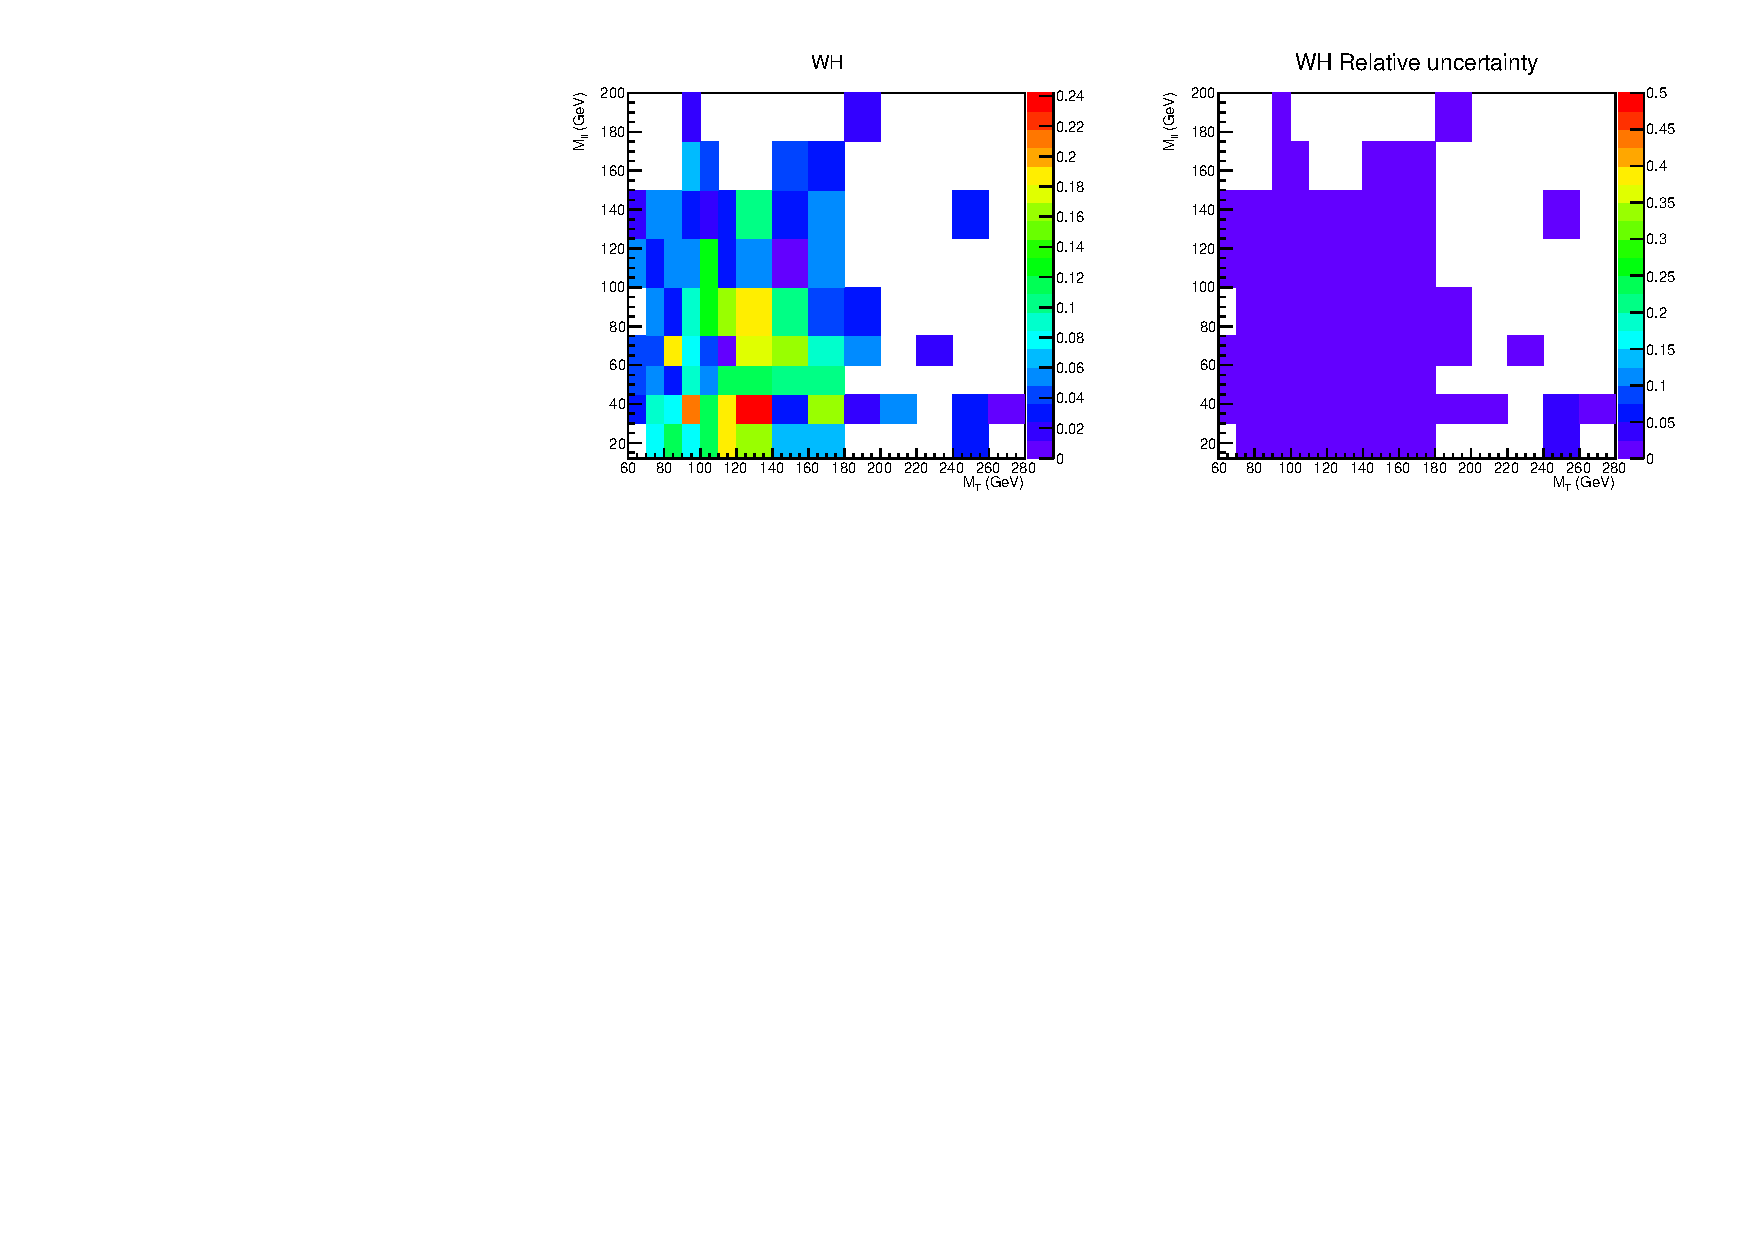
\includegraphics[width=0.8\textwidth]{figures/2dtemplate_WH_mH125_0j.pdf}
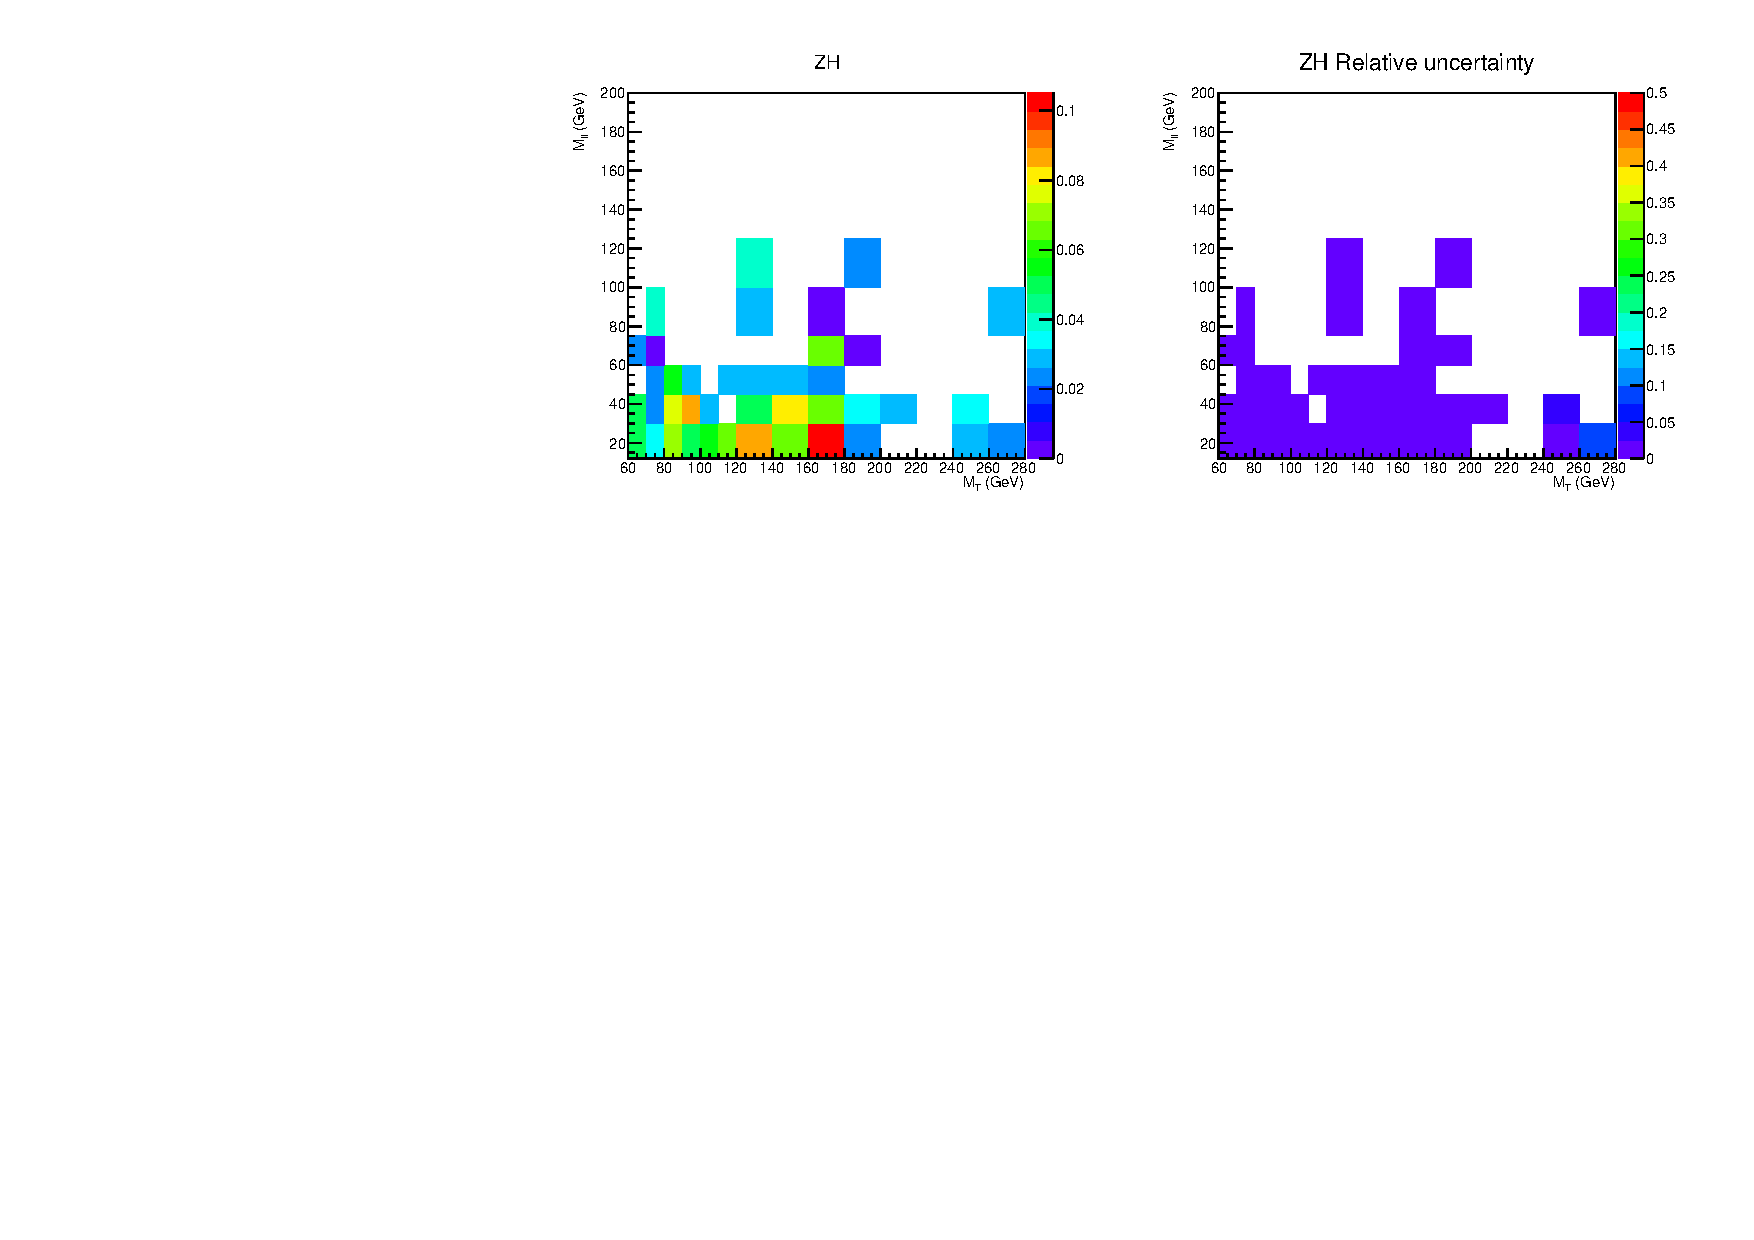
\includegraphics[width=0.8\textwidth]{figures/2dtemplate_ZH_mH125_0j.pdf}
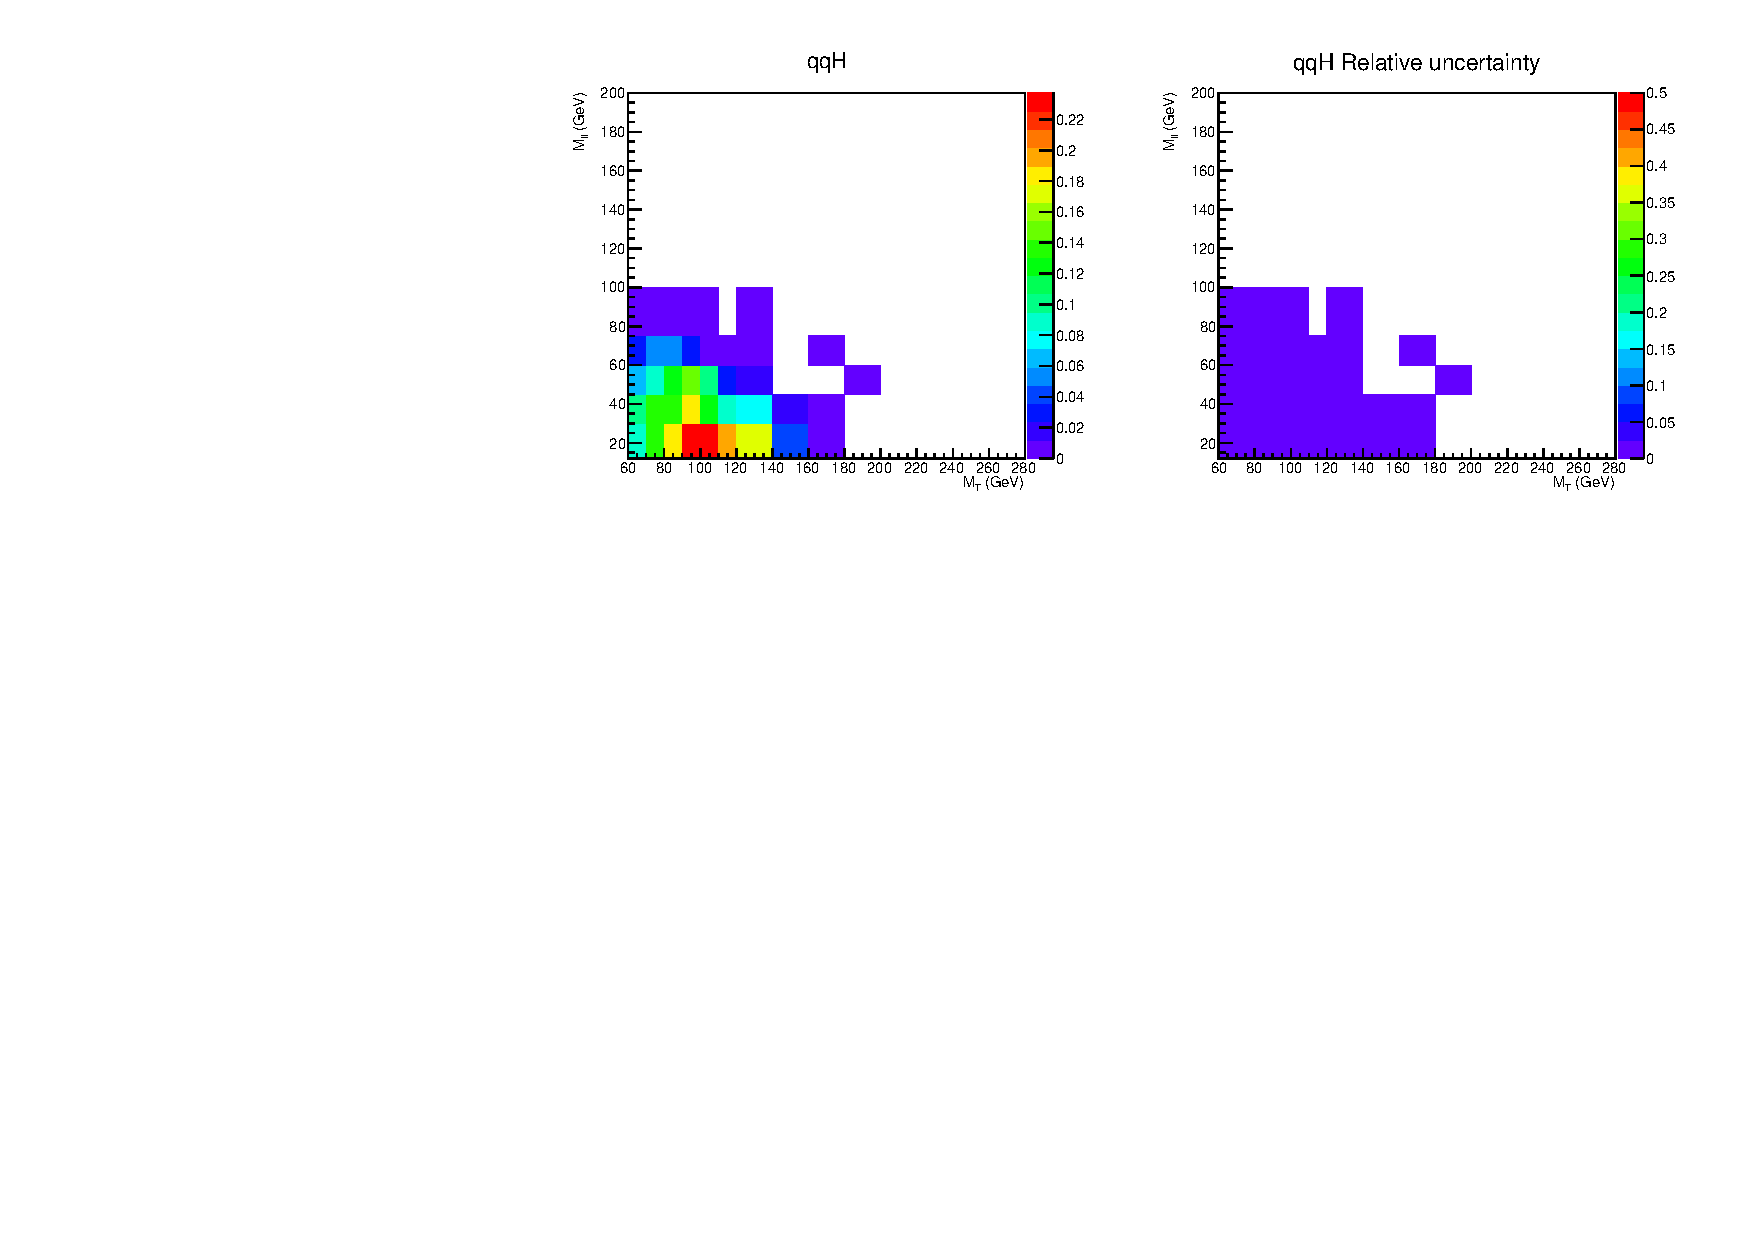
\includegraphics[width=0.8\textwidth]{figures/2dtemplate_qqH_mH125_0j.pdf}
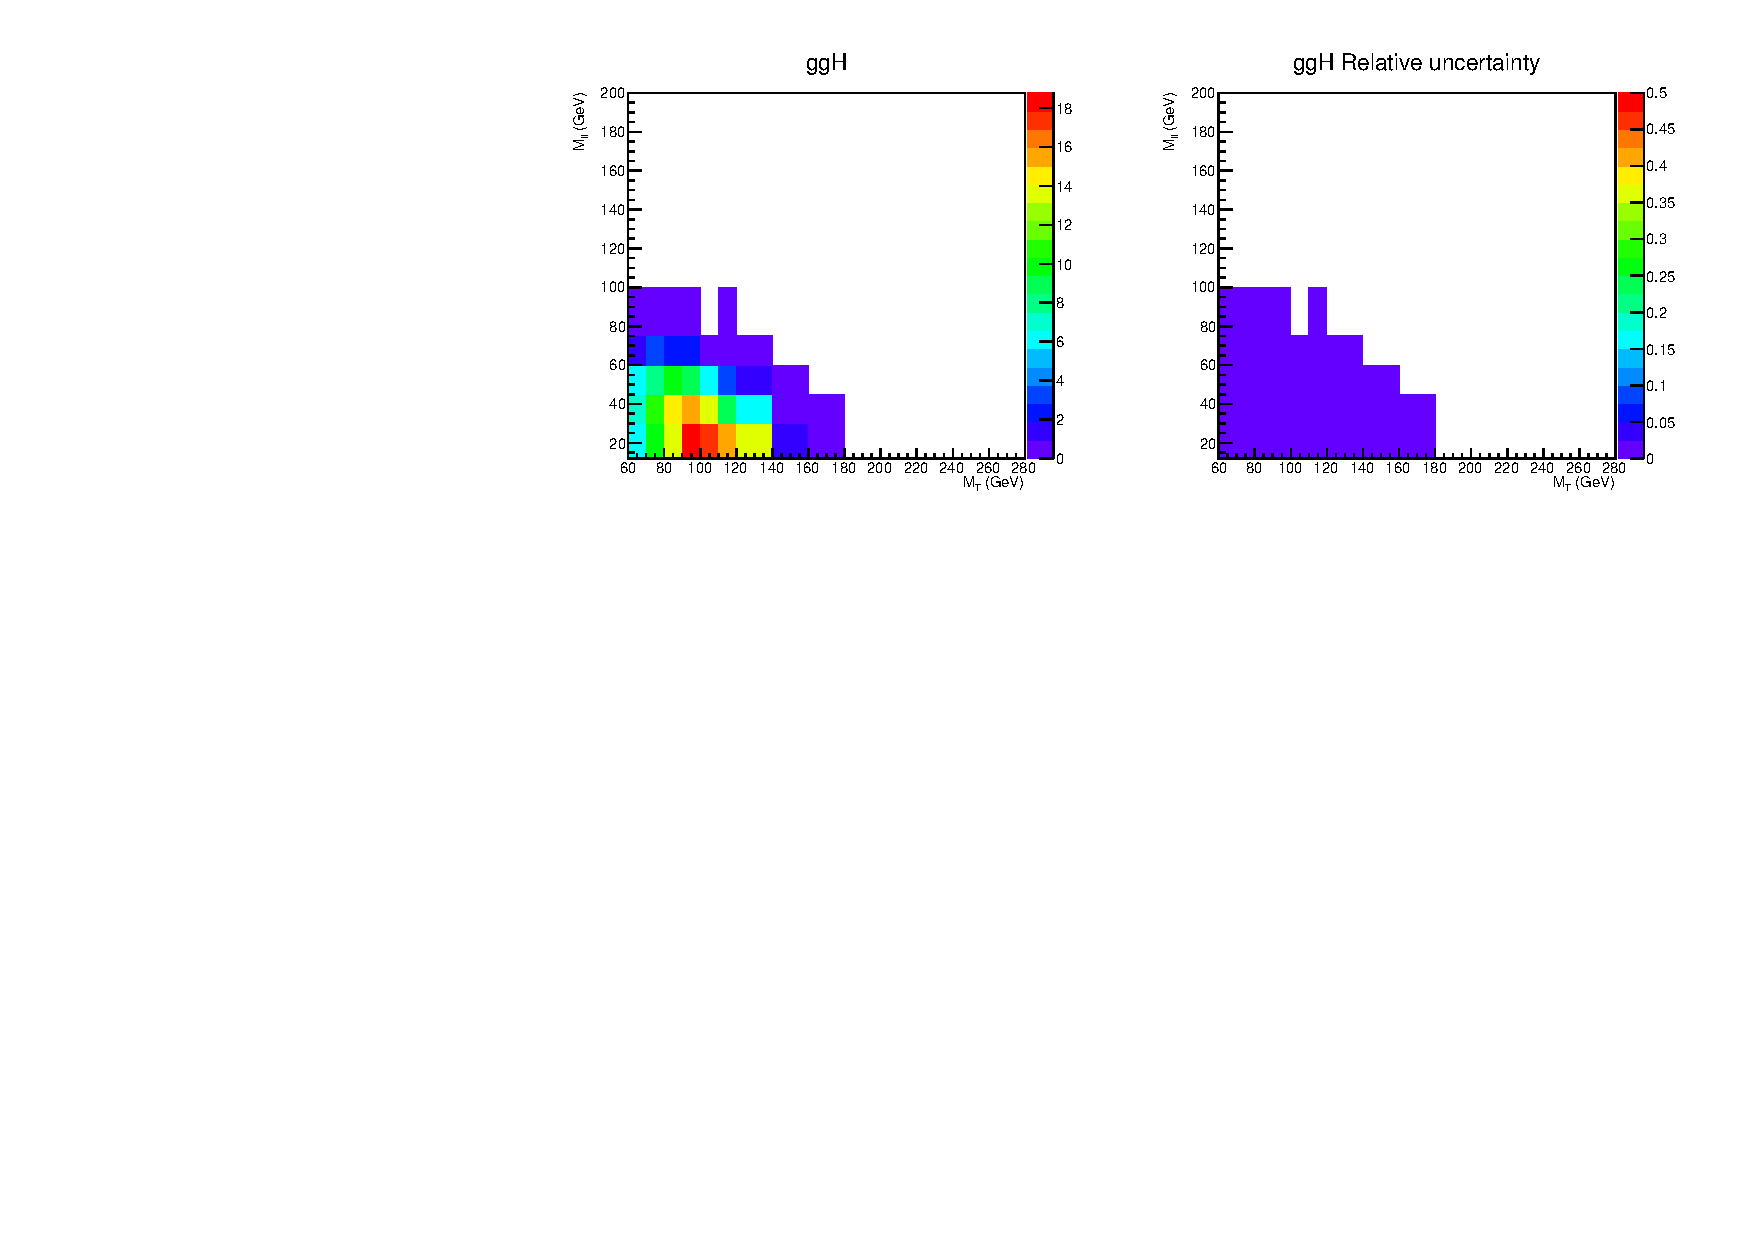
\includegraphics[width=0.8\textwidth]{figures/2dtemplate_ggH_mH125_0j.pdf}
\caption{Templates(left) and relative statistical uncertainty of the MC sample(right) 
of \qqWH, \qqZH, \qqH\ and \ggH. 
The templates are for \mHi\ = 125 \GeV\ analysis in the 0-jet category.}
\label{fig:2dtemplate_125_0j_1}
\end{figure}

\begin{figure}[htp]
\centering
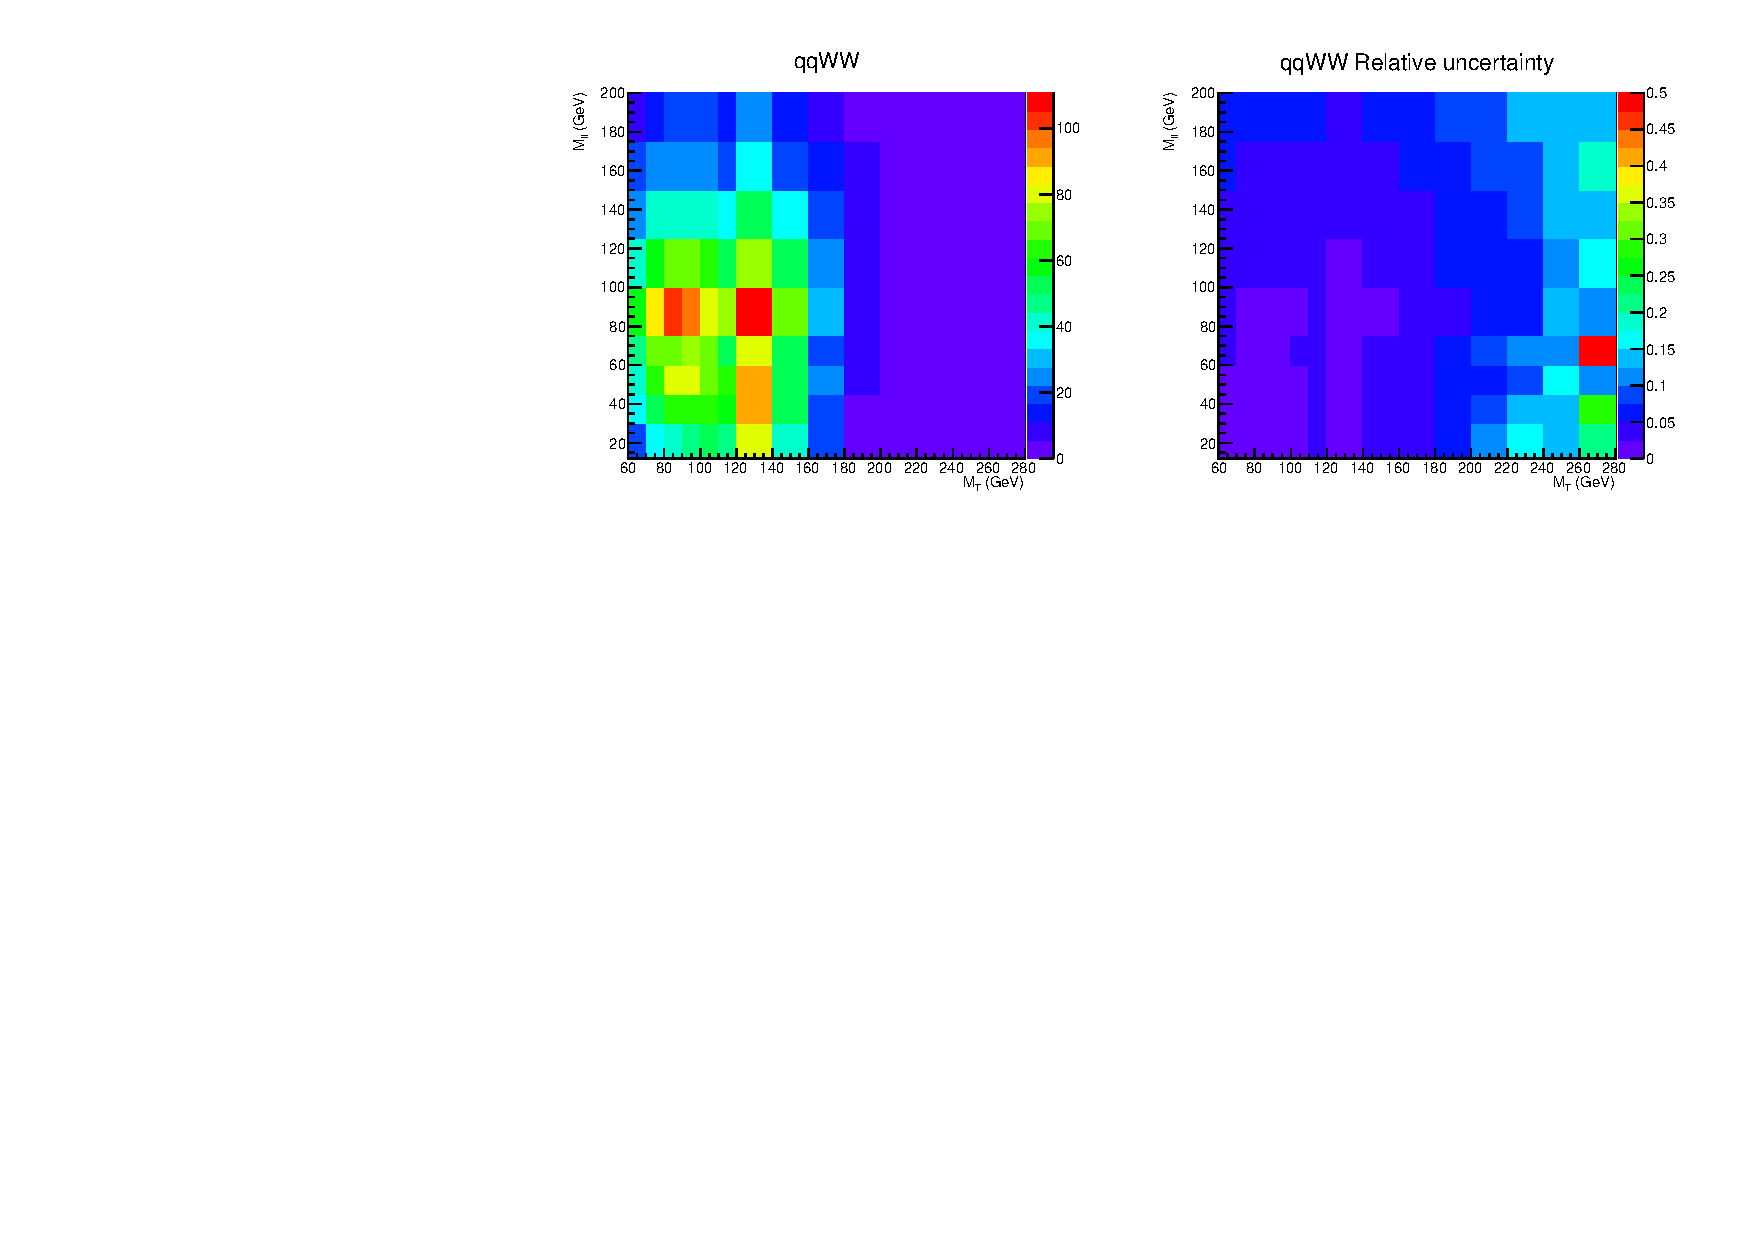
\includegraphics[width=0.8\textwidth]{figures/2dtemplate_qqWW_mH125_0j.pdf}
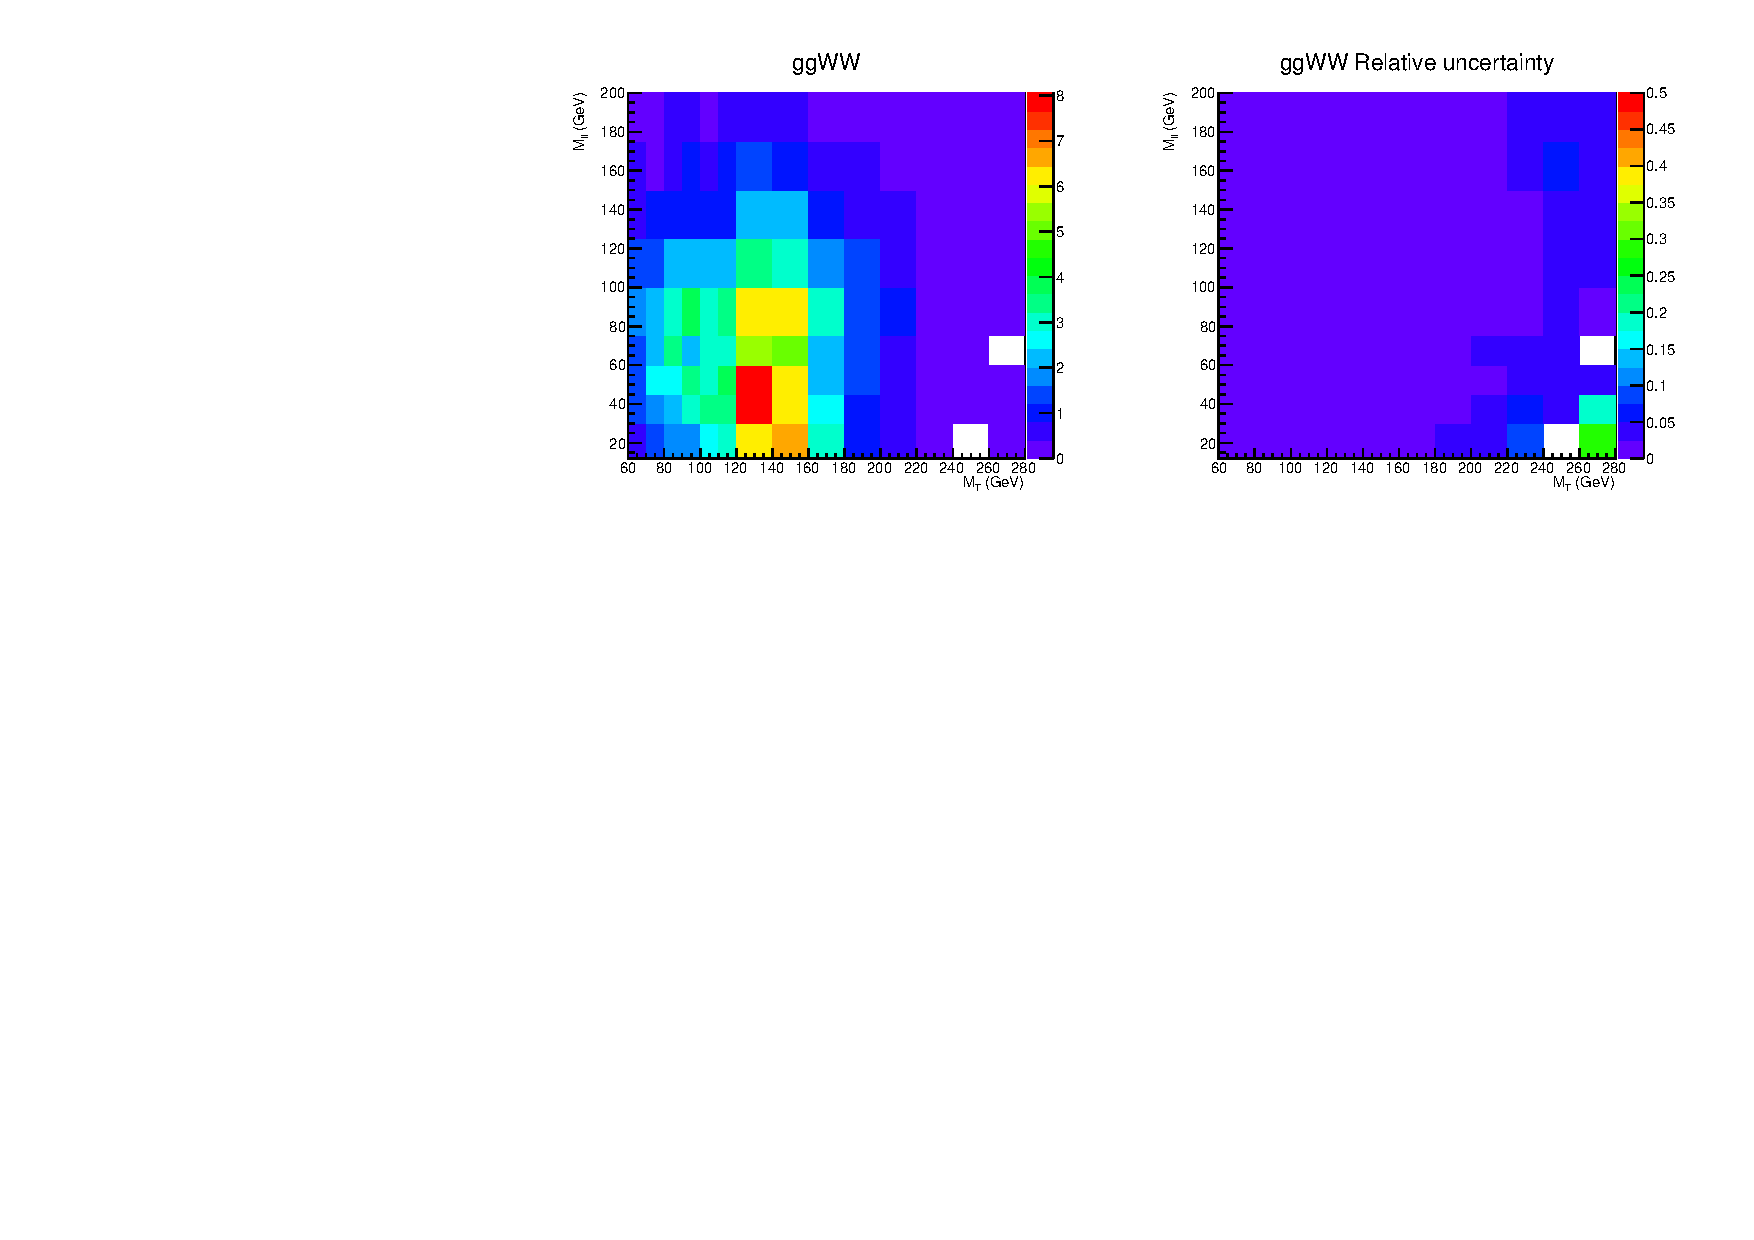
\includegraphics[width=0.8\textwidth]{figures/2dtemplate_ggWW_mH125_0j.pdf}
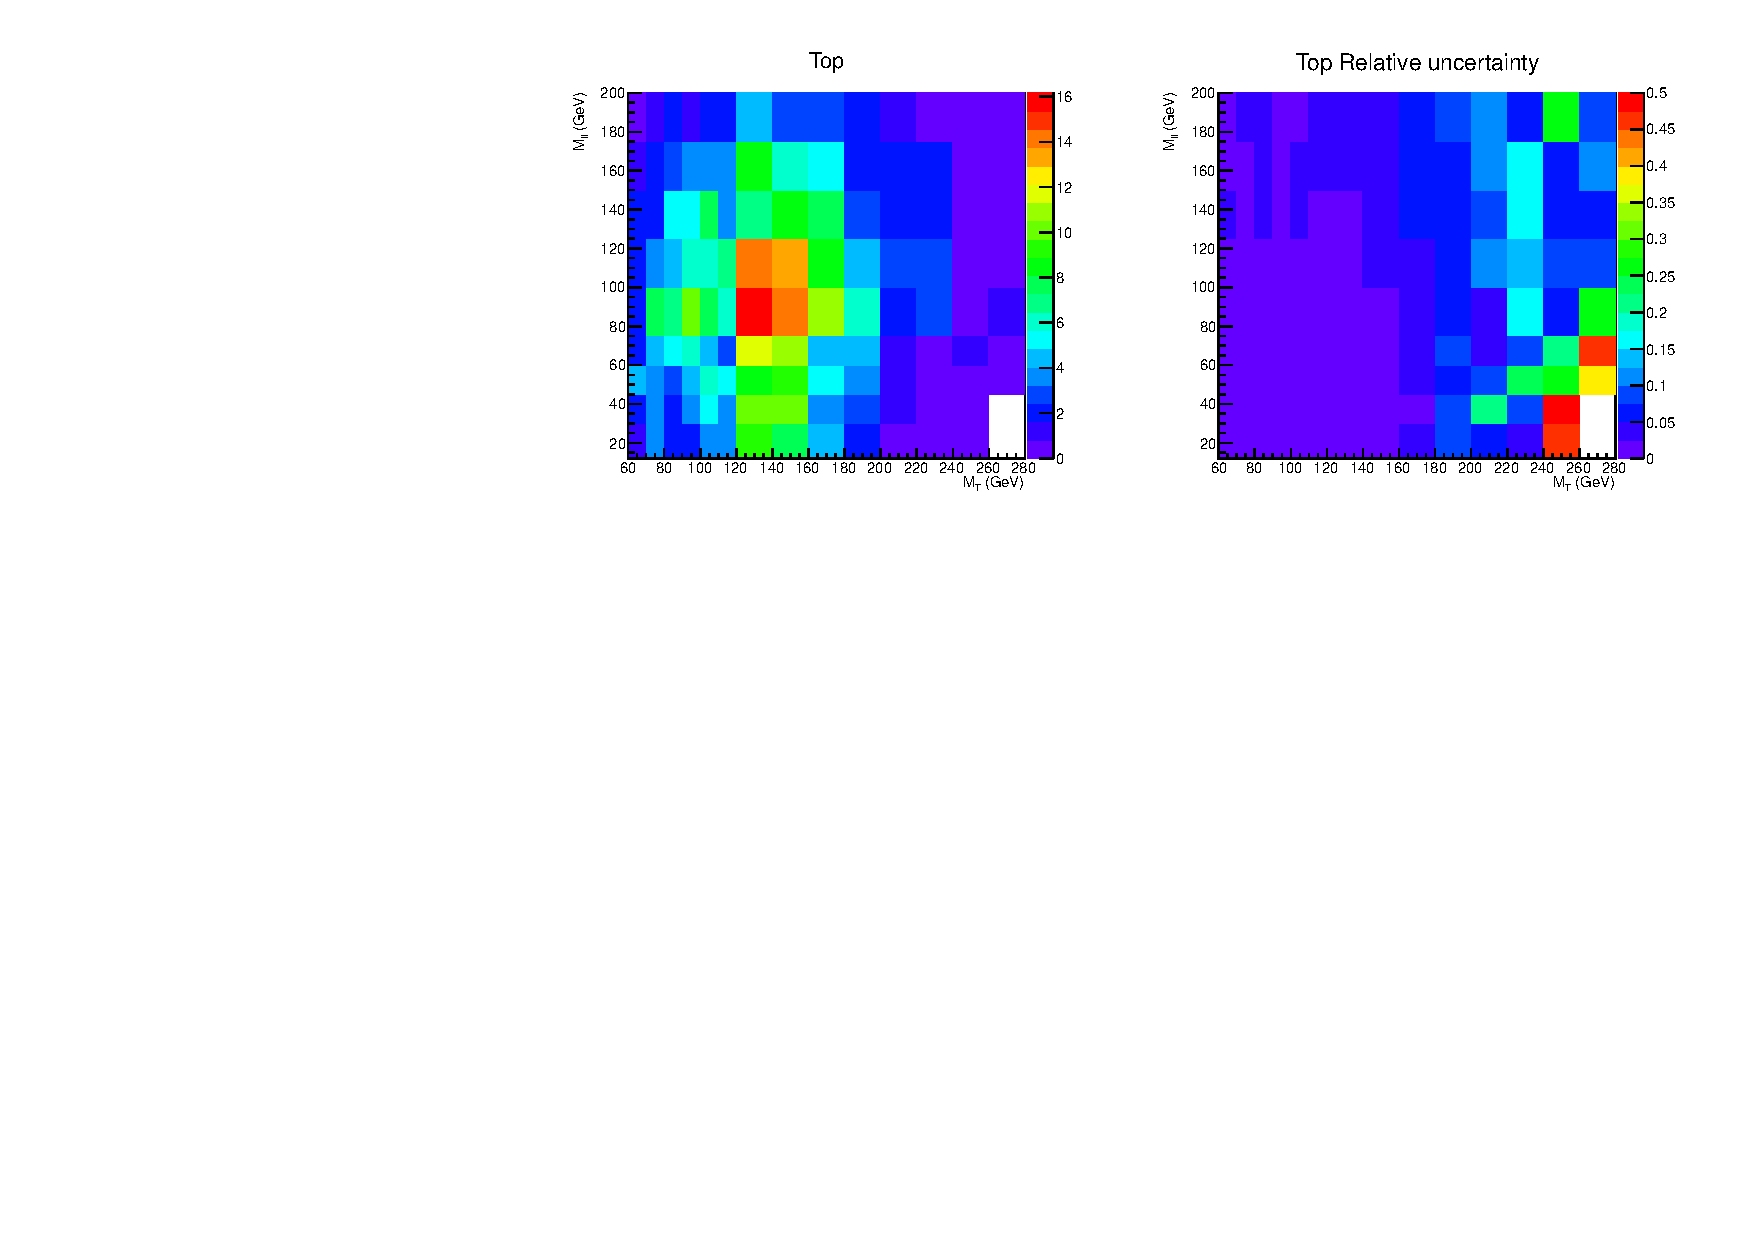
\includegraphics[width=0.8\textwidth]{figures/2dtemplate_Top_mH125_0j.pdf}
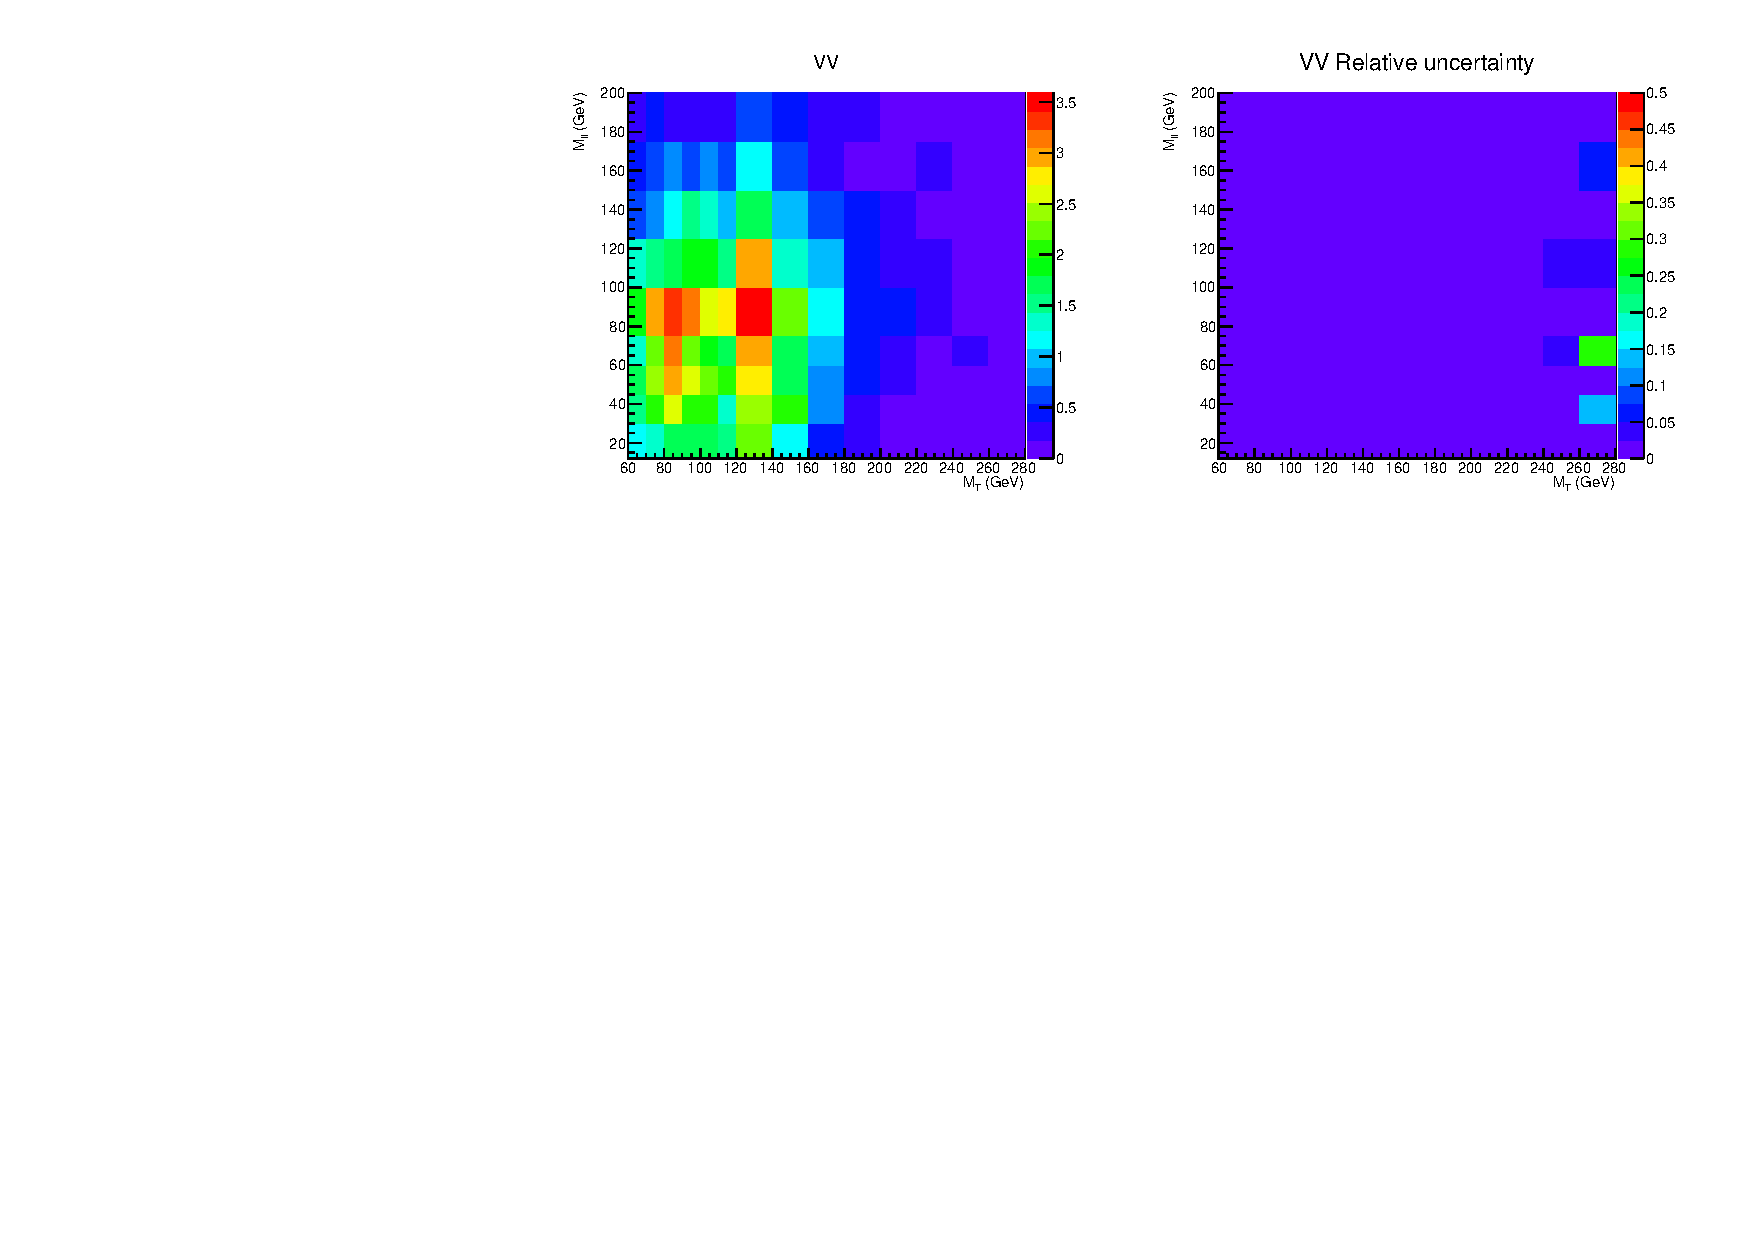
\includegraphics[width=0.8\textwidth]{figures/2dtemplate_VV_mH125_0j.pdf}
\caption{Templates(left) and relative statistical uncertainty of the MC sample(right) 
of \qqww, \ggww, \topbkg\ and \vv. 
The templates are for \mHi\ = 125 \GeV\ analysis in the 0-jet category.}
\label{fig:2dtemplate_125_0j_2}
\end{figure}

\begin{figure}[htp]
\centering
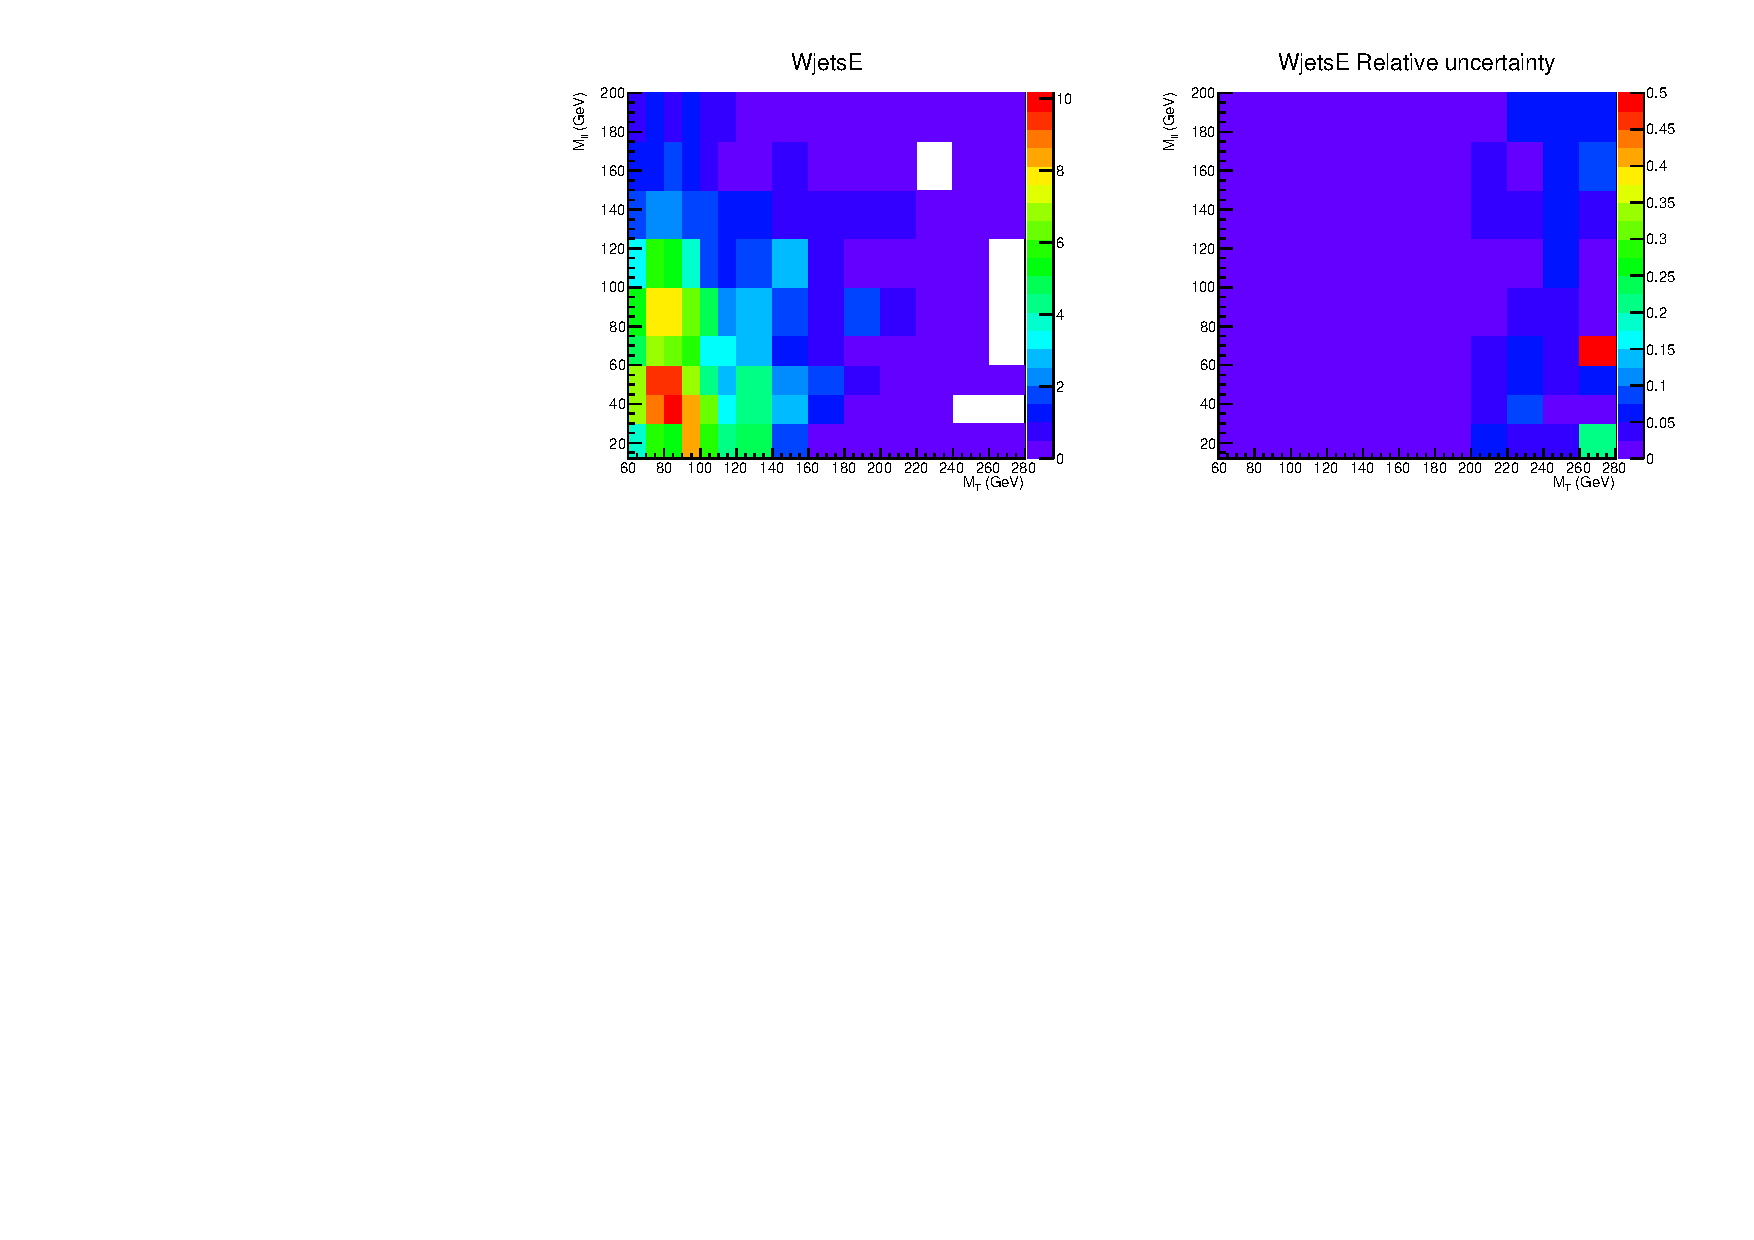
\includegraphics[width=0.8\textwidth]{figures/2dtemplate_WjetsE_mH125_0j.pdf}
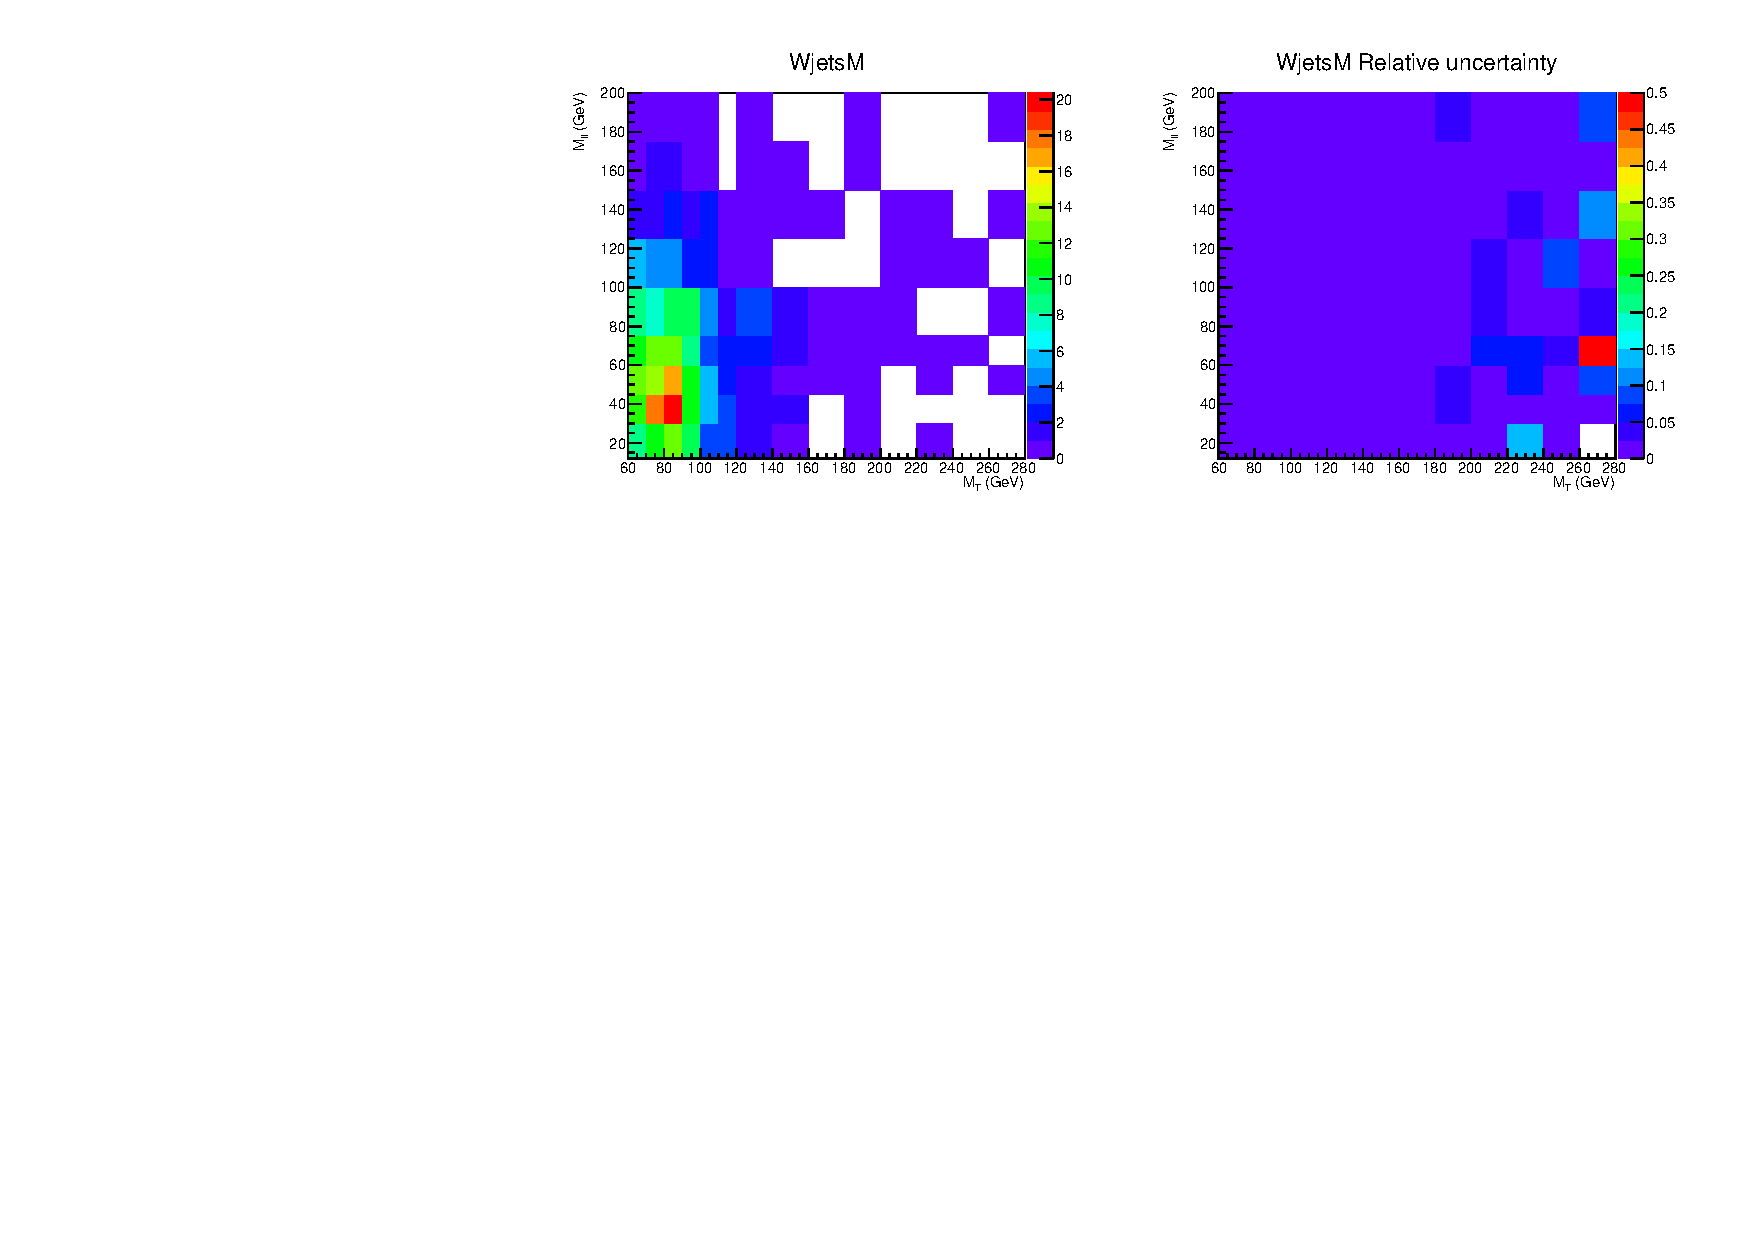
\includegraphics[width=0.8\textwidth]{figures/2dtemplate_WjetsM_mH125_0j.pdf}
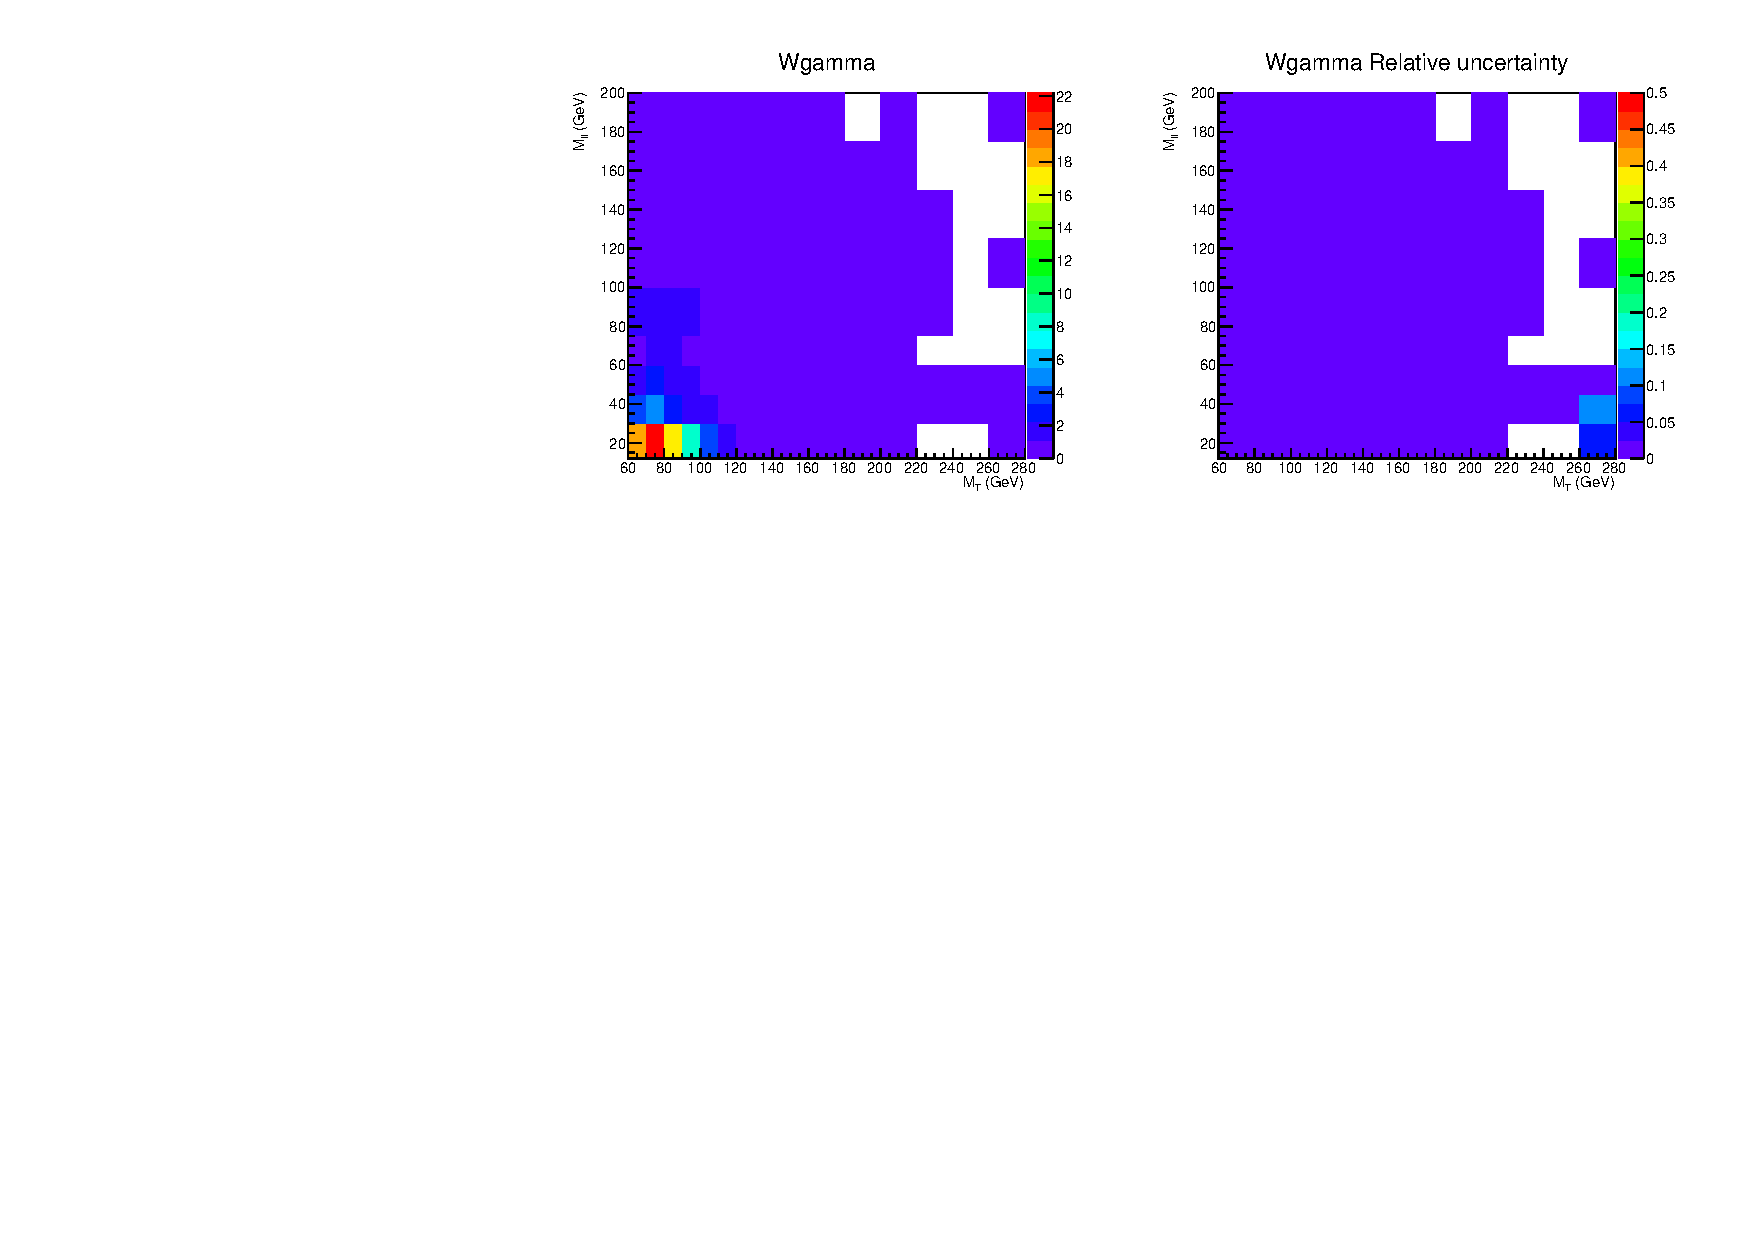
\includegraphics[width=0.8\textwidth]{figures/2dtemplate_Wgamma_mH125_0j.pdf}
\caption{Templates(left) and relative statistical uncertainty of the MC sample(right) 
of \WjetsE, \WjetsM\ and \wgamma. 
The templates are for \mHi\ = 125 \GeV\ analysis in the 0-jet category.}
\label{fig:2dtemplate_125_0j_3}
\end{figure}

\begin{figure}[htp]
\centering
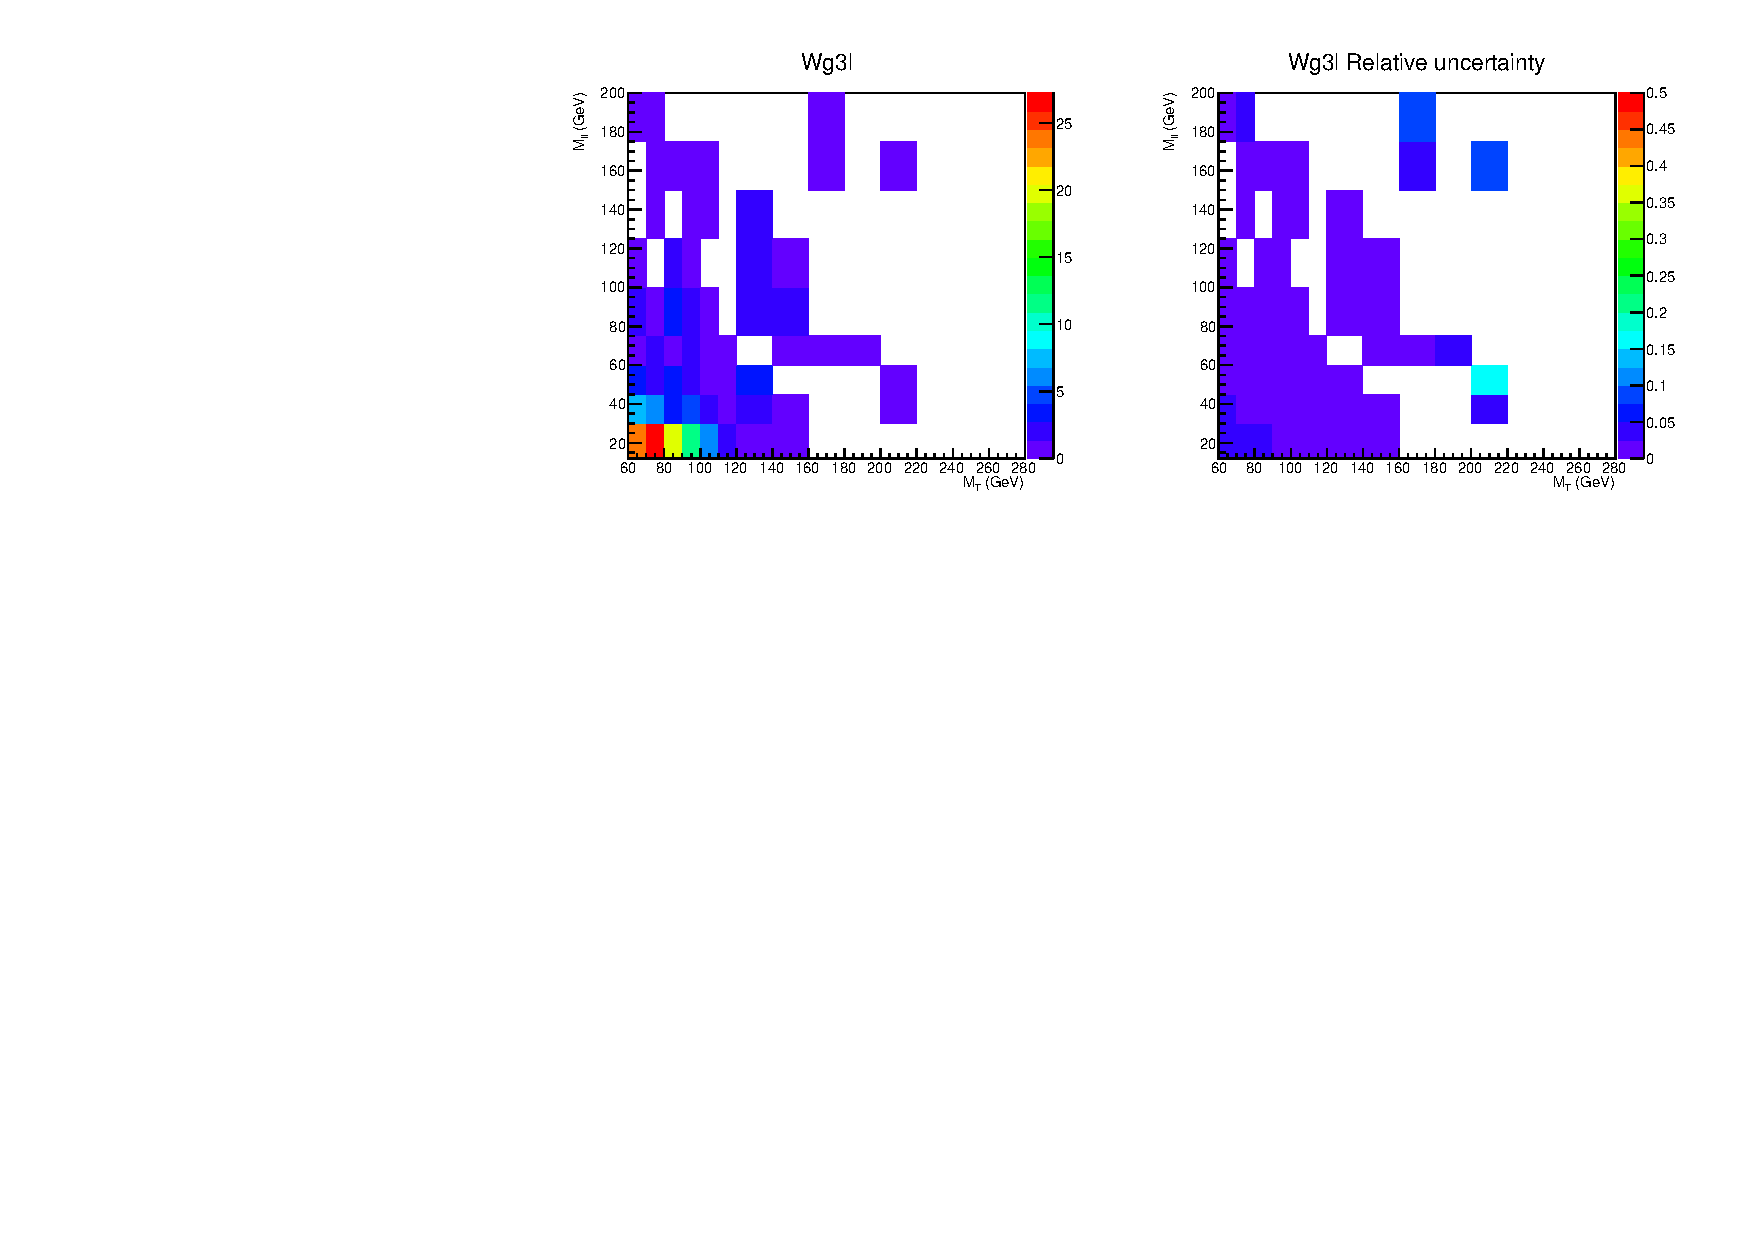
\includegraphics[width=0.8\textwidth]{figures/2dtemplate_Wg3l_mH125_0j.pdf}
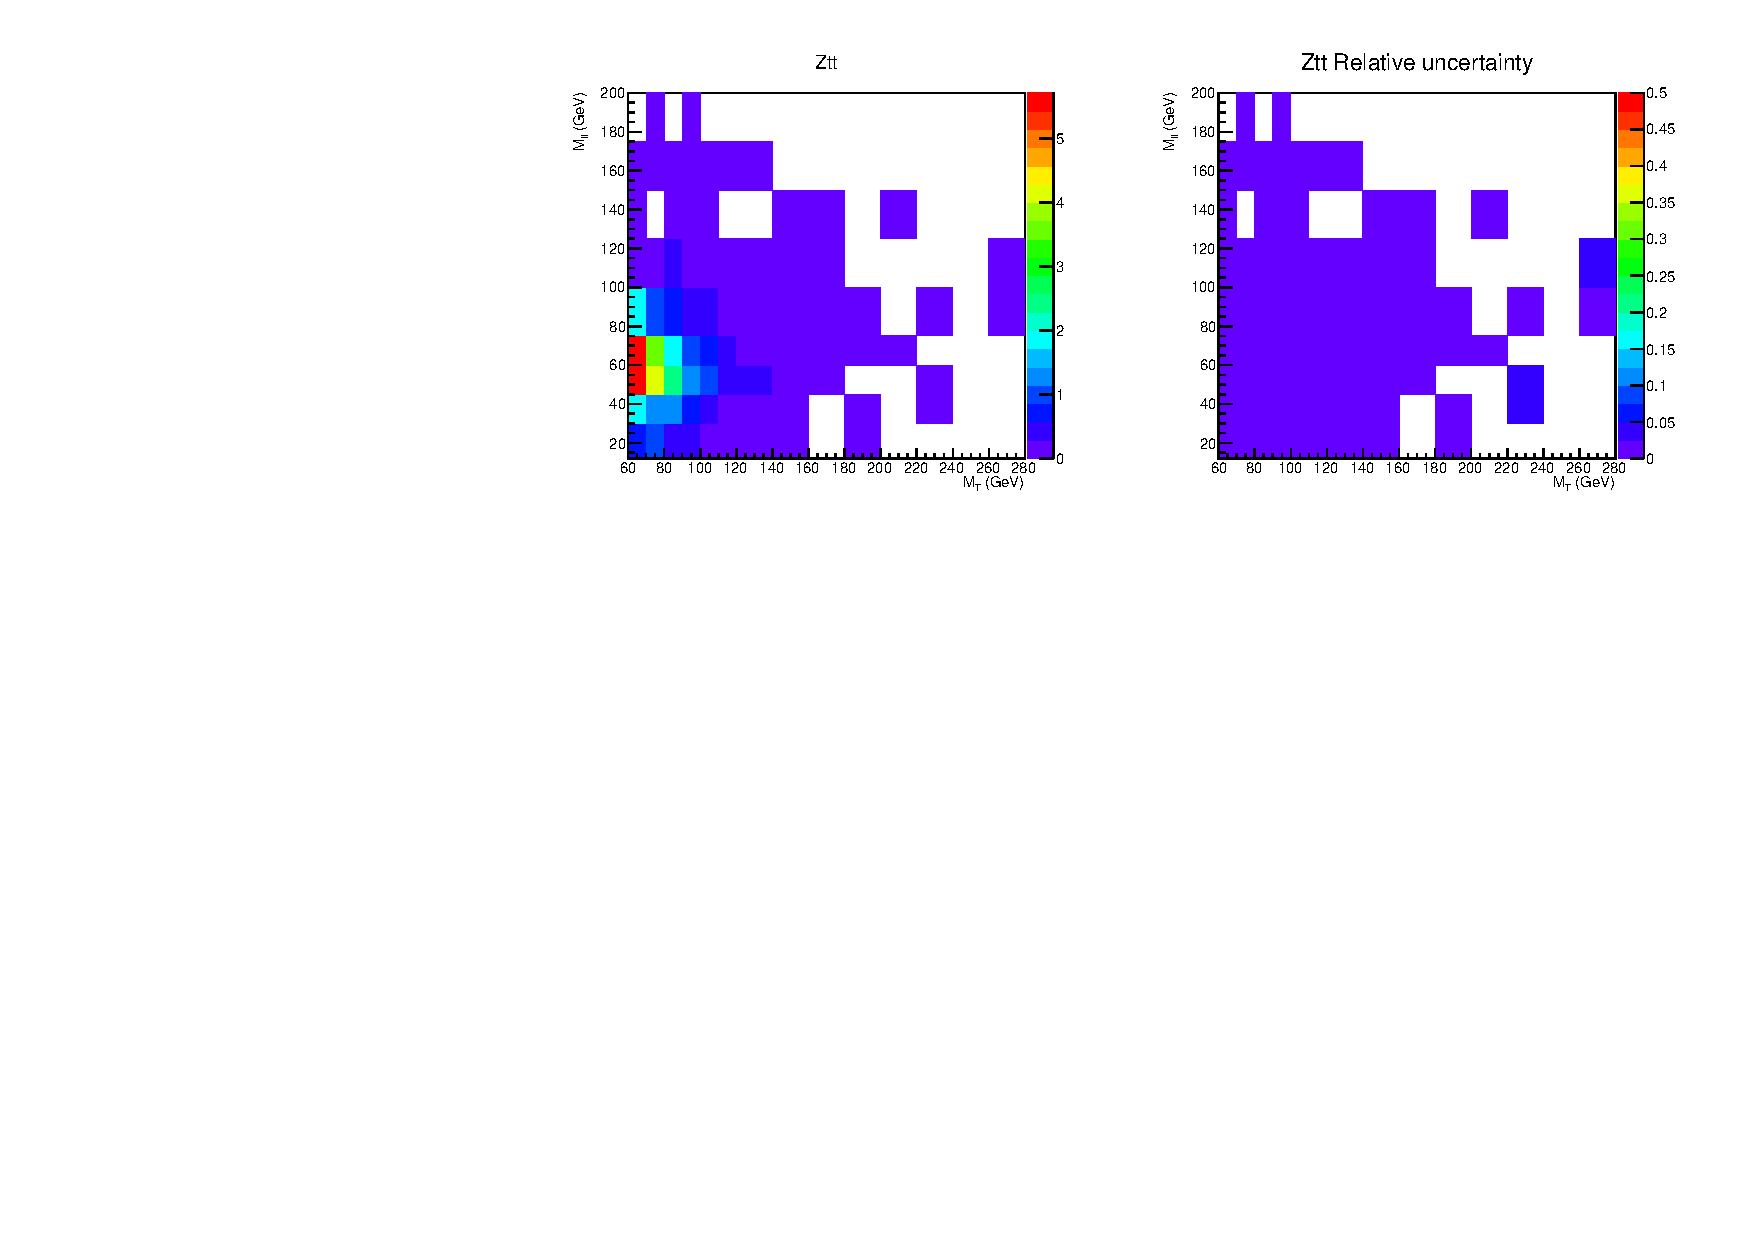
\includegraphics[width=0.8\textwidth]{figures/2dtemplate_Ztt_mH125_0j.pdf}
\caption{Templates(left) and relative statistical uncertainty of the MC sample(right) 
of \wgammastar\ and \ztt. 
The templates are for \mHi\ = 125 \GeV\ analysis in the 0-jet category.}
\label{fig:2dtemplate_125_0j_4}
\end{figure}
